\documentclass{book}
\usepackage[a4paper,top=2.5cm,bottom=2.5cm,left=2.5cm,right=2.5cm]{geometry}
\usepackage{makeidx}
\usepackage{natbib}
\usepackage{graphicx}
\usepackage{multicol}
\usepackage{float}
\usepackage{listings}
\usepackage{color}
\usepackage{ifthen}
\usepackage[table]{xcolor}
\usepackage{textcomp}
\usepackage{alltt}
\usepackage{ifpdf}
\ifpdf
\usepackage[pdftex,
            pagebackref=true,
            colorlinks=true,
            linkcolor=blue,
            unicode
           ]{hyperref}
\else
\usepackage[ps2pdf,
            pagebackref=true,
            colorlinks=true,
            linkcolor=blue,
            unicode
           ]{hyperref}
\usepackage{pspicture}
\fi
\usepackage[utf8]{inputenc}
\usepackage{mathptmx}
\usepackage[scaled=.90]{helvet}
\usepackage{courier}
\usepackage{sectsty}
\usepackage{amssymb}
\usepackage[titles]{tocloft}
\usepackage{doxygen}
\lstset{language=C++,inputencoding=utf8,basicstyle=\footnotesize,breaklines=true,breakatwhitespace=true,tabsize=4,numbers=left }
\makeindex
\setcounter{tocdepth}{3}
\renewcommand{\footrulewidth}{0.4pt}
\renewcommand{\familydefault}{\sfdefault}
\hfuzz=15pt
\setlength{\emergencystretch}{15pt}
\hbadness=750
\tolerance=750
\begin{document}
\hypersetup{pageanchor=false,citecolor=blue}
\begin{titlepage}
\vspace*{7cm}
\begin{center}
{\Large Mage\-Project \\[1ex]\large 2.\-00 }\\
\vspace*{1cm}
{\large Generated by Doxygen 1.8.2}\\
\vspace*{0.5cm}
{\small Mon Sep 17 2012 22:00:24}\\
\end{center}
\end{titlepage}
\clearemptydoublepage
\pagenumbering{roman}
\tableofcontents
\clearemptydoublepage
\pagenumbering{arabic}
\hypersetup{pageanchor=true,citecolor=blue}
\chapter{Hierarchical Index}
\section{Class Hierarchy}
This inheritance list is sorted roughly, but not completely, alphabetically\-:\begin{DoxyCompactList}
\item \contentsline{section}{M\-A\-G\-E\-:\-:Distribution}{\pageref{struct_m_a_g_e_1_1_distribution}}{}
\begin{DoxyCompactList}
\item \contentsline{section}{M\-A\-G\-E\-:\-:M\-S\-Distribution}{\pageref{struct_m_a_g_e_1_1_m_s_distribution}}{}
\end{DoxyCompactList}
\item \contentsline{section}{M\-A\-G\-E\-:\-:Engine}{\pageref{class_m_a_g_e_1_1_engine}}{}
\item \contentsline{section}{M\-A\-G\-E\-:\-:Frame}{\pageref{struct_m_a_g_e_1_1_frame}}{}
\item \contentsline{section}{M\-A\-G\-E\-:\-:Label}{\pageref{class_m_a_g_e_1_1_label}}{}
\item \contentsline{section}{M\-A\-G\-E\-:\-:Label\-Memory}{\pageref{class_m_a_g_e_1_1_label_memory}}{}
\item \contentsline{section}{M\-A\-G\-E\-:\-:Label\-Queue}{\pageref{class_m_a_g_e_1_1_label_queue}}{}
\item \contentsline{section}{M\-A\-G\-E\-:\-:Mage}{\pageref{class_m_a_g_e_1_1_mage}}{}
\item \contentsline{section}{M\-A\-G\-E\-:\-:Mem\-Queue$<$ Item $>$}{\pageref{class_m_a_g_e_1_1_mem_queue}}{}
\item \contentsline{section}{M\-A\-G\-E\-:\-:Mem\-Queue$<$ Frame $>$}{\pageref{class_m_a_g_e_1_1_mem_queue}}{}
\begin{DoxyCompactList}
\item \contentsline{section}{M\-A\-G\-E\-:\-:Frame\-Queue}{\pageref{class_m_a_g_e_1_1_frame_queue}}{}
\end{DoxyCompactList}
\item \contentsline{section}{M\-A\-G\-E\-:\-:Mem\-Queue$<$ Model $>$}{\pageref{class_m_a_g_e_1_1_mem_queue}}{}
\begin{DoxyCompactList}
\item \contentsline{section}{M\-A\-G\-E\-:\-:Model\-Queue}{\pageref{class_m_a_g_e_1_1_model_queue}}{}
\end{DoxyCompactList}
\item \contentsline{section}{M\-A\-G\-E\-:\-:Model}{\pageref{class_m_a_g_e_1_1_model}}{}
\item \contentsline{section}{M\-A\-G\-E\-:\-:Model\-Memory}{\pageref{class_m_a_g_e_1_1_model_memory}}{}
\item \contentsline{section}{M\-A\-G\-E\-:\-:Model\-Queue\-Memory}{\pageref{class_m_a_g_e_1_1_model_queue_memory}}{}
\item \contentsline{section}{M\-A\-G\-E\-:\-:State}{\pageref{struct_m_a_g_e_1_1_state}}{}
\item \contentsline{section}{M\-A\-G\-E\-:\-:Vocoder}{\pageref{class_m_a_g_e_1_1_vocoder}}{}
\end{DoxyCompactList}

\chapter{Class Index}
\section{Class List}
Here are the classes, structs, unions and interfaces with brief descriptions\-:\begin{DoxyCompactList}
\item\contentsline{section}{\hyperlink{struct_m_a_g_e_1_1_distribution}{M\-A\-G\-E\-::\-Distribution} \\*Definition of a gaussian distribution }{\pageref{struct_m_a_g_e_1_1_distribution}}{}
\item\contentsline{section}{\hyperlink{class_m_a_g_e_1_1_engine}{M\-A\-G\-E\-::\-Engine} }{\pageref{class_m_a_g_e_1_1_engine}}{}
\item\contentsline{section}{\hyperlink{struct_m_a_g_e_1_1_frame}{M\-A\-G\-E\-::\-Frame} }{\pageref{struct_m_a_g_e_1_1_frame}}{}
\item\contentsline{section}{\hyperlink{class_m_a_g_e_1_1_frame_queue}{M\-A\-G\-E\-::\-Frame\-Queue} }{\pageref{class_m_a_g_e_1_1_frame_queue}}{}
\item\contentsline{section}{\hyperlink{class_m_a_g_e_1_1_label}{M\-A\-G\-E\-::\-Label} }{\pageref{class_m_a_g_e_1_1_label}}{}
\item\contentsline{section}{\hyperlink{class_m_a_g_e_1_1_label_memory}{M\-A\-G\-E\-::\-Label\-Memory} }{\pageref{class_m_a_g_e_1_1_label_memory}}{}
\item\contentsline{section}{\hyperlink{class_m_a_g_e_1_1_label_queue}{M\-A\-G\-E\-::\-Label\-Queue} }{\pageref{class_m_a_g_e_1_1_label_queue}}{}
\item\contentsline{section}{\hyperlink{class_m_a_g_e_1_1_mage}{M\-A\-G\-E\-::\-Mage} }{\pageref{class_m_a_g_e_1_1_mage}}{}
\item\contentsline{section}{\hyperlink{class_m_a_g_e_1_1_mem_queue}{M\-A\-G\-E\-::\-Mem\-Queue$<$ Item $>$} }{\pageref{class_m_a_g_e_1_1_mem_queue}}{}
\item\contentsline{section}{\hyperlink{class_m_a_g_e_1_1_model}{M\-A\-G\-E\-::\-Model} }{\pageref{class_m_a_g_e_1_1_model}}{}
\item\contentsline{section}{\hyperlink{class_m_a_g_e_1_1_model_memory}{M\-A\-G\-E\-::\-Model\-Memory} \\*The memory used for every model }{\pageref{class_m_a_g_e_1_1_model_memory}}{}
\item\contentsline{section}{\hyperlink{class_m_a_g_e_1_1_model_queue}{M\-A\-G\-E\-::\-Model\-Queue} }{\pageref{class_m_a_g_e_1_1_model_queue}}{}
\item\contentsline{section}{\hyperlink{class_m_a_g_e_1_1_model_queue_memory}{M\-A\-G\-E\-::\-Model\-Queue\-Memory} }{\pageref{class_m_a_g_e_1_1_model_queue_memory}}{}
\item\contentsline{section}{\hyperlink{struct_m_a_g_e_1_1_m_s_distribution}{M\-A\-G\-E\-::\-M\-S\-Distribution} \\*Definition of an N\-S\-D gaussian distribution }{\pageref{struct_m_a_g_e_1_1_m_s_distribution}}{}
\item\contentsline{section}{\hyperlink{struct_m_a_g_e_1_1_state}{M\-A\-G\-E\-::\-State} \\*Definition of the H\-M\-Ms }{\pageref{struct_m_a_g_e_1_1_state}}{}
\item\contentsline{section}{\hyperlink{class_m_a_g_e_1_1_vocoder}{M\-A\-G\-E\-::\-Vocoder} }{\pageref{class_m_a_g_e_1_1_vocoder}}{}
\end{DoxyCompactList}

\chapter{File Index}
\section{File List}
Here is a list of all documented files with brief descriptions\-:\begin{DoxyCompactList}
\item\contentsline{section}{/\-Users/\-Maipn/\-Documents/my\-Libs/\-M\-A\-G\-E/magelib-\/2.\-00/src/\hyperlink{_constants_8h}{Constants.\-h} }{\pageref{_constants_8h}}{}
\item\contentsline{section}{/\-Users/\-Maipn/\-Documents/my\-Libs/\-M\-A\-G\-E/magelib-\/2.\-00/src/{\bfseries Distribution.\-h} }{\pageref{_distribution_8h}}{}
\item\contentsline{section}{/\-Users/\-Maipn/\-Documents/my\-Libs/\-M\-A\-G\-E/magelib-\/2.\-00/src/\hyperlink{_frame_8h}{Frame.\-h} \\*Synthesis frame class }{\pageref{_frame_8h}}{}
\item\contentsline{section}{/\-Users/\-Maipn/\-Documents/my\-Libs/\-M\-A\-G\-E/magelib-\/2.\-00/src/\hyperlink{_frame_queue_8cpp}{Frame\-Queue.\-cpp} \\*Frame ringbuffer\-: used to exchange speech parameters with the synthesis thread }{\pageref{_frame_queue_8cpp}}{}
\item\contentsline{section}{/\-Users/\-Maipn/\-Documents/my\-Libs/\-M\-A\-G\-E/magelib-\/2.\-00/src/\hyperlink{_frame_queue_8h}{Frame\-Queue.\-h} \\*Frame ringbuffer\-: used to exchange speech parameters with the synthesis thread }{\pageref{_frame_queue_8h}}{}
\item\contentsline{section}{/\-Users/\-Maipn/\-Documents/my\-Libs/\-M\-A\-G\-E/magelib-\/2.\-00/src/\hyperlink{hts_8cpp}{hts.\-cpp} }{\pageref{hts_8cpp}}{}
\item\contentsline{section}{/\-Users/\-Maipn/\-Documents/my\-Libs/\-M\-A\-G\-E/magelib-\/2.\-00/src/\hyperlink{hts_8h}{hts.\-h} }{\pageref{hts_8h}}{}
\item\contentsline{section}{/\-Users/\-Maipn/\-Documents/my\-Libs/\-M\-A\-G\-E/magelib-\/2.\-00/src/\hyperlink{_label_8cpp}{Label.\-cpp} \\*Label class\-: store the label string + time tags and either duration is forced }{\pageref{_label_8cpp}}{}
\item\contentsline{section}{/\-Users/\-Maipn/\-Documents/my\-Libs/\-M\-A\-G\-E/magelib-\/2.\-00/src/\hyperlink{_label_8h}{Label.\-h} \\*Label class\-: store the label string + time tags and either duration is forced }{\pageref{_label_8h}}{}
\item\contentsline{section}{/\-Users/\-Maipn/\-Documents/my\-Libs/\-M\-A\-G\-E/magelib-\/2.\-00/src/\hyperlink{_label_queue_8cpp}{Label\-Queue.\-cpp} \\*Label queue class\-: used to exchange the labels between the different threads; we could not inherint from Mem\-Queue because Label is not a P\-O\-D type -\/$>$ memory issues }{\pageref{_label_queue_8cpp}}{}
\item\contentsline{section}{/\-Users/\-Maipn/\-Documents/my\-Libs/\-M\-A\-G\-E/magelib-\/2.\-00/src/\hyperlink{_label_queue_8h}{Label\-Queue.\-h} \\*Label queue class\-: used to exchange the labels between the different threads; we could not inherint from Mem\-Queue because Label is not a P\-O\-D type -\/$>$ memory issues }{\pageref{_label_queue_8h}}{}
\item\contentsline{section}{/\-Users/\-Maipn/\-Documents/my\-Libs/\-M\-A\-G\-E/magelib-\/2.\-00/src/\hyperlink{mage_8cpp}{mage.\-cpp} }{\pageref{mage_8cpp}}{}
\item\contentsline{section}{/\-Users/\-Maipn/\-Documents/my\-Libs/\-M\-A\-G\-E/magelib-\/2.\-00/src/\hyperlink{mage_8h}{mage.\-h} }{\pageref{mage_8h}}{}
\item\contentsline{section}{/\-Users/\-Maipn/\-Documents/my\-Libs/\-M\-A\-G\-E/magelib-\/2.\-00/src/\hyperlink{_math_functions_8cpp}{Math\-Functions.\-cpp} }{\pageref{_math_functions_8cpp}}{}
\item\contentsline{section}{/\-Users/\-Maipn/\-Documents/my\-Libs/\-M\-A\-G\-E/magelib-\/2.\-00/src/\hyperlink{_math_functions_8h}{Math\-Functions.\-h} }{\pageref{_math_functions_8h}}{}
\item\contentsline{section}{/\-Users/\-Maipn/\-Documents/my\-Libs/\-M\-A\-G\-E/magelib-\/2.\-00/src/\hyperlink{_mem_queue_8h}{Mem\-Queue.\-h} \\*Memory-\/efficient lock-\/free ringbuffer\-: push and template P\-O\-D data with memcpy() and inform on the state of the buffer }{\pageref{_mem_queue_8h}}{}
\item\contentsline{section}{/\-Users/\-Maipn/\-Documents/my\-Libs/\-M\-A\-G\-E/magelib-\/2.\-00/src/\hyperlink{_model_8cpp}{Model.\-cpp} }{\pageref{_model_8cpp}}{}
\item\contentsline{section}{/\-Users/\-Maipn/\-Documents/my\-Libs/\-M\-A\-G\-E/magelib-\/2.\-00/src/\hyperlink{_model_8h}{Model.\-h} \\*H\-M\-M class\-: a bunch of states }{\pageref{_model_8h}}{}
\item\contentsline{section}{/\-Users/\-Maipn/\-Documents/my\-Libs/\-M\-A\-G\-E/magelib-\/2.\-00/src/\hyperlink{_model_queue_8cpp}{Model\-Queue.\-cpp} \\*Model ringbuffer\-: used to store statistical models + special generate()function that takes a lookup window and generates oldest-\/label frames }{\pageref{_model_queue_8cpp}}{}
\item\contentsline{section}{/\-Users/\-Maipn/\-Documents/my\-Libs/\-M\-A\-G\-E/magelib-\/2.\-00/src/\hyperlink{_model_queue_8h}{Model\-Queue.\-h} \\*Model ringbuffer\-: used to store statistical models + special generate()function that takes a lookup window and generates oldest-\/label frames }{\pageref{_model_queue_8h}}{}
\item\contentsline{section}{/\-Users/\-Maipn/\-Documents/my\-Libs/\-M\-A\-G\-E/magelib-\/2.\-00/src/{\bfseries M\-S\-Distribution.\-h} }{\pageref{_m_s_distribution_8h}}{}
\item\contentsline{section}{/\-Users/\-Maipn/\-Documents/my\-Libs/\-M\-A\-G\-E/magelib-\/2.\-00/src/{\bfseries State.\-h} }{\pageref{_state_8h}}{}
\item\contentsline{section}{/\-Users/\-Maipn/\-Documents/my\-Libs/\-M\-A\-G\-E/magelib-\/2.\-00/src/\hyperlink{_vocoder_8cpp}{Vocoder.\-cpp} }{\pageref{_vocoder_8cpp}}{}
\item\contentsline{section}{/\-Users/\-Maipn/\-Documents/my\-Libs/\-M\-A\-G\-E/magelib-\/2.\-00/src/\hyperlink{_vocoder_8h}{Vocoder.\-h} }{\pageref{_vocoder_8h}}{}
\end{DoxyCompactList}

\chapter{Class Documentation}
\hypertarget{struct_m_a_g_e_1_1_distribution}{\section{M\-A\-G\-E\-:\-:Distribution Struct Reference}
\label{struct_m_a_g_e_1_1_distribution}\index{M\-A\-G\-E\-::\-Distribution@{M\-A\-G\-E\-::\-Distribution}}
}


Definition of a gaussian distribution.  




{\ttfamily \#include $<$Distribution.\-h$>$}

Inheritance diagram for M\-A\-G\-E\-:\-:Distribution\-:\begin{figure}[H]
\begin{center}
\leavevmode
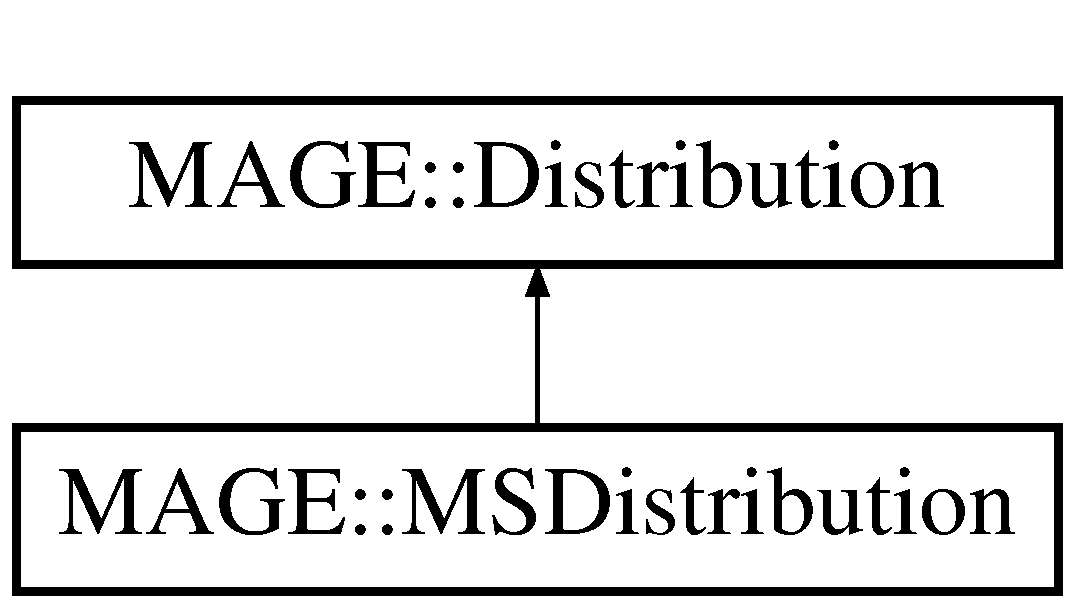
\includegraphics[height=2.000000cm]{struct_m_a_g_e_1_1_distribution}
\end{center}
\end{figure}
\subsection*{Public Attributes}
\begin{DoxyCompactItemize}
\item 
\hypertarget{struct_m_a_g_e_1_1_distribution_a604ebb36706e149529946d2028a178eb}{double \hyperlink{struct_m_a_g_e_1_1_distribution_a604ebb36706e149529946d2028a178eb}{mean}}\label{struct_m_a_g_e_1_1_distribution_a604ebb36706e149529946d2028a178eb}

\begin{DoxyCompactList}\small\item\em It contains the mean value of a gaussian distribution. \end{DoxyCompactList}\item 
\hypertarget{struct_m_a_g_e_1_1_distribution_a9e2f2aa03bb780e60bb402d6eb5c941d}{double \hyperlink{struct_m_a_g_e_1_1_distribution_a9e2f2aa03bb780e60bb402d6eb5c941d}{vari}}\label{struct_m_a_g_e_1_1_distribution_a9e2f2aa03bb780e60bb402d6eb5c941d}

\begin{DoxyCompactList}\small\item\em It contains the variance value of a gaussian distribution. \end{DoxyCompactList}\end{DoxyCompactItemize}


\subsection{Detailed Description}
Definition of a gaussian distribution. 

This struct is used to define a gaussian distribution given the mean and variance as parameters.

\begin{DoxyAuthor}{Authors}
Maria Astrinaki, Alexis Moinet, Geoffrey Wilfart, Nicolas d'Alessandro, Thierry Dutoit
\end{DoxyAuthor}
\begin{DoxyVersion}{Version}
2.\-00 beta 
\end{DoxyVersion}
\begin{DoxyDate}{Date}
2011 -\/ 2012 
\end{DoxyDate}
\begin{DoxyCopyright}{Copyright}
Numediart Institute for New Media Art ( www.\-numediart.\-org ) \par
 Acapela Group ( www.\-acapela-\/group.\-com ) \par
 G\-N\-U Public License (see the licence in the file). 
\end{DoxyCopyright}


The documentation for this struct was generated from the following file\-:\begin{DoxyCompactItemize}
\item 
/\-Users/\-Maipn/\-Documents/my\-Libs/\-M\-A\-G\-E/magelib-\/2.\-00/src/Distribution.\-h\end{DoxyCompactItemize}

\hypertarget{class_m_a_g_e_1_1_engine}{\section{M\-A\-G\-E\-:\-:Engine Class Reference}
\label{class_m_a_g_e_1_1_engine}\index{M\-A\-G\-E\-::\-Engine@{M\-A\-G\-E\-::\-Engine}}
}


The the default H\-T\-S \hyperlink{class_m_a_g_e_1_1_engine}{Engine} used for H\-M\-M-\/based Speech Synthesis as provided by \href{http://hts.sp.nitech.ac.jp/}{\tt http\-://hts.\-sp.\-nitech.\-ac.\-jp/}.  




{\ttfamily \#include $<$hts.\-h$>$}

\subsection*{Public Member Functions}
\begin{DoxyCompactItemize}
\item 
\hyperlink{class_m_a_g_e_1_1_engine_a7e1ba2c1d52e46a608ef884da134a4f4}{Engine} ()
\item 
\hyperlink{class_m_a_g_e_1_1_engine_a05d1b500a73cc6c671350c9d71ca81c9}{$\sim$\-Engine} ()
\item 
\hypertarget{class_m_a_g_e_1_1_engine_a7f5524bb3e6f55c6ee496fcd86923ca8}{H\-T\-S\-\_\-\-Global {\bfseries get\-Global} (void)}\label{class_m_a_g_e_1_1_engine_a7f5524bb3e6f55c6ee496fcd86923ca8}

\item 
\hypertarget{class_m_a_g_e_1_1_engine_acaab046109c999aa884245e5e8dd613a}{H\-T\-S\-\_\-\-P\-Stream {\bfseries get\-P\-Stream} (void)}\label{class_m_a_g_e_1_1_engine_acaab046109c999aa884245e5e8dd613a}

\item 
\hypertarget{class_m_a_g_e_1_1_engine_aaafb8884aeb03edb88f7b61f358a74ea}{H\-T\-S\-\_\-\-Model\-Set {\bfseries get\-Model\-Set} (void)}\label{class_m_a_g_e_1_1_engine_aaafb8884aeb03edb88f7b61f358a74ea}

\item 
\hypertarget{class_m_a_g_e_1_1_engine_a5a0940ccfcd254f4e26e1e4f7bac4352}{void {\bfseries set\-Global} (H\-T\-S\-\_\-\-Global aglobal)}\label{class_m_a_g_e_1_1_engine_a5a0940ccfcd254f4e26e1e4f7bac4352}

\item 
\hypertarget{class_m_a_g_e_1_1_engine_a6d9578d3142bd223e4f9a16b85c345ad}{void {\bfseries set\-P\-Stream} (H\-T\-S\-\_\-\-P\-Stream apss)}\label{class_m_a_g_e_1_1_engine_a6d9578d3142bd223e4f9a16b85c345ad}

\item 
\hypertarget{class_m_a_g_e_1_1_engine_a2c560516aed6235a6e97787581d20ab1}{void {\bfseries set\-Model\-Set} (H\-T\-S\-\_\-\-Model\-Set ams)}\label{class_m_a_g_e_1_1_engine_a2c560516aed6235a6e97787581d20ab1}

\item 
\hypertarget{class_m_a_g_e_1_1_engine_a06011d5cf59c57d195b47b03d37b5206}{void {\bfseries load} (int argc, char $\ast$$\ast$argv)}\label{class_m_a_g_e_1_1_engine_a06011d5cf59c57d195b47b03d37b5206}

\end{DoxyCompactItemize}
\subsection*{Protected Attributes}
\begin{DoxyCompactItemize}
\item 
\hypertarget{class_m_a_g_e_1_1_engine_a384e050ced9ebccc4bf37d8c6051900f}{H\-T\-S\-\_\-\-Global {\bfseries global}}\label{class_m_a_g_e_1_1_engine_a384e050ced9ebccc4bf37d8c6051900f}

\item 
\hypertarget{class_m_a_g_e_1_1_engine_a76b2f51be6691017e93b45c2187f8fa5}{H\-T\-S\-\_\-\-P\-Stream {\bfseries pss}}\label{class_m_a_g_e_1_1_engine_a76b2f51be6691017e93b45c2187f8fa5}

\item 
\hypertarget{class_m_a_g_e_1_1_engine_ad26bf0e3d9eeebcdb9917a4f48971fa2}{H\-T\-S\-\_\-\-Model\-Set {\bfseries ms}}\label{class_m_a_g_e_1_1_engine_ad26bf0e3d9eeebcdb9917a4f48971fa2}

\end{DoxyCompactItemize}


\subsection{Detailed Description}
The the default H\-T\-S \hyperlink{class_m_a_g_e_1_1_engine}{Engine} used for H\-M\-M-\/based Speech Synthesis as provided by \href{http://hts.sp.nitech.ac.jp/}{\tt http\-://hts.\-sp.\-nitech.\-ac.\-jp/}. 

This class is used to define the default H\-T\-S \hyperlink{class_m_a_g_e_1_1_engine}{Engine} instance to be used in \hyperlink{class_m_a_g_e_1_1_mage}{Mage}.

\begin{DoxyAuthor}{Authors}
Maria Astrinaki, Alexis Moinet, Geoffrey Wilfart, Nicolas d'Alessandro, Thierry Dutoit
\end{DoxyAuthor}
\begin{DoxyVersion}{Version}
2.\-00 beta 
\end{DoxyVersion}
\begin{DoxyDate}{Date}
2011 -\/ 2012 
\end{DoxyDate}
\begin{DoxyCopyright}{Copyright}
Numediart Institute for New Media Art ( www.\-numediart.\-org ) \par
 Acapela Group ( www.\-acapela-\/group.\-com ) \par
 G\-N\-U Public License (see the licence in the file). 
\end{DoxyCopyright}


\subsection{Constructor \& Destructor Documentation}
\hypertarget{class_m_a_g_e_1_1_engine_a7e1ba2c1d52e46a608ef884da134a4f4}{\index{M\-A\-G\-E\-::\-Engine@{M\-A\-G\-E\-::\-Engine}!Engine@{Engine}}
\index{Engine@{Engine}!MAGE::Engine@{M\-A\-G\-E\-::\-Engine}}
\subsubsection[{Engine}]{\setlength{\rightskip}{0pt plus 5cm}M\-A\-G\-E\-::\-Engine\-::\-Engine (
\begin{DoxyParamCaption}
{}
\end{DoxyParamCaption}
)}}\label{class_m_a_g_e_1_1_engine_a7e1ba2c1d52e46a608ef884da134a4f4}
Constructor that allocates the required memory for an H\-T\-S \hyperlink{class_m_a_g_e_1_1_engine}{Engine} instance and initializes all the parameters in default values. \hypertarget{class_m_a_g_e_1_1_engine_a05d1b500a73cc6c671350c9d71ca81c9}{\index{M\-A\-G\-E\-::\-Engine@{M\-A\-G\-E\-::\-Engine}!$\sim$\-Engine@{$\sim$\-Engine}}
\index{$\sim$\-Engine@{$\sim$\-Engine}!MAGE::Engine@{M\-A\-G\-E\-::\-Engine}}
\subsubsection[{$\sim$\-Engine}]{\setlength{\rightskip}{0pt plus 5cm}M\-A\-G\-E\-::\-Engine\-::$\sim$\-Engine (
\begin{DoxyParamCaption}
{}
\end{DoxyParamCaption}
)}}\label{class_m_a_g_e_1_1_engine_a05d1b500a73cc6c671350c9d71ca81c9}
Destructor that disallocates all the memory used from an H\-T\-S \hyperlink{class_m_a_g_e_1_1_engine}{Engine} instance. 

The documentation for this class was generated from the following files\-:\begin{DoxyCompactItemize}
\item 
/\-Users/\-Maipn/\-Documents/my\-Libs/\-M\-A\-G\-E/magelib-\/2.\-00/src/hts.\-h\item 
/\-Users/\-Maipn/\-Documents/my\-Libs/\-M\-A\-G\-E/magelib-\/2.\-00/src/\hyperlink{hts_8cpp}{hts.\-cpp}\end{DoxyCompactItemize}

\hypertarget{struct_m_a_g_e_1_1_frame}{\section{M\-A\-G\-E\-:\-:Frame Struct Reference}
\label{struct_m_a_g_e_1_1_frame}\index{M\-A\-G\-E\-::\-Frame@{M\-A\-G\-E\-::\-Frame}}
}
\subsection*{Public Attributes}
\begin{DoxyCompactItemize}
\item 
\hypertarget{struct_m_a_g_e_1_1_frame_acb7d2f554e9ae0d63f0bcad3a5450c3d}{double {\bfseries mgc} \mbox{[}n\-Of\-M\-G\-Cs\mbox{]}}\label{struct_m_a_g_e_1_1_frame_acb7d2f554e9ae0d63f0bcad3a5450c3d}

\item 
\hypertarget{struct_m_a_g_e_1_1_frame_aeaab3d1d1d46a336225af11f43583c1f}{double {\bfseries lpf} \mbox{[}n\-Of\-L\-P\-Fs\mbox{]}}\label{struct_m_a_g_e_1_1_frame_aeaab3d1d1d46a336225af11f43583c1f}

\item 
\hypertarget{struct_m_a_g_e_1_1_frame_a22ebe115d2e0d1f1ceb0570042d10f34}{double {\bfseries f0}}\label{struct_m_a_g_e_1_1_frame_a22ebe115d2e0d1f1ceb0570042d10f34}

\item 
\hypertarget{struct_m_a_g_e_1_1_frame_a7d0bff085a85c0cf4b6a5fc1eaf2827f}{bool {\bfseries voiced}}\label{struct_m_a_g_e_1_1_frame_a7d0bff085a85c0cf4b6a5fc1eaf2827f}

\end{DoxyCompactItemize}


The documentation for this struct was generated from the following file\-:\begin{DoxyCompactItemize}
\item 
/\-Users/\-Maipn/\-Documents/my\-Libs/\-M\-A\-G\-E/magelib-\/2.\-00/src/\hyperlink{_frame_8h}{Frame.\-h}\end{DoxyCompactItemize}

\hypertarget{class_m_a_g_e_1_1_frame_queue}{\section{M\-A\-G\-E\-:\-:Frame\-Queue Class Reference}
\label{class_m_a_g_e_1_1_frame_queue}\index{M\-A\-G\-E\-::\-Frame\-Queue@{M\-A\-G\-E\-::\-Frame\-Queue}}
}
Inheritance diagram for M\-A\-G\-E\-:\-:Frame\-Queue\-:\begin{figure}[H]
\begin{center}
\leavevmode
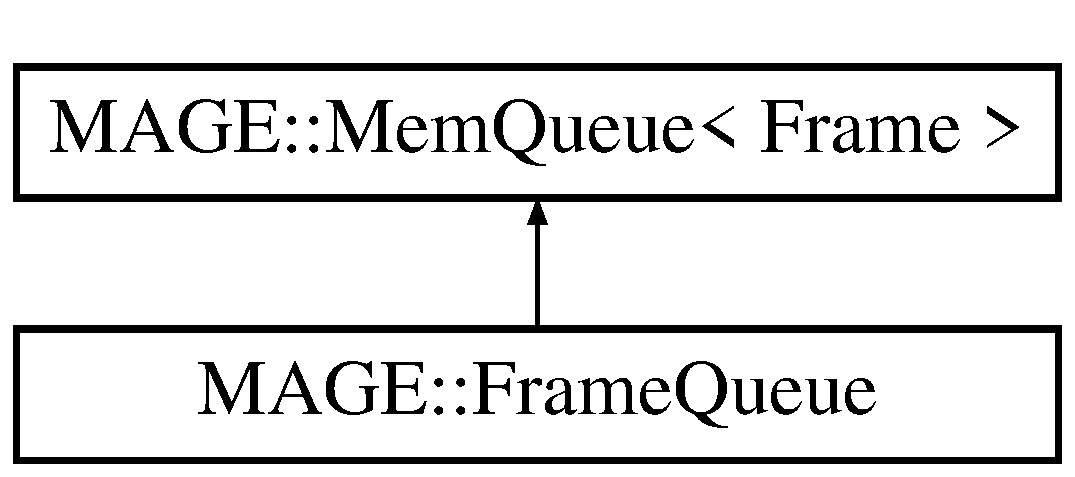
\includegraphics[height=2.000000cm]{class_m_a_g_e_1_1_frame_queue}
\end{center}
\end{figure}
\subsection*{Public Member Functions}
\begin{DoxyCompactItemize}
\item 
\hypertarget{class_m_a_g_e_1_1_frame_queue_ac0e14776a1fff8f7c08680228bf7b928}{{\bfseries Frame\-Queue} (unsigned int queue\-Len)}\label{class_m_a_g_e_1_1_frame_queue_ac0e14776a1fff8f7c08680228bf7b928}

\item 
\hypertarget{class_m_a_g_e_1_1_frame_queue_ad57e61773de705ea155e62f6956fc2f5}{void {\bfseries print\-Queue} (void)}\label{class_m_a_g_e_1_1_frame_queue_ad57e61773de705ea155e62f6956fc2f5}

\end{DoxyCompactItemize}
\subsection*{Additional Inherited Members}


The documentation for this class was generated from the following files\-:\begin{DoxyCompactItemize}
\item 
/\-Users/\-Maipn/\-Documents/my\-Libs/\-M\-A\-G\-E/magelib-\/2.\-00/src/\hyperlink{_frame_queue_8h}{Frame\-Queue.\-h}\item 
/\-Users/\-Maipn/\-Documents/my\-Libs/\-M\-A\-G\-E/magelib-\/2.\-00/src/\hyperlink{_frame_queue_8cpp}{Frame\-Queue.\-cpp}\end{DoxyCompactItemize}

\hypertarget{class_m_a_g_e_1_1_label}{\section{M\-A\-G\-E\-:\-:Label Class Reference}
\label{class_m_a_g_e_1_1_label}\index{M\-A\-G\-E\-::\-Label@{M\-A\-G\-E\-::\-Label}}
}
\subsection*{Public Member Functions}
\begin{DoxyCompactItemize}
\item 
\hypertarget{class_m_a_g_e_1_1_label_a52e386d730501d12817be92f89cb2611}{{\bfseries Label} (string q)}\label{class_m_a_g_e_1_1_label_a52e386d730501d12817be92f89cb2611}

\item 
\hypertarget{class_m_a_g_e_1_1_label_a5fb8ca583cd8ec3beed66640785e29d1}{string {\bfseries get\-Query} (void)}\label{class_m_a_g_e_1_1_label_a5fb8ca583cd8ec3beed66640785e29d1}

\item 
\hypertarget{class_m_a_g_e_1_1_label_a4992f435a3ce7b6aea25e09c5fc31e76}{double {\bfseries get\-Speed} (void)}\label{class_m_a_g_e_1_1_label_a4992f435a3ce7b6aea25e09c5fc31e76}

\item 
\hypertarget{class_m_a_g_e_1_1_label_afc10c4c04c795c4139d53a50f4372446}{int {\bfseries get\-Begin} (void)}\label{class_m_a_g_e_1_1_label_afc10c4c04c795c4139d53a50f4372446}

\item 
\hypertarget{class_m_a_g_e_1_1_label_a1ebed98d1be44acec4b76508ad4aabdc}{int {\bfseries get\-End} (void)}\label{class_m_a_g_e_1_1_label_a1ebed98d1be44acec4b76508ad4aabdc}

\item 
\hypertarget{class_m_a_g_e_1_1_label_aec652c9a05431ed75a93c5166d9760c5}{bool {\bfseries get\-Is\-Forced} (void)}\label{class_m_a_g_e_1_1_label_aec652c9a05431ed75a93c5166d9760c5}

\item 
\hypertarget{class_m_a_g_e_1_1_label_a371dc0984e9a505b06ddd6f750ed251a}{void {\bfseries set\-Query} (string aquery)}\label{class_m_a_g_e_1_1_label_a371dc0984e9a505b06ddd6f750ed251a}

\item 
\hypertarget{class_m_a_g_e_1_1_label_a9ac98d6509ab6e758b9660d2a5aa46ed}{void {\bfseries set\-Begin} (int abegin)}\label{class_m_a_g_e_1_1_label_a9ac98d6509ab6e758b9660d2a5aa46ed}

\item 
\hypertarget{class_m_a_g_e_1_1_label_abd9e189054153f714d6c85b5c50bb1ba}{void {\bfseries set\-End} (int aend)}\label{class_m_a_g_e_1_1_label_abd9e189054153f714d6c85b5c50bb1ba}

\item 
\hypertarget{class_m_a_g_e_1_1_label_ae307a1bd87eac39162ca659d6984e154}{void {\bfseries set\-Speed} (double aspeed)}\label{class_m_a_g_e_1_1_label_ae307a1bd87eac39162ca659d6984e154}

\item 
\hypertarget{class_m_a_g_e_1_1_label_a5e5c9387f04be05ae215bea33db15bbf}{void {\bfseries set\-Is\-Forced} (bool is\-Duration\-Forced)}\label{class_m_a_g_e_1_1_label_a5e5c9387f04be05ae215bea33db15bbf}

\item 
\hypertarget{class_m_a_g_e_1_1_label_adda3f353ba52de2abdf3773ec976875a}{void {\bfseries print\-Query} (void)}\label{class_m_a_g_e_1_1_label_adda3f353ba52de2abdf3773ec976875a}

\item 
\hypertarget{class_m_a_g_e_1_1_label_ab712ec7ae4d3ebf1ab041845da608719}{void {\bfseries parse\-Query} (string q)}\label{class_m_a_g_e_1_1_label_ab712ec7ae4d3ebf1ab041845da608719}

\end{DoxyCompactItemize}
\subsection*{Protected Attributes}
\begin{DoxyCompactItemize}
\item 
\hypertarget{class_m_a_g_e_1_1_label_a2a35d82d85dbe5640121e4e829b59a52}{\hyperlink{class_m_a_g_e_1_1_label_memory}{Label\-Memory} {\bfseries label\-Memory}}\label{class_m_a_g_e_1_1_label_a2a35d82d85dbe5640121e4e829b59a52}

\item 
\hypertarget{class_m_a_g_e_1_1_label_a2d39a9bcadb698c17ff42d4b999faac8}{string {\bfseries query}}\label{class_m_a_g_e_1_1_label_a2d39a9bcadb698c17ff42d4b999faac8}

\item 
\hypertarget{class_m_a_g_e_1_1_label_afec7c4e82578ed9d9b03878107c223df}{bool {\bfseries is\-Forced}}\label{class_m_a_g_e_1_1_label_afec7c4e82578ed9d9b03878107c223df}

\item 
\hypertarget{class_m_a_g_e_1_1_label_a2944a3886038159fd5d5ab0b798fa93b}{double {\bfseries speed}}\label{class_m_a_g_e_1_1_label_a2944a3886038159fd5d5ab0b798fa93b}

\item 
\hypertarget{class_m_a_g_e_1_1_label_abfbfddb7e4e03a69d7e2648c6f78c69a}{int {\bfseries begin}}\label{class_m_a_g_e_1_1_label_abfbfddb7e4e03a69d7e2648c6f78c69a}

\item 
\hypertarget{class_m_a_g_e_1_1_label_a1902501774c298de2f29709b715e7b01}{int {\bfseries end}}\label{class_m_a_g_e_1_1_label_a1902501774c298de2f29709b715e7b01}

\end{DoxyCompactItemize}


The documentation for this class was generated from the following files\-:\begin{DoxyCompactItemize}
\item 
/\-Users/\-Maipn/\-Documents/my\-Libs/\-M\-A\-G\-E/magelib-\/2.\-00/src/\hyperlink{_label_8h}{Label.\-h}\item 
/\-Users/\-Maipn/\-Documents/my\-Libs/\-M\-A\-G\-E/magelib-\/2.\-00/src/\hyperlink{_label_8cpp}{Label.\-cpp}\end{DoxyCompactItemize}

\hypertarget{class_m_a_g_e_1_1_label_memory}{\section{M\-A\-G\-E\-:\-:Label\-Memory Class Reference}
\label{class_m_a_g_e_1_1_label_memory}\index{M\-A\-G\-E\-::\-Label\-Memory@{M\-A\-G\-E\-::\-Label\-Memory}}
}
\subsection*{Public Attributes}
\begin{DoxyCompactItemize}
\item 
\hypertarget{class_m_a_g_e_1_1_label_memory_a623b0a23723b50d2bb7746b015ee8bd5}{char {\bfseries str\-Query} \mbox{[}max\-Str\-Len\mbox{]}}\label{class_m_a_g_e_1_1_label_memory_a623b0a23723b50d2bb7746b015ee8bd5}

\item 
\hypertarget{class_m_a_g_e_1_1_label_memory_a382f808581ccf99a9bb6f8b086005960}{char {\bfseries str\-Begin} \mbox{[}max\-Str\-Len\mbox{]}}\label{class_m_a_g_e_1_1_label_memory_a382f808581ccf99a9bb6f8b086005960}

\item 
\hypertarget{class_m_a_g_e_1_1_label_memory_a9e14137e9d57426d097cf3e266a2f153}{char {\bfseries str\-End} \mbox{[}max\-Str\-Len\mbox{]}}\label{class_m_a_g_e_1_1_label_memory_a9e14137e9d57426d097cf3e266a2f153}

\end{DoxyCompactItemize}


The documentation for this class was generated from the following files\-:\begin{DoxyCompactItemize}
\item 
/\-Users/\-Maipn/\-Documents/my\-Libs/\-M\-A\-G\-E/magelib-\/2.\-00/src/\hyperlink{_label_8h}{Label.\-h}\item 
/\-Users/\-Maipn/\-Documents/my\-Libs/\-M\-A\-G\-E/magelib-\/2.\-00/src/\hyperlink{_label_8cpp}{Label.\-cpp}\end{DoxyCompactItemize}

\hypertarget{class_m_a_g_e_1_1_label_queue}{\section{M\-A\-G\-E\-:\-:Label\-Queue Class Reference}
\label{class_m_a_g_e_1_1_label_queue}\index{M\-A\-G\-E\-::\-Label\-Queue@{M\-A\-G\-E\-::\-Label\-Queue}}
}
\subsection*{Public Member Functions}
\begin{DoxyCompactItemize}
\item 
\hyperlink{class_m_a_g_e_1_1_label_queue_a5d69bbec1eefe9fccd34a14802d18e33}{Label\-Queue} (unsigned int size)
\item 
void \hyperlink{class_m_a_g_e_1_1_label_queue_abd3acda693815cbb59cc3a084d9c0829}{push} (\hyperlink{class_m_a_g_e_1_1_label}{Label} \&label)
\item 
void \hyperlink{class_m_a_g_e_1_1_label_queue_afc70a0500860585adbd8924c8d56b956}{push} (void)
\item 
void \hyperlink{class_m_a_g_e_1_1_label_queue_a096711daf22ea9b75b2049f2be70aea3}{pop} (\hyperlink{class_m_a_g_e_1_1_label}{Label} \&label)
\item 
void \hyperlink{class_m_a_g_e_1_1_label_queue_a71ab29606a69856b6d3a6015267e31d7}{pop} (void)
\item 
void \hyperlink{class_m_a_g_e_1_1_label_queue_a1adf91ffe03fdcf9b1746e4003b21c51}{get} (\hyperlink{class_m_a_g_e_1_1_label}{Label} \&label)
\item 
\hyperlink{class_m_a_g_e_1_1_label}{Label} $\ast$ \hyperlink{class_m_a_g_e_1_1_label_queue_aa6ac0d09888731bd508e63bb0230297a}{get} (void)
\item 
\hyperlink{class_m_a_g_e_1_1_label}{Label} $\ast$ \hyperlink{class_m_a_g_e_1_1_label_queue_ad601c5c5034dd42fbbe511d4fb715b56}{next} (void)
\item 
\hypertarget{class_m_a_g_e_1_1_label_queue_a0fcea608643f081bd3044706ae98142d}{void {\bfseries print} (void)}\label{class_m_a_g_e_1_1_label_queue_a0fcea608643f081bd3044706ae98142d}

\item 
bool \hyperlink{class_m_a_g_e_1_1_label_queue_a0a2d45cf42d8ba62240d544b61f690c8}{is\-Empty} (void)
\item 
bool \hyperlink{class_m_a_g_e_1_1_label_queue_ac55a268122abcec371db89ecacdfd94e}{is\-Full} (void)
\end{DoxyCompactItemize}
\subsection*{Protected Attributes}
\begin{DoxyCompactItemize}
\item 
\hypertarget{class_m_a_g_e_1_1_label_queue_ac3e06511af7d94f1eeff2911fff27325}{vector$<$ \hyperlink{class_m_a_g_e_1_1_label}{Label} $>$ {\bfseries queue}}\label{class_m_a_g_e_1_1_label_queue_ac3e06511af7d94f1eeff2911fff27325}

\item 
\hypertarget{class_m_a_g_e_1_1_label_queue_afa43057433f1ab70f910d74930e55a6e}{unsigned int {\bfseries read}}\label{class_m_a_g_e_1_1_label_queue_afa43057433f1ab70f910d74930e55a6e}

\item 
\hypertarget{class_m_a_g_e_1_1_label_queue_a0618d5991d8d4541dbf1cd208998d2f2}{unsigned int {\bfseries write}}\label{class_m_a_g_e_1_1_label_queue_a0618d5991d8d4541dbf1cd208998d2f2}

\item 
\hypertarget{class_m_a_g_e_1_1_label_queue_aeb3e11635459ef045c4b93966775d723}{unsigned int {\bfseries n\-Of\-Labels}}\label{class_m_a_g_e_1_1_label_queue_aeb3e11635459ef045c4b93966775d723}

\end{DoxyCompactItemize}


\subsection{Constructor \& Destructor Documentation}
\hypertarget{class_m_a_g_e_1_1_label_queue_a5d69bbec1eefe9fccd34a14802d18e33}{\index{M\-A\-G\-E\-::\-Label\-Queue@{M\-A\-G\-E\-::\-Label\-Queue}!Label\-Queue@{Label\-Queue}}
\index{Label\-Queue@{Label\-Queue}!MAGE::LabelQueue@{M\-A\-G\-E\-::\-Label\-Queue}}
\subsubsection[{Label\-Queue}]{\setlength{\rightskip}{0pt plus 5cm}M\-A\-G\-E\-::\-Label\-Queue\-::\-Label\-Queue (
\begin{DoxyParamCaption}
\item[{unsigned int}]{size}
\end{DoxyParamCaption}
)}}\label{class_m_a_g_e_1_1_label_queue_a5d69bbec1eefe9fccd34a14802d18e33}

\begin{DoxyParams}{Parameters}
{\em size} & max size of the \hyperlink{class_m_a_g_e_1_1_label_queue}{Label\-Queue}. i.\-e. how many \hyperlink{class_m_a_g_e_1_1_label}{Label} the buffer ring can contain before it's full. \\
\hline
\end{DoxyParams}


\subsection{Member Function Documentation}
\hypertarget{class_m_a_g_e_1_1_label_queue_a1adf91ffe03fdcf9b1746e4003b21c51}{\index{M\-A\-G\-E\-::\-Label\-Queue@{M\-A\-G\-E\-::\-Label\-Queue}!get@{get}}
\index{get@{get}!MAGE::LabelQueue@{M\-A\-G\-E\-::\-Label\-Queue}}
\subsubsection[{get}]{\setlength{\rightskip}{0pt plus 5cm}void M\-A\-G\-E\-::\-Label\-Queue\-::get (
\begin{DoxyParamCaption}
\item[{{\bf Label} \&}]{label}
\end{DoxyParamCaption}
)}}\label{class_m_a_g_e_1_1_label_queue_a1adf91ffe03fdcf9b1746e4003b21c51}
like \hyperlink{class_m_a_g_e_1_1_label_queue_a096711daf22ea9b75b2049f2be70aea3}{pop(\-Label\&)} but does not advance in the queue \hypertarget{class_m_a_g_e_1_1_label_queue_aa6ac0d09888731bd508e63bb0230297a}{\index{M\-A\-G\-E\-::\-Label\-Queue@{M\-A\-G\-E\-::\-Label\-Queue}!get@{get}}
\index{get@{get}!MAGE::LabelQueue@{M\-A\-G\-E\-::\-Label\-Queue}}
\subsubsection[{get}]{\setlength{\rightskip}{0pt plus 5cm}{\bf M\-A\-G\-E\-::\-Label} $\ast$ M\-A\-G\-E\-::\-Label\-Queue\-::get (
\begin{DoxyParamCaption}
\item[{void}]{}
\end{DoxyParamCaption}
)}}\label{class_m_a_g_e_1_1_label_queue_aa6ac0d09888731bd508e63bb0230297a}
Access the oldest item of the F\-I\-F\-O queue. This is meant to be used with \hyperlink{class_m_a_g_e_1_1_label_queue_a71ab29606a69856b6d3a6015267e31d7}{pop(void)}. See \hyperlink{class_m_a_g_e_1_1_label_queue_a71ab29606a69856b6d3a6015267e31d7}{pop(void)} doc for more complete explanation

\begin{DoxyReturn}{Returns}
a pointer to the item of the queue that \hyperlink{class_m_a_g_e_1_1_label_queue_a71ab29606a69856b6d3a6015267e31d7}{pop()} would remove. i.\-e. the oldest slot in the F\-I\-F\-O 
\end{DoxyReturn}
\hypertarget{class_m_a_g_e_1_1_label_queue_a0a2d45cf42d8ba62240d544b61f690c8}{\index{M\-A\-G\-E\-::\-Label\-Queue@{M\-A\-G\-E\-::\-Label\-Queue}!is\-Empty@{is\-Empty}}
\index{is\-Empty@{is\-Empty}!MAGE::LabelQueue@{M\-A\-G\-E\-::\-Label\-Queue}}
\subsubsection[{is\-Empty}]{\setlength{\rightskip}{0pt plus 5cm}bool M\-A\-G\-E\-::\-Label\-Queue\-::is\-Empty (
\begin{DoxyParamCaption}
\item[{void}]{}
\end{DoxyParamCaption}
)}}\label{class_m_a_g_e_1_1_label_queue_a0a2d45cf42d8ba62240d544b61f690c8}
\begin{DoxyReturn}{Returns}
true if the queue is empty, false otherwise 
\end{DoxyReturn}
\hypertarget{class_m_a_g_e_1_1_label_queue_ac55a268122abcec371db89ecacdfd94e}{\index{M\-A\-G\-E\-::\-Label\-Queue@{M\-A\-G\-E\-::\-Label\-Queue}!is\-Full@{is\-Full}}
\index{is\-Full@{is\-Full}!MAGE::LabelQueue@{M\-A\-G\-E\-::\-Label\-Queue}}
\subsubsection[{is\-Full}]{\setlength{\rightskip}{0pt plus 5cm}bool M\-A\-G\-E\-::\-Label\-Queue\-::is\-Full (
\begin{DoxyParamCaption}
\item[{void}]{}
\end{DoxyParamCaption}
)}}\label{class_m_a_g_e_1_1_label_queue_ac55a268122abcec371db89ecacdfd94e}
\begin{DoxyReturn}{Returns}
true if the queue is full, i.\-e. if it contains the max number of elements given to the constructor, false otherwise 
\end{DoxyReturn}
\hypertarget{class_m_a_g_e_1_1_label_queue_ad601c5c5034dd42fbbe511d4fb715b56}{\index{M\-A\-G\-E\-::\-Label\-Queue@{M\-A\-G\-E\-::\-Label\-Queue}!next@{next}}
\index{next@{next}!MAGE::LabelQueue@{M\-A\-G\-E\-::\-Label\-Queue}}
\subsubsection[{next}]{\setlength{\rightskip}{0pt plus 5cm}{\bf M\-A\-G\-E\-::\-Label} $\ast$ M\-A\-G\-E\-::\-Label\-Queue\-::next (
\begin{DoxyParamCaption}
\item[{void}]{}
\end{DoxyParamCaption}
)}}\label{class_m_a_g_e_1_1_label_queue_ad601c5c5034dd42fbbe511d4fb715b56}
Access next available slot of the memory pool. This is meant to be used with \hyperlink{class_m_a_g_e_1_1_label_queue_afc70a0500860585adbd8924c8d56b956}{push(void)}. see \hyperlink{class_m_a_g_e_1_1_label_queue_afc70a0500860585adbd8924c8d56b956}{push(void)} doc for more complete explanations.

\begin{DoxyReturn}{Returns}
a pointer to the item of the queue that \hyperlink{class_m_a_g_e_1_1_label_queue_afc70a0500860585adbd8924c8d56b956}{push()} would write to. i.\-e. the next available slot in memory that has not yet been pushed into the F\-I\-F\-O 
\end{DoxyReturn}
\hypertarget{class_m_a_g_e_1_1_label_queue_a096711daf22ea9b75b2049f2be70aea3}{\index{M\-A\-G\-E\-::\-Label\-Queue@{M\-A\-G\-E\-::\-Label\-Queue}!pop@{pop}}
\index{pop@{pop}!MAGE::LabelQueue@{M\-A\-G\-E\-::\-Label\-Queue}}
\subsubsection[{pop}]{\setlength{\rightskip}{0pt plus 5cm}void M\-A\-G\-E\-::\-Label\-Queue\-::pop (
\begin{DoxyParamCaption}
\item[{{\bf Label} \&}]{label}
\end{DoxyParamCaption}
)}}\label{class_m_a_g_e_1_1_label_queue_a096711daf22ea9b75b2049f2be70aea3}
remove the oldest item in the queue


\begin{DoxyParams}{Parameters}
{\em label} & an instance of \hyperlink{class_m_a_g_e_1_1_label}{M\-A\-G\-E\-::\-Label} into which the \hyperlink{class_m_a_g_e_1_1_label_queue_a71ab29606a69856b6d3a6015267e31d7}{pop()}'d label will be copied before being removed from the queue \\
\hline
\end{DoxyParams}
\hypertarget{class_m_a_g_e_1_1_label_queue_a71ab29606a69856b6d3a6015267e31d7}{\index{M\-A\-G\-E\-::\-Label\-Queue@{M\-A\-G\-E\-::\-Label\-Queue}!pop@{pop}}
\index{pop@{pop}!MAGE::LabelQueue@{M\-A\-G\-E\-::\-Label\-Queue}}
\subsubsection[{pop}]{\setlength{\rightskip}{0pt plus 5cm}void M\-A\-G\-E\-::\-Label\-Queue\-::pop (
\begin{DoxyParamCaption}
\item[{void}]{}
\end{DoxyParamCaption}
)}}\label{class_m_a_g_e_1_1_label_queue_a71ab29606a69856b6d3a6015267e31d7}
remove the oldest item in the queue. In this case, there is no copy of a label, instead the 'read' pointer that points to the oldest item in the queue is incremented to the next item of the queue and the item previously pointed to is returned into the memory pool. Usage is in 3 steps which could be summarized into \char`\"{}access, read, delete\char`\"{}\-:

\hyperlink{class_m_a_g_e_1_1_label}{Label} $\ast$label = label\-Queue-\/$>$\hyperlink{class_m_a_g_e_1_1_label_queue_aa6ac0d09888731bd508e63bb0230297a}{get()};//access oldest item in the queue string s = label-\/$>$get\-Query();//read it, use it, ... label\-Queue-\/$>$\hyperlink{class_m_a_g_e_1_1_label_queue_a71ab29606a69856b6d3a6015267e31d7}{pop()};//remove it from the queue (advance 'read' pointer) //never do this after a \hyperlink{class_m_a_g_e_1_1_label_queue_a71ab29606a69856b6d3a6015267e31d7}{pop()} \-: string s2 = label-\/$>$get\-Query();//don't do this

Note that once \hyperlink{class_m_a_g_e_1_1_label_queue_a71ab29606a69856b6d3a6015267e31d7}{pop()} has been called, the item can be overwritten at any time by a subsequent \hyperlink{class_m_a_g_e_1_1_label_queue_ad601c5c5034dd42fbbe511d4fb715b56}{next()}/push(). Therefore if the \hyperlink{class_m_a_g_e_1_1_label}{Label} has to be used but without blocking/clogging up the queue, it is better to make a copy-\/pop() with \hyperlink{class_m_a_g_e_1_1_label_queue_a096711daf22ea9b75b2049f2be70aea3}{pop(\-Label\&)}

\hyperlink{class_m_a_g_e_1_1_label}{Label} $\ast$label = label\-Queue-\/$>$\hyperlink{class_m_a_g_e_1_1_label_queue_aa6ac0d09888731bd508e63bb0230297a}{get()};//access oldest item in the queue label\-Queue-\/$>$\hyperlink{class_m_a_g_e_1_1_label_queue_a71ab29606a69856b6d3a6015267e31d7}{pop()};//remove it from the queue (advance 'read' pointer) //never do this after a \hyperlink{class_m_a_g_e_1_1_label_queue_a71ab29606a69856b6d3a6015267e31d7}{pop()} \-: string s = label-\/$>$get\-Query();//don't do this

//do this instead \hyperlink{class_m_a_g_e_1_1_label}{Label} label; label\-Queue-\/$>$pop(label);//remove it from the queue (advance 'read' pointer) string s = label.\-get\-Query();//label is a local copy of the label that has been \hyperlink{class_m_a_g_e_1_1_label_queue_a71ab29606a69856b6d3a6015267e31d7}{pop()}'d \hypertarget{class_m_a_g_e_1_1_label_queue_abd3acda693815cbb59cc3a084d9c0829}{\index{M\-A\-G\-E\-::\-Label\-Queue@{M\-A\-G\-E\-::\-Label\-Queue}!push@{push}}
\index{push@{push}!MAGE::LabelQueue@{M\-A\-G\-E\-::\-Label\-Queue}}
\subsubsection[{push}]{\setlength{\rightskip}{0pt plus 5cm}void M\-A\-G\-E\-::\-Label\-Queue\-::push (
\begin{DoxyParamCaption}
\item[{{\bf Label} \&}]{label}
\end{DoxyParamCaption}
)}}\label{class_m_a_g_e_1_1_label_queue_abd3acda693815cbb59cc3a084d9c0829}
push a new \hyperlink{class_m_a_g_e_1_1_label}{M\-A\-G\-E\-::\-Label} into the F\-I\-F\-O queue by copying it.


\begin{DoxyParams}{Parameters}
{\em label} & an instance of \hyperlink{class_m_a_g_e_1_1_label}{M\-A\-G\-E\-::\-Label} that will be copied into the youngest item of the memory queue \\
\hline
\end{DoxyParams}
\hypertarget{class_m_a_g_e_1_1_label_queue_afc70a0500860585adbd8924c8d56b956}{\index{M\-A\-G\-E\-::\-Label\-Queue@{M\-A\-G\-E\-::\-Label\-Queue}!push@{push}}
\index{push@{push}!MAGE::LabelQueue@{M\-A\-G\-E\-::\-Label\-Queue}}
\subsubsection[{push}]{\setlength{\rightskip}{0pt plus 5cm}void M\-A\-G\-E\-::\-Label\-Queue\-::push (
\begin{DoxyParamCaption}
\item[{void}]{}
\end{DoxyParamCaption}
)}}\label{class_m_a_g_e_1_1_label_queue_afc70a0500860585adbd8924c8d56b956}
push a new \hyperlink{class_m_a_g_e_1_1_label}{M\-A\-G\-E\-::\-Label} into the F\-I\-F\-O queue. In this case, there is no copy of a label, instead the next slot of the memory pool is added to the queue. It is supposed that said slot has been accessed with \hyperlink{class_m_a_g_e_1_1_label_queue_ad601c5c5034dd42fbbe511d4fb715b56}{next()} and modified beforehand. Usage is in 3 steps which could be summarized into \char`\"{}access, write, save\char`\"{}\-:

\hyperlink{class_m_a_g_e_1_1_label}{Label} $\ast$label = label\-Queue-\/$>$\hyperlink{class_m_a_g_e_1_1_label_queue_ad601c5c5034dd42fbbe511d4fb715b56}{next()};//access next memory slot label-\/$>$set\-Query(\char`\"{}ae$^\wedge$l-\/ax+s=w@...\char`\"{});//modify it label\-Queue-\/$>$\hyperlink{class_m_a_g_e_1_1_label_queue_afc70a0500860585adbd8924c8d56b956}{push()};//save it into the queue (advance 'write' pointer) 

The documentation for this class was generated from the following files\-:\begin{DoxyCompactItemize}
\item 
/\-Users/\-Maipn/\-Documents/my\-Libs/\-M\-A\-G\-E/magelib-\/2.\-00/src/\hyperlink{_label_queue_8h}{Label\-Queue.\-h}\item 
/\-Users/\-Maipn/\-Documents/my\-Libs/\-M\-A\-G\-E/magelib-\/2.\-00/src/\hyperlink{_label_queue_8cpp}{Label\-Queue.\-cpp}\end{DoxyCompactItemize}

\hypertarget{class_m_a_g_e_1_1_mage}{\section{M\-A\-G\-E\-:\-:Mage Class Reference}
\label{class_m_a_g_e_1_1_mage}\index{M\-A\-G\-E\-::\-Mage@{M\-A\-G\-E\-::\-Mage}}
}
\subsection*{Public Member Functions}
\begin{DoxyCompactItemize}
\item 
\hypertarget{class_m_a_g_e_1_1_mage_addc8c5637cd9e1c38b077354bd89da33}{{\bfseries Mage} (std\-::string Engine\-Name, int argc, char $\ast$$\ast$argv)}\label{class_m_a_g_e_1_1_mage_addc8c5637cd9e1c38b077354bd89da33}

\item 
\hypertarget{class_m_a_g_e_1_1_mage_a5c50ae1e8e7384c88912035efa47af4d}{{\bfseries Mage} (std\-::string Engine\-Name, std\-::string conf\-Filename)}\label{class_m_a_g_e_1_1_mage_a5c50ae1e8e7384c88912035efa47af4d}

\item 
\hypertarget{class_m_a_g_e_1_1_mage_ae8ea8a1afdb6a62f0813b4bdadc25281}{\hyperlink{struct_m_a_g_e_1_1_frame}{Frame} {\bfseries get\-Frame} (void)}\label{class_m_a_g_e_1_1_mage_ae8ea8a1afdb6a62f0813b4bdadc25281}

\item 
\hypertarget{class_m_a_g_e_1_1_mage_ac1e3d8167214d6e3f4738981a4d5e36d}{\hyperlink{class_m_a_g_e_1_1_label}{Label} {\bfseries get\-Label} (void)}\label{class_m_a_g_e_1_1_mage_ac1e3d8167214d6e3f4738981a4d5e36d}

\item 
\hypertarget{class_m_a_g_e_1_1_mage_a5a5c3797369cb5a8a8f65aeed98c94a1}{\hyperlink{class_m_a_g_e_1_1_model}{Model} $\ast$ {\bfseries get\-Model} (void)}\label{class_m_a_g_e_1_1_mage_a5a5c3797369cb5a8a8f65aeed98c94a1}

\item 
\hypertarget{class_m_a_g_e_1_1_mage_a1d0b5e7d42b9a72d53e3d9bcd853f12b}{\hyperlink{class_m_a_g_e_1_1_vocoder}{Vocoder} $\ast$ {\bfseries get\-Vocoder} (void)}\label{class_m_a_g_e_1_1_mage_a1d0b5e7d42b9a72d53e3d9bcd853f12b}

\item 
\hypertarget{class_m_a_g_e_1_1_mage_a8f02241895387ecd266748e6c8c54cde}{\hyperlink{class_m_a_g_e_1_1_label_queue}{Label\-Queue} $\ast$ {\bfseries get\-Label\-Queue} (void)}\label{class_m_a_g_e_1_1_mage_a8f02241895387ecd266748e6c8c54cde}

\item 
\hypertarget{class_m_a_g_e_1_1_mage_ac87e1ff7eb1a77a058a3e0c1c586128b}{\hyperlink{class_m_a_g_e_1_1_model_queue}{Model\-Queue} $\ast$ {\bfseries get\-Model\-Queue} (void)}\label{class_m_a_g_e_1_1_mage_ac87e1ff7eb1a77a058a3e0c1c586128b}

\item 
\hypertarget{class_m_a_g_e_1_1_mage_afb485148201b8bf80a323cc0337e5b7b}{\hyperlink{class_m_a_g_e_1_1_frame_queue}{Frame\-Queue} $\ast$ {\bfseries get\-Frame\-Queue} (void)}\label{class_m_a_g_e_1_1_mage_afb485148201b8bf80a323cc0337e5b7b}

\item 
\hypertarget{class_m_a_g_e_1_1_mage_ae150f208260289625610d6d8c1d99b8b}{int {\bfseries get\-Sample\-Counter} (void)}\label{class_m_a_g_e_1_1_mage_ae150f208260289625610d6d8c1d99b8b}

\item 
\hypertarget{class_m_a_g_e_1_1_mage_ab236f986ba28ec053d142be80697892e}{double {\bfseries get\-Speed} (void)}\label{class_m_a_g_e_1_1_mage_ab236f986ba28ec053d142be80697892e}

\item 
\hypertarget{class_m_a_g_e_1_1_mage_ace06f1944bb05f005772b6e83b5407ef}{double {\bfseries get\-Label\-Speed} (void)}\label{class_m_a_g_e_1_1_mage_ace06f1944bb05f005772b6e83b5407ef}

\item 
\hypertarget{class_m_a_g_e_1_1_mage_aef955527c26da647594a51f6a8d9888d}{std\-::string {\bfseries get\-Default\-Engine} (void)}\label{class_m_a_g_e_1_1_mage_aef955527c26da647594a51f6a8d9888d}

\item 
\hypertarget{class_m_a_g_e_1_1_mage_a756095e0c9f07afa5d7bc0569a0f93d5}{double {\bfseries get\-Pitch} (void)}\label{class_m_a_g_e_1_1_mage_a756095e0c9f07afa5d7bc0569a0f93d5}

\item 
\hypertarget{class_m_a_g_e_1_1_mage_a1b2b4ac762d9975341f1dda039d6063e}{double {\bfseries get\-Alpha} (void)}\label{class_m_a_g_e_1_1_mage_a1b2b4ac762d9975341f1dda039d6063e}

\item 
\hypertarget{class_m_a_g_e_1_1_mage_a26952851fc21f3b39f7c88729a6b4ea8}{double {\bfseries get\-Gamma} (void)}\label{class_m_a_g_e_1_1_mage_a26952851fc21f3b39f7c88729a6b4ea8}

\item 
\hypertarget{class_m_a_g_e_1_1_mage_a9a3c9ba41daa6de0d7fa8295873da3ab}{double {\bfseries get\-P\-Order} (void)}\label{class_m_a_g_e_1_1_mage_a9a3c9ba41daa6de0d7fa8295873da3ab}

\item 
\hypertarget{class_m_a_g_e_1_1_mage_ab2d2a99d80b9e44fb31edc013acf10c2}{double {\bfseries get\-Volume} (void)}\label{class_m_a_g_e_1_1_mage_ab2d2a99d80b9e44fb31edc013acf10c2}

\item 
\hypertarget{class_m_a_g_e_1_1_mage_a82621924af342fa5aeee62a75491b3cc}{double {\bfseries get\-Duration} (void)}\label{class_m_a_g_e_1_1_mage_a82621924af342fa5aeee62a75491b3cc}

\item 
\hypertarget{class_m_a_g_e_1_1_mage_ac7bf18d62123a16be7062332ff9e4199}{void {\bfseries set\-Frame} (\hyperlink{struct_m_a_g_e_1_1_frame}{Frame} aframe)}\label{class_m_a_g_e_1_1_mage_ac7bf18d62123a16be7062332ff9e4199}

\item 
\hypertarget{class_m_a_g_e_1_1_mage_aec2890ec81154a590c43771fcbc5c01f}{void {\bfseries set\-Label} (\hyperlink{class_m_a_g_e_1_1_label}{Label} alabel)}\label{class_m_a_g_e_1_1_mage_aec2890ec81154a590c43771fcbc5c01f}

\item 
\hypertarget{class_m_a_g_e_1_1_mage_a5b5483ba34fdc6fe9c8f120737ad8e5f}{void {\bfseries set\-Model} (\hyperlink{class_m_a_g_e_1_1_model}{Model} $\ast$amodel)}\label{class_m_a_g_e_1_1_mage_a5b5483ba34fdc6fe9c8f120737ad8e5f}

\item 
\hypertarget{class_m_a_g_e_1_1_mage_a40e130dd62fecb5039f1228b6bdc2464}{void {\bfseries set\-Vocoder} (\hyperlink{class_m_a_g_e_1_1_vocoder}{Vocoder} $\ast$avocoder)}\label{class_m_a_g_e_1_1_mage_a40e130dd62fecb5039f1228b6bdc2464}

\item 
\hypertarget{class_m_a_g_e_1_1_mage_a7f8dabb44a06ecee3abde35842ffe48e}{void {\bfseries set\-Label\-Speed} (double a\-Label\-Speed)}\label{class_m_a_g_e_1_1_mage_a7f8dabb44a06ecee3abde35842ffe48e}

\item 
\hypertarget{class_m_a_g_e_1_1_mage_a9b17d63eb3d7e5056fc1e07341abe15a}{void {\bfseries set\-Label\-Queue} (\hyperlink{class_m_a_g_e_1_1_label_queue}{Label\-Queue} $\ast$alabel\-Queue)}\label{class_m_a_g_e_1_1_mage_a9b17d63eb3d7e5056fc1e07341abe15a}

\item 
\hypertarget{class_m_a_g_e_1_1_mage_ab2035e9b0d1ba9b37487f8d89933c61a}{void {\bfseries set\-Model\-Queue} (\hyperlink{class_m_a_g_e_1_1_model_queue}{Model\-Queue} $\ast$amodel\-Queue)}\label{class_m_a_g_e_1_1_mage_ab2035e9b0d1ba9b37487f8d89933c61a}

\item 
\hypertarget{class_m_a_g_e_1_1_mage_a150ae12ed4e3ffc3a62abaf5fdfd9e3d}{void {\bfseries set\-Frame\-Queue} (\hyperlink{class_m_a_g_e_1_1_frame_queue}{Frame\-Queue} $\ast$aframe\-Queue)}\label{class_m_a_g_e_1_1_mage_a150ae12ed4e3ffc3a62abaf5fdfd9e3d}

\item 
\hypertarget{class_m_a_g_e_1_1_mage_aa5bcce5e56cc246c7dce73d287d59c9d}{void {\bfseries set\-Alpha} (double alpha)}\label{class_m_a_g_e_1_1_mage_aa5bcce5e56cc246c7dce73d287d59c9d}

\item 
\hypertarget{class_m_a_g_e_1_1_mage_aa619158500973cb5cb30b5017cf4624f}{void {\bfseries set\-Gamma} (double gamma)}\label{class_m_a_g_e_1_1_mage_aa619158500973cb5cb30b5017cf4624f}

\item 
\hypertarget{class_m_a_g_e_1_1_mage_a55ed47d0fcf247afc9dd3d613782ac66}{void {\bfseries set\-P\-Order} (double glitch)}\label{class_m_a_g_e_1_1_mage_a55ed47d0fcf247afc9dd3d613782ac66}

\item 
\hypertarget{class_m_a_g_e_1_1_mage_a1e87dd6829eeb4e5d0877e846b1e7329}{void {\bfseries set\-Volume} (double volume)}\label{class_m_a_g_e_1_1_mage_a1e87dd6829eeb4e5d0877e846b1e7329}

\item 
\hypertarget{class_m_a_g_e_1_1_mage_ae3dd0c90ccb3a22f0bf87347177b4ad3}{void {\bfseries set\-Pitch} (double pitch, int aaction)}\label{class_m_a_g_e_1_1_mage_ae3dd0c90ccb3a22f0bf87347177b4ad3}

\item 
\hypertarget{class_m_a_g_e_1_1_mage_a4002ab5e2dd124e10f8a46713f43bf15}{void {\bfseries set\-Speed} (double aspeed, int aaction)}\label{class_m_a_g_e_1_1_mage_a4002ab5e2dd124e10f8a46713f43bf15}

\item 
\hypertarget{class_m_a_g_e_1_1_mage_aafa5e062b14d856d4ad845dcab706005}{void {\bfseries set\-Duration} (double $\ast$update\-Function, int action)}\label{class_m_a_g_e_1_1_mage_aafa5e062b14d856d4ad845dcab706005}

\item 
\hypertarget{class_m_a_g_e_1_1_mage_ab2cc4ec66c1c570fd70313384406e742}{void {\bfseries set\-Default\-Engine} (std\-::string adefault\-Engine)}\label{class_m_a_g_e_1_1_mage_ab2cc4ec66c1c570fd70313384406e742}

\item 
\hypertarget{class_m_a_g_e_1_1_mage_adef698d2640dc3c76c6faa7c0c9853a9}{void {\bfseries set\-Interpolation\-Functions} (std\-::map$<$ std\-::string, double $\ast$ $>$ ainterpolation\-Functions\-Set)}\label{class_m_a_g_e_1_1_mage_adef698d2640dc3c76c6faa7c0c9853a9}

\item 
\hypertarget{class_m_a_g_e_1_1_mage_acf48640f37d4a797a285930b8e2639be}{double {\bfseries pop\-Samples} (void)}\label{class_m_a_g_e_1_1_mage_acf48640f37d4a797a285930b8e2639be}

\item 
\hypertarget{class_m_a_g_e_1_1_mage_afccd7f699d3a3c95decb77b872642ebd}{bool {\bfseries pop\-Label} (void)}\label{class_m_a_g_e_1_1_mage_afccd7f699d3a3c95decb77b872642ebd}

\item 
\hypertarget{class_m_a_g_e_1_1_mage_af4813e05a1a6390a280302588b7ab84a}{void {\bfseries run} (void)}\label{class_m_a_g_e_1_1_mage_af4813e05a1a6390a280302588b7ab84a}

\item 
\hypertarget{class_m_a_g_e_1_1_mage_a41a3d6bdc9dec7fb502f5d2f3212d95b}{void {\bfseries reset} (void)}\label{class_m_a_g_e_1_1_mage_a41a3d6bdc9dec7fb502f5d2f3212d95b}

\item 
\hypertarget{class_m_a_g_e_1_1_mage_afa6d88eb37afdaf56a762b47df0f3f7c}{void {\bfseries reset\-Vocoder} (void)}\label{class_m_a_g_e_1_1_mage_afa6d88eb37afdaf56a762b47df0f3f7c}

\item 
\hypertarget{class_m_a_g_e_1_1_mage_a7a123427ef52c6e54aa0ebfa3a62d131}{void {\bfseries prepare\-Model} (void)}\label{class_m_a_g_e_1_1_mage_a7a123427ef52c6e54aa0ebfa3a62d131}

\item 
\hypertarget{class_m_a_g_e_1_1_mage_a31c05688b6f303a45f25cecd0d402b6d}{void {\bfseries update\-Samples} (void)}\label{class_m_a_g_e_1_1_mage_a31c05688b6f303a45f25cecd0d402b6d}

\item 
\hypertarget{class_m_a_g_e_1_1_mage_a654955584a96562c1b863b386298444d}{void {\bfseries compute\-Duration} (void)}\label{class_m_a_g_e_1_1_mage_a654955584a96562c1b863b386298444d}

\item 
\hypertarget{class_m_a_g_e_1_1_mage_ad4a3a580d66430a68d8fb27534543eb1}{void {\bfseries compute\-Parameters} (void)}\label{class_m_a_g_e_1_1_mage_ad4a3a580d66430a68d8fb27534543eb1}

\item 
\hypertarget{class_m_a_g_e_1_1_mage_ad1608921d3634dbcedf7ab06eb558b6f}{void {\bfseries optimize\-Parameters} (void)}\label{class_m_a_g_e_1_1_mage_ad1608921d3634dbcedf7ab06eb558b6f}

\item 
\hypertarget{class_m_a_g_e_1_1_mage_ad690491113171be438989d5b070f384b}{void {\bfseries check\-Interpolation\-Weights} (bool forced=false)}\label{class_m_a_g_e_1_1_mage_ad690491113171be438989d5b070f384b}

\item 
\hypertarget{class_m_a_g_e_1_1_mage_a09eeea43ffba1519cb5709f39ddda43b}{void {\bfseries push\-Label} (\hyperlink{class_m_a_g_e_1_1_label}{Label} label)}\label{class_m_a_g_e_1_1_mage_a09eeea43ffba1519cb5709f39ddda43b}

\item 
\hypertarget{class_m_a_g_e_1_1_mage_a44e46eaece0747f143196739223e0435}{void {\bfseries add\-Engine} (std\-::string name, int argc, char $\ast$$\ast$argv)}\label{class_m_a_g_e_1_1_mage_a44e46eaece0747f143196739223e0435}

\item 
\hypertarget{class_m_a_g_e_1_1_mage_a843579b3a69417dc17378feb7b965848}{void {\bfseries add\-Engine} (std\-::string name, std\-::string conf\-Filename)}\label{class_m_a_g_e_1_1_mage_a843579b3a69417dc17378feb7b965848}

\item 
\hypertarget{class_m_a_g_e_1_1_mage_aa374565aaed67cb05b39516e11eb6638}{void {\bfseries remove\-Engine} (std\-::string Engine\-Name)}\label{class_m_a_g_e_1_1_mage_aa374565aaed67cb05b39516e11eb6638}

\item 
\hypertarget{class_m_a_g_e_1_1_mage_a082da9f9d38a4d65029d0d700b52405c}{void {\bfseries enable\-Interpolation} (bool ainterpolation\-Flag)}\label{class_m_a_g_e_1_1_mage_a082da9f9d38a4d65029d0d700b52405c}

\item 
\hypertarget{class_m_a_g_e_1_1_mage_a925cd537c72cd98e1ed488398ad46e45}{void {\bfseries print} (void)}\label{class_m_a_g_e_1_1_mage_a925cd537c72cd98e1ed488398ad46e45}

\end{DoxyCompactItemize}
\subsection*{Protected Attributes}
\begin{DoxyCompactItemize}
\item 
\hypertarget{class_m_a_g_e_1_1_mage_a0bc721d13c832f77794dfbe8446d4ad1}{\hyperlink{class_m_a_g_e_1_1_label_queue}{Label\-Queue} $\ast$ {\bfseries label\-Queue}}\label{class_m_a_g_e_1_1_mage_a0bc721d13c832f77794dfbe8446d4ad1}

\item 
\hypertarget{class_m_a_g_e_1_1_mage_a2a13c60d4174db48bd1b2de2f1f606ed}{\hyperlink{class_m_a_g_e_1_1_model_queue}{Model\-Queue} $\ast$ {\bfseries model\-Queue}}\label{class_m_a_g_e_1_1_mage_a2a13c60d4174db48bd1b2de2f1f606ed}

\item 
\hypertarget{class_m_a_g_e_1_1_mage_a6972a9650e11f8f0e1f28fdb979a8b7c}{\hyperlink{class_m_a_g_e_1_1_frame_queue}{Frame\-Queue} $\ast$ {\bfseries frame\-Queue}}\label{class_m_a_g_e_1_1_mage_a6972a9650e11f8f0e1f28fdb979a8b7c}

\item 
\hypertarget{class_m_a_g_e_1_1_mage_a2cda1c9bd936a2aae08f16048f8a3d8d}{std\-::map$<$ std\-::string, \\*
std\-::pair$<$ double $\ast$, \hyperlink{class_m_a_g_e_1_1_engine}{Engine} $\ast$ $>$ $>$ {\bfseries engine}}\label{class_m_a_g_e_1_1_mage_a2cda1c9bd936a2aae08f16048f8a3d8d}

\item 
\hypertarget{class_m_a_g_e_1_1_mage_ae0026ef68a41dc1764571ff86192e6ce}{\hyperlink{class_m_a_g_e_1_1_model}{Model} $\ast$ {\bfseries model}}\label{class_m_a_g_e_1_1_mage_ae0026ef68a41dc1764571ff86192e6ce}

\item 
\hypertarget{class_m_a_g_e_1_1_mage_aa43e2f78a23a977d9d237c853e0cb39e}{\hyperlink{class_m_a_g_e_1_1_vocoder}{Vocoder} $\ast$ {\bfseries vocoder}}\label{class_m_a_g_e_1_1_mage_aa43e2f78a23a977d9d237c853e0cb39e}

\item 
\hypertarget{class_m_a_g_e_1_1_mage_a060d1f98bb90a6e0a9408bfd154e6bf2}{\hyperlink{struct_m_a_g_e_1_1_frame}{Frame} {\bfseries frame}}\label{class_m_a_g_e_1_1_mage_a060d1f98bb90a6e0a9408bfd154e6bf2}

\item 
\hypertarget{class_m_a_g_e_1_1_mage_aaeb0eeeffb9fb5f84649e40b123ca951}{\hyperlink{class_m_a_g_e_1_1_label}{Label} {\bfseries label}}\label{class_m_a_g_e_1_1_mage_aaeb0eeeffb9fb5f84649e40b123ca951}

\item 
\hypertarget{class_m_a_g_e_1_1_mage_a6da578b50f823123b9b14f210528fc92}{string {\bfseries default\-Engine}}\label{class_m_a_g_e_1_1_mage_a6da578b50f823123b9b14f210528fc92}

\item 
\hypertarget{class_m_a_g_e_1_1_mage_a98b6d2861a1d6302d50f588b8e41a054}{int {\bfseries hop\-Len}}\label{class_m_a_g_e_1_1_mage_a98b6d2861a1d6302d50f588b8e41a054}

\item 
\hypertarget{class_m_a_g_e_1_1_mage_a0301b5e7d0876dcf9f1424c7c1900e73}{int {\bfseries sample\-Count}}\label{class_m_a_g_e_1_1_mage_a0301b5e7d0876dcf9f1424c7c1900e73}

\item 
\hypertarget{class_m_a_g_e_1_1_mage_a755abfac229ab051cf7a2272bd0112a4}{double {\bfseries label\-Speed}}\label{class_m_a_g_e_1_1_mage_a755abfac229ab051cf7a2272bd0112a4}

\item 
\hypertarget{class_m_a_g_e_1_1_mage_ae013f381e433a8d38fdd91a0f6153c4b}{bool {\bfseries interpolation\-Flag}}\label{class_m_a_g_e_1_1_mage_ae013f381e433a8d38fdd91a0f6153c4b}

\end{DoxyCompactItemize}


The documentation for this class was generated from the following files\-:\begin{DoxyCompactItemize}
\item 
/\-Users/\-Maipn/\-Documents/my\-Libs/\-M\-A\-G\-E/magelib-\/2.\-00/src/\hyperlink{mage_8h}{mage.\-h}\item 
/\-Users/\-Maipn/\-Documents/my\-Libs/\-M\-A\-G\-E/magelib-\/2.\-00/src/\hyperlink{mage_8cpp}{mage.\-cpp}\end{DoxyCompactItemize}

\hypertarget{class_m_a_g_e_1_1_mem_queue}{\section{M\-A\-G\-E\-:\-:Mem\-Queue$<$ Item $>$ Class Template Reference}
\label{class_m_a_g_e_1_1_mem_queue}\index{M\-A\-G\-E\-::\-Mem\-Queue$<$ Item $>$@{M\-A\-G\-E\-::\-Mem\-Queue$<$ Item $>$}}
}
\subsection*{Public Member Functions}
\begin{DoxyCompactItemize}
\item 
\hyperlink{class_m_a_g_e_1_1_mem_queue_a6511417af94f01a9aecf95ee6cd287ba}{Mem\-Queue} (unsigned int queue\-Len)
\item 
unsigned int \hyperlink{class_m_a_g_e_1_1_mem_queue_a13da4728554d9321c489d2ac20b97446}{get\-Num\-Of\-Items} (void)
\item 
void \hyperlink{class_m_a_g_e_1_1_mem_queue_ab1a6d50de41fe85f2bc43475ae60561b}{push} (Item $\ast$item, unsigned int n\-Of\-Items=1)
\item 
void \hyperlink{class_m_a_g_e_1_1_mem_queue_a54ad97a49e23e5018c7ca16aa84552f9}{push} (unsigned int n\-Of\-Items=1)
\item 
void \hyperlink{class_m_a_g_e_1_1_mem_queue_a82f6a5e82ef09da2dcc4fb206ee2daae}{pop} (Item $\ast$item, unsigned int n\-Of\-Items=1)
\item 
void \hyperlink{class_m_a_g_e_1_1_mem_queue_a4bdce78622e4b540bb6a70348ee50549}{pop} (unsigned int n\-Of\-Items=1)
\item 
void \hyperlink{class_m_a_g_e_1_1_mem_queue_a3532d34616adfad18e1ef240c3c8e263}{get} (Item $\ast$item, unsigned int n\-Of\-Items=1)
\item 
Item $\ast$ \hyperlink{class_m_a_g_e_1_1_mem_queue_a531e5af24d0d23d6448a4238205162b3}{get} (void)
\item 
Item $\ast$ \hyperlink{class_m_a_g_e_1_1_mem_queue_a84c38188c7243f8200ce06172cb351e7}{next} (void)
\item 
bool \hyperlink{class_m_a_g_e_1_1_mem_queue_ad58057636272de08aca77c2773ce178f}{is\-Empty} (void)
\item 
bool \hyperlink{class_m_a_g_e_1_1_mem_queue_a14d11ba168fec1a6e2a90ae589f7456d}{is\-Full} (void)
\end{DoxyCompactItemize}
\subsection*{Protected Attributes}
\begin{DoxyCompactItemize}
\item 
\hypertarget{class_m_a_g_e_1_1_mem_queue_a7239003377e584461a68b946e8a450c2}{int {\bfseries n\-Of\-Items}}\label{class_m_a_g_e_1_1_mem_queue_a7239003377e584461a68b946e8a450c2}

\item 
\hypertarget{class_m_a_g_e_1_1_mem_queue_ad3ce9ca41cbc3406810da09cea8ce5bb}{unsigned int {\bfseries length}}\label{class_m_a_g_e_1_1_mem_queue_ad3ce9ca41cbc3406810da09cea8ce5bb}

\item 
\hypertarget{class_m_a_g_e_1_1_mem_queue_aeff52eaca471c116901ae4bed71f9df8}{unsigned int {\bfseries remain}}\label{class_m_a_g_e_1_1_mem_queue_aeff52eaca471c116901ae4bed71f9df8}

\item 
\hypertarget{class_m_a_g_e_1_1_mem_queue_a37c26fa8fa2fee058e60abe244b1401b}{unsigned int {\bfseries read}}\label{class_m_a_g_e_1_1_mem_queue_a37c26fa8fa2fee058e60abe244b1401b}

\item 
\hypertarget{class_m_a_g_e_1_1_mem_queue_ac587185d80b23548645d428bd7ce12c4}{unsigned int {\bfseries write}}\label{class_m_a_g_e_1_1_mem_queue_ac587185d80b23548645d428bd7ce12c4}

\item 
\hypertarget{class_m_a_g_e_1_1_mem_queue_a82f511bef09c174561f274c5929f5cbc}{Item $\ast$ {\bfseries raw\-Data}}\label{class_m_a_g_e_1_1_mem_queue_a82f511bef09c174561f274c5929f5cbc}

\end{DoxyCompactItemize}


\subsection{Constructor \& Destructor Documentation}
\hypertarget{class_m_a_g_e_1_1_mem_queue_a6511417af94f01a9aecf95ee6cd287ba}{\index{M\-A\-G\-E\-::\-Mem\-Queue@{M\-A\-G\-E\-::\-Mem\-Queue}!Mem\-Queue@{Mem\-Queue}}
\index{Mem\-Queue@{Mem\-Queue}!MAGE::MemQueue@{M\-A\-G\-E\-::\-Mem\-Queue}}
\subsubsection[{Mem\-Queue}]{\setlength{\rightskip}{0pt plus 5cm}template$<$class Item $>$ {\bf M\-A\-G\-E\-::\-Mem\-Queue}$<$ Item $>$\-::{\bf Mem\-Queue} (
\begin{DoxyParamCaption}
\item[{unsigned int}]{queue\-Len}
\end{DoxyParamCaption}
)}}\label{class_m_a_g_e_1_1_mem_queue_a6511417af94f01a9aecf95ee6cd287ba}

\begin{DoxyParams}{Parameters}
{\em size} & max size of the \hyperlink{class_m_a_g_e_1_1_mem_queue}{Mem\-Queue}. i.\-e. how many Item the buffer ring can contain before it's full. \\
\hline
\end{DoxyParams}


\subsection{Member Function Documentation}
\hypertarget{class_m_a_g_e_1_1_mem_queue_a3532d34616adfad18e1ef240c3c8e263}{\index{M\-A\-G\-E\-::\-Mem\-Queue@{M\-A\-G\-E\-::\-Mem\-Queue}!get@{get}}
\index{get@{get}!MAGE::MemQueue@{M\-A\-G\-E\-::\-Mem\-Queue}}
\subsubsection[{get}]{\setlength{\rightskip}{0pt plus 5cm}template$<$class Item$>$ void {\bf M\-A\-G\-E\-::\-Mem\-Queue}$<$ Item $>$\-::get (
\begin{DoxyParamCaption}
\item[{Item $\ast$}]{item, }
\item[{unsigned int}]{n\-Item = {\ttfamily 1}}
\end{DoxyParamCaption}
)}}\label{class_m_a_g_e_1_1_mem_queue_a3532d34616adfad18e1ef240c3c8e263}
Copy n\-Item Items of the F\-I\-F\-O queue into the Item array $\ast$item. This is meant to be used with pop(int). See pop(int) doc for more complete explanation


\begin{DoxyParams}{Parameters}
{\em item} & a pre-\/allocated array of Item in which n\-Item from the queue will be copied \\
\hline
{\em n\-Item} & the number of Items to be copied \\
\hline
\end{DoxyParams}
\hypertarget{class_m_a_g_e_1_1_mem_queue_a531e5af24d0d23d6448a4238205162b3}{\index{M\-A\-G\-E\-::\-Mem\-Queue@{M\-A\-G\-E\-::\-Mem\-Queue}!get@{get}}
\index{get@{get}!MAGE::MemQueue@{M\-A\-G\-E\-::\-Mem\-Queue}}
\subsubsection[{get}]{\setlength{\rightskip}{0pt plus 5cm}template$<$class Item$>$ Item $\ast$ {\bf M\-A\-G\-E\-::\-Mem\-Queue}$<$ Item $>$\-::get (
\begin{DoxyParamCaption}
\item[{void}]{}
\end{DoxyParamCaption}
)}}\label{class_m_a_g_e_1_1_mem_queue_a531e5af24d0d23d6448a4238205162b3}
Access the oldest item of the F\-I\-F\-O queue. This is meant to be used with pop(int). See pop(int) doc for more complete explanation

\begin{DoxyReturn}{Returns}
a pointer to the item of the queue that \hyperlink{class_m_a_g_e_1_1_mem_queue_a82f6a5e82ef09da2dcc4fb206ee2daae}{pop()} would remove. i.\-e. the oldest slot in the F\-I\-F\-O 
\end{DoxyReturn}
\hypertarget{class_m_a_g_e_1_1_mem_queue_a13da4728554d9321c489d2ac20b97446}{\index{M\-A\-G\-E\-::\-Mem\-Queue@{M\-A\-G\-E\-::\-Mem\-Queue}!get\-Num\-Of\-Items@{get\-Num\-Of\-Items}}
\index{get\-Num\-Of\-Items@{get\-Num\-Of\-Items}!MAGE::MemQueue@{M\-A\-G\-E\-::\-Mem\-Queue}}
\subsubsection[{get\-Num\-Of\-Items}]{\setlength{\rightskip}{0pt plus 5cm}template$<$class Item $>$ unsigned int {\bf M\-A\-G\-E\-::\-Mem\-Queue}$<$ Item $>$\-::get\-Num\-Of\-Items (
\begin{DoxyParamCaption}
\item[{void}]{}
\end{DoxyParamCaption}
)}}\label{class_m_a_g_e_1_1_mem_queue_a13da4728554d9321c489d2ac20b97446}
\begin{DoxyReturn}{Returns}
number of Item currently stored (i.\-e. pushed and not pop'd) in the queue 
\end{DoxyReturn}
\hypertarget{class_m_a_g_e_1_1_mem_queue_ad58057636272de08aca77c2773ce178f}{\index{M\-A\-G\-E\-::\-Mem\-Queue@{M\-A\-G\-E\-::\-Mem\-Queue}!is\-Empty@{is\-Empty}}
\index{is\-Empty@{is\-Empty}!MAGE::MemQueue@{M\-A\-G\-E\-::\-Mem\-Queue}}
\subsubsection[{is\-Empty}]{\setlength{\rightskip}{0pt plus 5cm}template$<$class Item $>$ bool {\bf M\-A\-G\-E\-::\-Mem\-Queue}$<$ Item $>$\-::is\-Empty (
\begin{DoxyParamCaption}
\item[{void}]{}
\end{DoxyParamCaption}
)}}\label{class_m_a_g_e_1_1_mem_queue_ad58057636272de08aca77c2773ce178f}
\begin{DoxyReturn}{Returns}
true if the queue is empty, false otherwise 
\end{DoxyReturn}
\hypertarget{class_m_a_g_e_1_1_mem_queue_a14d11ba168fec1a6e2a90ae589f7456d}{\index{M\-A\-G\-E\-::\-Mem\-Queue@{M\-A\-G\-E\-::\-Mem\-Queue}!is\-Full@{is\-Full}}
\index{is\-Full@{is\-Full}!MAGE::MemQueue@{M\-A\-G\-E\-::\-Mem\-Queue}}
\subsubsection[{is\-Full}]{\setlength{\rightskip}{0pt plus 5cm}template$<$class Item $>$ bool {\bf M\-A\-G\-E\-::\-Mem\-Queue}$<$ Item $>$\-::is\-Full (
\begin{DoxyParamCaption}
\item[{void}]{}
\end{DoxyParamCaption}
)}}\label{class_m_a_g_e_1_1_mem_queue_a14d11ba168fec1a6e2a90ae589f7456d}
\begin{DoxyReturn}{Returns}
true if the queue is full, i.\-e. if it contains the max number of elements given to the constructor, false otherwise 
\end{DoxyReturn}
\hypertarget{class_m_a_g_e_1_1_mem_queue_a84c38188c7243f8200ce06172cb351e7}{\index{M\-A\-G\-E\-::\-Mem\-Queue@{M\-A\-G\-E\-::\-Mem\-Queue}!next@{next}}
\index{next@{next}!MAGE::MemQueue@{M\-A\-G\-E\-::\-Mem\-Queue}}
\subsubsection[{next}]{\setlength{\rightskip}{0pt plus 5cm}template$<$class Item $>$ Item $\ast$ {\bf M\-A\-G\-E\-::\-Mem\-Queue}$<$ Item $>$\-::next (
\begin{DoxyParamCaption}
\item[{void}]{}
\end{DoxyParamCaption}
)}}\label{class_m_a_g_e_1_1_mem_queue_a84c38188c7243f8200ce06172cb351e7}
Access next available slot of the memory pool. This is meant to be used with push(int). see push(int) doc for more complete explanations.

\begin{DoxyReturn}{Returns}
a pointer to the item of the queue that \hyperlink{class_m_a_g_e_1_1_mem_queue_ab1a6d50de41fe85f2bc43475ae60561b}{push()} would write to. i.\-e. the next available slot in memory that has not yet been pushed into the F\-I\-F\-O 
\end{DoxyReturn}
\hypertarget{class_m_a_g_e_1_1_mem_queue_a82f6a5e82ef09da2dcc4fb206ee2daae}{\index{M\-A\-G\-E\-::\-Mem\-Queue@{M\-A\-G\-E\-::\-Mem\-Queue}!pop@{pop}}
\index{pop@{pop}!MAGE::MemQueue@{M\-A\-G\-E\-::\-Mem\-Queue}}
\subsubsection[{pop}]{\setlength{\rightskip}{0pt plus 5cm}template$<$class Item$>$ void {\bf M\-A\-G\-E\-::\-Mem\-Queue}$<$ Item $>$\-::pop (
\begin{DoxyParamCaption}
\item[{Item $\ast$}]{item, }
\item[{unsigned int}]{n\-Item = {\ttfamily 1}}
\end{DoxyParamCaption}
)}}\label{class_m_a_g_e_1_1_mem_queue_a82f6a5e82ef09da2dcc4fb206ee2daae}
Copy n\-Item Items of the F\-I\-F\-O queue into the Item array $\ast$item and erase them from the queue.


\begin{DoxyParams}{Parameters}
{\em item} & a pre-\/allocated array of Item in which n\-Item from the queue will be copied \\
\hline
{\em n\-Item} & the number of Items to be copied and erased \\
\hline
\end{DoxyParams}
\hypertarget{class_m_a_g_e_1_1_mem_queue_a4bdce78622e4b540bb6a70348ee50549}{\index{M\-A\-G\-E\-::\-Mem\-Queue@{M\-A\-G\-E\-::\-Mem\-Queue}!pop@{pop}}
\index{pop@{pop}!MAGE::MemQueue@{M\-A\-G\-E\-::\-Mem\-Queue}}
\subsubsection[{pop}]{\setlength{\rightskip}{0pt plus 5cm}template$<$class Item$>$ void {\bf M\-A\-G\-E\-::\-Mem\-Queue}$<$ Item $>$\-::pop (
\begin{DoxyParamCaption}
\item[{unsigned int}]{n\-Item = {\ttfamily 1}}
\end{DoxyParamCaption}
)}}\label{class_m_a_g_e_1_1_mem_queue_a4bdce78622e4b540bb6a70348ee50549}
remove the oldest item in the queue. In this case, there is no copy of it, instead the 'read' pointer that points to the oldest item in the queue is incremented to the next item of the queue and the item previously pointed to is returned into the memory pool.

Usage is in 3 steps which could be summarized into \char`\"{}access, read, delete\char`\"{}\-:

Item $\ast$item = mem\-Queue-\/$>$\hyperlink{class_m_a_g_e_1_1_mem_queue_a531e5af24d0d23d6448a4238205162b3}{get()};//access oldest item in the queue var v = item-\/$>$get...();//read it, use it, ... mem\-Queue-\/$>$\hyperlink{class_m_a_g_e_1_1_mem_queue_a82f6a5e82ef09da2dcc4fb206ee2daae}{pop()};//remove it from the queue (advance 'read' pointer) //never do this after a \hyperlink{class_m_a_g_e_1_1_mem_queue_a82f6a5e82ef09da2dcc4fb206ee2daae}{pop()} \-: var v2 = item-\/$>$get...();//don't do this

Note that once \hyperlink{class_m_a_g_e_1_1_mem_queue_a82f6a5e82ef09da2dcc4fb206ee2daae}{pop()} has been called, the item can be overwritten at any time by a subsequent \hyperlink{class_m_a_g_e_1_1_mem_queue_a84c38188c7243f8200ce06172cb351e7}{next()}/push(). Therefore if the Item has to be used but without blocking/clogging up the queue, it is better to make a copy-\/pop() with pop(\-Item$\ast$,int)

Item $\ast$item = mem\-Queue-\/$>$\hyperlink{class_m_a_g_e_1_1_mem_queue_a531e5af24d0d23d6448a4238205162b3}{get()};//access oldest item in the queue mem\-Queue-\/$>$\hyperlink{class_m_a_g_e_1_1_mem_queue_a82f6a5e82ef09da2dcc4fb206ee2daae}{pop()};//remove it from the queue (advance 'read' pointer) //never do this after a \hyperlink{class_m_a_g_e_1_1_mem_queue_a82f6a5e82ef09da2dcc4fb206ee2daae}{pop()} \-: var v = item-\/$>$get...();//don't do this

//do this instead Item item; mem\-Queue-\/$>$pop(item);//remove it from the queue (advance 'read' pointer) var v = item.\-get...();//item is a local copy of the Item that has been \hyperlink{class_m_a_g_e_1_1_mem_queue_a82f6a5e82ef09da2dcc4fb206ee2daae}{pop()}'d


\begin{DoxyParams}{Parameters}
{\em n\-Item} & number of item to be \hyperlink{class_m_a_g_e_1_1_mem_queue_a82f6a5e82ef09da2dcc4fb206ee2daae}{pop()}'d from the queue, i.\-e. number of item the 'read' pointer will be advanced. If no value is provided, 1 (one) item is \hyperlink{class_m_a_g_e_1_1_mem_queue_a82f6a5e82ef09da2dcc4fb206ee2daae}{pop()}'d. You will usually want to use it with only one item at a time. \\
\hline
\end{DoxyParams}
\hypertarget{class_m_a_g_e_1_1_mem_queue_ab1a6d50de41fe85f2bc43475ae60561b}{\index{M\-A\-G\-E\-::\-Mem\-Queue@{M\-A\-G\-E\-::\-Mem\-Queue}!push@{push}}
\index{push@{push}!MAGE::MemQueue@{M\-A\-G\-E\-::\-Mem\-Queue}}
\subsubsection[{push}]{\setlength{\rightskip}{0pt plus 5cm}template$<$class Item$>$ void {\bf M\-A\-G\-E\-::\-Mem\-Queue}$<$ Item $>$\-::push (
\begin{DoxyParamCaption}
\item[{Item $\ast$}]{item, }
\item[{unsigned int}]{n\-Item = {\ttfamily 1}}
\end{DoxyParamCaption}
)}}\label{class_m_a_g_e_1_1_mem_queue_ab1a6d50de41fe85f2bc43475ae60561b}
push n\-Item Items into the queue by copying them from the Item array $\ast$item.


\begin{DoxyParams}{Parameters}
{\em item} & the array of Items to be copied/pushed into the queue \\
\hline
{\em n\-Item} & the number of Items to be copied/pushed into the queue \\
\hline
\end{DoxyParams}
\hypertarget{class_m_a_g_e_1_1_mem_queue_a54ad97a49e23e5018c7ca16aa84552f9}{\index{M\-A\-G\-E\-::\-Mem\-Queue@{M\-A\-G\-E\-::\-Mem\-Queue}!push@{push}}
\index{push@{push}!MAGE::MemQueue@{M\-A\-G\-E\-::\-Mem\-Queue}}
\subsubsection[{push}]{\setlength{\rightskip}{0pt plus 5cm}template$<$class Item$>$ void {\bf M\-A\-G\-E\-::\-Mem\-Queue}$<$ Item $>$\-::push (
\begin{DoxyParamCaption}
\item[{unsigned int}]{n\-Item = {\ttfamily 1}}
\end{DoxyParamCaption}
)}}\label{class_m_a_g_e_1_1_mem_queue_a54ad97a49e23e5018c7ca16aa84552f9}
push a new Item into the F\-I\-F\-O queue. In this case, there is no copy of an item, instead the next slot of the memory pool is added to the queue. It is supposed that said slot has been accessed with \hyperlink{class_m_a_g_e_1_1_mem_queue_a84c38188c7243f8200ce06172cb351e7}{next()} and modified beforehand.

Usage is in 3 steps which could be summarized into \char`\"{}access, write, save\char`\"{}\-:

Item $\ast$item = mem\-Queue-\/$>$\hyperlink{class_m_a_g_e_1_1_mem_queue_a84c38188c7243f8200ce06172cb351e7}{next()};//access next memory slot item-\/$>$set...(foo);//modify it mem\-Queue-\/$>$\hyperlink{class_m_a_g_e_1_1_mem_queue_ab1a6d50de41fe85f2bc43475ae60561b}{push()};//save it into the queue (advance 'write' pointer to next available memory slot)


\begin{DoxyParams}{Parameters}
{\em n\-Item} & number of item to be pushed in the queue, i.\-e. number of item the 'write' pointer will be advanced. If no value is provided, 1 (one) item is pushed. You will usually want to use it with only one item at a time. \\
\hline
\end{DoxyParams}


The documentation for this class was generated from the following file\-:\begin{DoxyCompactItemize}
\item 
/\-Users/\-Maipn/\-Documents/my\-Libs/\-M\-A\-G\-E/magelib-\/2.\-00/src/\hyperlink{_mem_queue_8h}{Mem\-Queue.\-h}\end{DoxyCompactItemize}

\hypertarget{class_m_a_g_e_1_1_model}{\section{M\-A\-G\-E\-:\-:Model Class Reference}
\label{class_m_a_g_e_1_1_model}\index{M\-A\-G\-E\-::\-Model@{M\-A\-G\-E\-::\-Model}}
}
\subsection*{Public Member Functions}
\begin{DoxyCompactItemize}
\item 
\hypertarget{class_m_a_g_e_1_1_model_a98f78c5746a9d3f6c58564e68fc5d256}{\hyperlink{struct_m_a_g_e_1_1_state}{State} {\bfseries get\-State} (int index)}\label{class_m_a_g_e_1_1_model_a98f78c5746a9d3f6c58564e68fc5d256}

\item 
\hypertarget{class_m_a_g_e_1_1_model_a2400f49e3b5901ed04436fcee9b49641}{int {\bfseries get\-Duration} (void)}\label{class_m_a_g_e_1_1_model_a2400f49e3b5901ed04436fcee9b49641}

\item 
\hypertarget{class_m_a_g_e_1_1_model_a4c3af53691987ae0c8d3f0d921da3f61}{void {\bfseries set\-State} (\hyperlink{struct_m_a_g_e_1_1_state}{State} state, int index)}\label{class_m_a_g_e_1_1_model_a4c3af53691987ae0c8d3f0d921da3f61}

\item 
\hypertarget{class_m_a_g_e_1_1_model_a59f493069f299cd68862c954791bcf34}{void {\bfseries set\-Duration} (int duration)}\label{class_m_a_g_e_1_1_model_a59f493069f299cd68862c954791bcf34}

\item 
\hypertarget{class_m_a_g_e_1_1_model_a9d8c1c2a881e496c9e49464b595b7a81}{void {\bfseries init\-Duration} (void)}\label{class_m_a_g_e_1_1_model_a9d8c1c2a881e496c9e49464b595b7a81}

\item 
\hypertarget{class_m_a_g_e_1_1_model_a0da8e90094bcf69179718334b1ad13b5}{void {\bfseries init\-Parameters} (void)}\label{class_m_a_g_e_1_1_model_a0da8e90094bcf69179718334b1ad13b5}

\item 
\hypertarget{class_m_a_g_e_1_1_model_a90a47244e550dfaf403ab9e28175af86}{void {\bfseries update\-Duration} (double $\ast$update\-Function, int action)}\label{class_m_a_g_e_1_1_model_a90a47244e550dfaf403ab9e28175af86}

\item 
\hypertarget{class_m_a_g_e_1_1_model_af32192860c3f1a173d45ee9cb529a976}{void {\bfseries compute\-Duration} (\hyperlink{class_m_a_g_e_1_1_engine}{M\-A\-G\-E\-::\-Engine} $\ast$engine, \hyperlink{class_m_a_g_e_1_1_label}{M\-A\-G\-E\-::\-Label} $\ast$label, double $\ast$interpolation\-Weight)}\label{class_m_a_g_e_1_1_model_af32192860c3f1a173d45ee9cb529a976}

\item 
\hypertarget{class_m_a_g_e_1_1_model_a1c14789a6c16843aecddc12886f986b3}{void {\bfseries compute\-Parameters} (\hyperlink{class_m_a_g_e_1_1_engine}{M\-A\-G\-E\-::\-Engine} $\ast$engine, \hyperlink{class_m_a_g_e_1_1_label}{M\-A\-G\-E\-::\-Label} $\ast$label, double $\ast$interpolation\-Weight)}\label{class_m_a_g_e_1_1_model_a1c14789a6c16843aecddc12886f986b3}

\item 
\hypertarget{class_m_a_g_e_1_1_model_adfd98e1d3be9ef4b25a6b544f353f81a}{void {\bfseries compute\-Global\-Variances} (\hyperlink{class_m_a_g_e_1_1_engine}{M\-A\-G\-E\-::\-Engine} $\ast$engine, \hyperlink{class_m_a_g_e_1_1_label}{M\-A\-G\-E\-::\-Label} $\ast$label)}\label{class_m_a_g_e_1_1_model_adfd98e1d3be9ef4b25a6b544f353f81a}

\item 
\hypertarget{class_m_a_g_e_1_1_model_a48c3cee5d400aeba415997b056b2d25e}{void {\bfseries check\-Interpolation\-Weights} (\hyperlink{class_m_a_g_e_1_1_engine}{M\-A\-G\-E\-::\-Engine} $\ast$engine, bool forced=false)}\label{class_m_a_g_e_1_1_model_a48c3cee5d400aeba415997b056b2d25e}

\end{DoxyCompactItemize}
\subsection*{Protected Attributes}
\begin{DoxyCompactItemize}
\item 
\hypertarget{class_m_a_g_e_1_1_model_ab52fc4232cba2bb126f7efed8dff0830}{int {\bfseries duration}}\label{class_m_a_g_e_1_1_model_ab52fc4232cba2bb126f7efed8dff0830}

\item 
\hypertarget{class_m_a_g_e_1_1_model_ac2d75ff326129cf1261b6e90574a1ef4}{\hyperlink{struct_m_a_g_e_1_1_state}{State} {\bfseries state} \mbox{[}n\-Of\-States\mbox{]}}\label{class_m_a_g_e_1_1_model_ac2d75ff326129cf1261b6e90574a1ef4}

\item 
\hypertarget{class_m_a_g_e_1_1_model_a546726e2ff72b89e550fea7fb7a39087}{\hyperlink{class_m_a_g_e_1_1_model_memory}{Model\-Memory} {\bfseries model\-Memory}}\label{class_m_a_g_e_1_1_model_a546726e2ff72b89e550fea7fb7a39087}

\item 
\hypertarget{class_m_a_g_e_1_1_model_a57567f9a8804bc6324dc1797ec7c7ccb}{char {\bfseries str\-Query} \mbox{[}max\-Str\-Len\mbox{]}}\label{class_m_a_g_e_1_1_model_a57567f9a8804bc6324dc1797ec7c7ccb}

\item 
\hypertarget{class_m_a_g_e_1_1_model_a41b96d881c37ec97efe9442043c6011c}{bool {\bfseries weights\-Checked}}\label{class_m_a_g_e_1_1_model_a41b96d881c37ec97efe9442043c6011c}

\end{DoxyCompactItemize}


The documentation for this class was generated from the following files\-:\begin{DoxyCompactItemize}
\item 
/\-Users/\-Maipn/\-Documents/my\-Libs/\-M\-A\-G\-E/magelib-\/2.\-00/src/\hyperlink{_model_8h}{Model.\-h}\item 
/\-Users/\-Maipn/\-Documents/my\-Libs/\-M\-A\-G\-E/magelib-\/2.\-00/src/\hyperlink{_model_8cpp}{Model.\-cpp}\end{DoxyCompactItemize}

\hypertarget{class_m_a_g_e_1_1_model_memory}{\section{M\-A\-G\-E\-:\-:Model\-Memory Class Reference}
\label{class_m_a_g_e_1_1_model_memory}\index{M\-A\-G\-E\-::\-Model\-Memory@{M\-A\-G\-E\-::\-Model\-Memory}}
}


The memory used for every model.  




{\ttfamily \#include $<$Model.\-h$>$}

\subsection*{Public Member Functions}
\begin{DoxyCompactItemize}
\item 
\hyperlink{class_m_a_g_e_1_1_model_memory_a8e04e25a67664a2a0f5f1f386582a461}{Model\-Memory} ()
\item 
\hyperlink{class_m_a_g_e_1_1_model_memory_adb8e596089647fe32e62039ff3688bf5}{$\sim$\-Model\-Memory} ()
\end{DoxyCompactItemize}
\subsection*{Public Attributes}
\begin{DoxyCompactItemize}
\item 
\hypertarget{class_m_a_g_e_1_1_model_memory_a3fa3ae357555f0af234d82e9323b8846}{double $\ast$ \hyperlink{class_m_a_g_e_1_1_model_memory_a3fa3ae357555f0af234d82e9323b8846}{duration\-\_\-mean}}\label{class_m_a_g_e_1_1_model_memory_a3fa3ae357555f0af234d82e9323b8846}

\begin{DoxyCompactList}\small\item\em It contains the mean value of the duration for every state of a given H\-M\-M. \end{DoxyCompactList}\item 
\hypertarget{class_m_a_g_e_1_1_model_memory_a05baed554a9634c42ea1e15650b65532}{double $\ast$ \hyperlink{class_m_a_g_e_1_1_model_memory_a05baed554a9634c42ea1e15650b65532}{duration\-\_\-vari}}\label{class_m_a_g_e_1_1_model_memory_a05baed554a9634c42ea1e15650b65532}

\begin{DoxyCompactList}\small\item\em It contains the variance value of the duration for every state of a given H\-M\-M. \end{DoxyCompactList}\item 
\hypertarget{class_m_a_g_e_1_1_model_memory_ade9a7acd349027d31a76d6b1d2afa0ba}{int $\ast$ \hyperlink{class_m_a_g_e_1_1_model_memory_ade9a7acd349027d31a76d6b1d2afa0ba}{duration\-\_\-array}}\label{class_m_a_g_e_1_1_model_memory_ade9a7acd349027d31a76d6b1d2afa0ba}

\begin{DoxyCompactList}\small\item\em It contains the duration for every state of a given H\-M\-M. \end{DoxyCompactList}\item 
\hypertarget{class_m_a_g_e_1_1_model_memory_a55d427b2adcec893e5b1656d8681ae26}{double $\ast$ \hyperlink{class_m_a_g_e_1_1_model_memory_a55d427b2adcec893e5b1656d8681ae26}{mgc\-\_\-mean}}\label{class_m_a_g_e_1_1_model_memory_a55d427b2adcec893e5b1656d8681ae26}

\begin{DoxyCompactList}\small\item\em It contains the mean value of the spectral stream (including static and dynamic features) for every state of a given H\-M\-M. \end{DoxyCompactList}\item 
\hypertarget{class_m_a_g_e_1_1_model_memory_adf4a17940d051617a93a39b1bbe1d72f}{double $\ast$ \hyperlink{class_m_a_g_e_1_1_model_memory_adf4a17940d051617a93a39b1bbe1d72f}{mgc\-\_\-vari}}\label{class_m_a_g_e_1_1_model_memory_adf4a17940d051617a93a39b1bbe1d72f}

\begin{DoxyCompactList}\small\item\em It contains the variance value of the spectral stream (including static and dynamic features) for every state of a given H\-M\-M. \end{DoxyCompactList}\item 
\hypertarget{class_m_a_g_e_1_1_model_memory_a5185a150edaa92b0a80a338a22221aa0}{double $\ast$ \hyperlink{class_m_a_g_e_1_1_model_memory_a5185a150edaa92b0a80a338a22221aa0}{lf0\-\_\-mean}}\label{class_m_a_g_e_1_1_model_memory_a5185a150edaa92b0a80a338a22221aa0}

\begin{DoxyCompactList}\small\item\em It contains the mean value of the spectral stream (including static and dynamic features) for every state of a given H\-M\-M. \end{DoxyCompactList}\item 
\hypertarget{class_m_a_g_e_1_1_model_memory_ae65fab1d3ffa0c6a63ad69be3ef383c6}{double $\ast$ \hyperlink{class_m_a_g_e_1_1_model_memory_ae65fab1d3ffa0c6a63ad69be3ef383c6}{lf0\-\_\-vari}}\label{class_m_a_g_e_1_1_model_memory_ae65fab1d3ffa0c6a63ad69be3ef383c6}

\begin{DoxyCompactList}\small\item\em It contains the variance value of the fundamental frequency stream (including static and dynamic features) for every state of a given H\-M\-M. \end{DoxyCompactList}\item 
\hypertarget{class_m_a_g_e_1_1_model_memory_aa3462aa5c781ecb1f5ebc2b4365d8f0e}{double $\ast$ \hyperlink{class_m_a_g_e_1_1_model_memory_aa3462aa5c781ecb1f5ebc2b4365d8f0e}{lpf\-\_\-mean}}\label{class_m_a_g_e_1_1_model_memory_aa3462aa5c781ecb1f5ebc2b4365d8f0e}

\begin{DoxyCompactList}\small\item\em It contains the mean value of the low-\/pass filter stream (including static and dynamic features) for every state of a given H\-M\-M. \end{DoxyCompactList}\item 
\hypertarget{class_m_a_g_e_1_1_model_memory_a9928940a2732079e59805df9af7e7684}{double $\ast$ \hyperlink{class_m_a_g_e_1_1_model_memory_a9928940a2732079e59805df9af7e7684}{lpf\-\_\-vari}}\label{class_m_a_g_e_1_1_model_memory_a9928940a2732079e59805df9af7e7684}

\begin{DoxyCompactList}\small\item\em It contains the variance value of the low-\/pass filter stream (including static and dynamic features) for every state of a given H\-M\-M. \end{DoxyCompactList}\item 
\hypertarget{class_m_a_g_e_1_1_model_memory_a45b6edc35e435af4cd50b7dd1850575b}{char \hyperlink{class_m_a_g_e_1_1_model_memory_a45b6edc35e435af4cd50b7dd1850575b}{str\-Query} \mbox{[}max\-Str\-Len\mbox{]}}\label{class_m_a_g_e_1_1_model_memory_a45b6edc35e435af4cd50b7dd1850575b}

\begin{DoxyCompactList}\small\item\em It contains the string query to retrieve the stream data (mean \& variance) that corresponds to a model. \end{DoxyCompactList}\end{DoxyCompactItemize}


\subsection{Detailed Description}
The memory used for every model. 

This class is used to define the memory structures that are needed for a single model.

\begin{DoxyAuthor}{Authors}
Maria Astrinaki, Alexis Moinet, Geoffrey Wilfart, Nicolas d'Alessandro, Thierry Dutoit
\end{DoxyAuthor}
\begin{DoxyVersion}{Version}
2.\-00 beta 
\end{DoxyVersion}
\begin{DoxyDate}{Date}
2011 -\/ 2012 
\end{DoxyDate}
\begin{DoxyCopyright}{Copyright}
Numediart Institute for New Media Art ( www.\-numediart.\-org ) \par
 Acapela Group ( www.\-acapela-\/group.\-com ) \par
 G\-N\-U Public License (see the licence in the file). 
\end{DoxyCopyright}


\subsection{Constructor \& Destructor Documentation}
\hypertarget{class_m_a_g_e_1_1_model_memory_a8e04e25a67664a2a0f5f1f386582a461}{\index{M\-A\-G\-E\-::\-Model\-Memory@{M\-A\-G\-E\-::\-Model\-Memory}!Model\-Memory@{Model\-Memory}}
\index{Model\-Memory@{Model\-Memory}!MAGE::ModelMemory@{M\-A\-G\-E\-::\-Model\-Memory}}
\subsubsection[{Model\-Memory}]{\setlength{\rightskip}{0pt plus 5cm}M\-A\-G\-E\-::\-Model\-Memory\-::\-Model\-Memory (
\begin{DoxyParamCaption}
{}
\end{DoxyParamCaption}
)}}\label{class_m_a_g_e_1_1_model_memory_a8e04e25a67664a2a0f5f1f386582a461}
Constructor that allocates the required memory for a single model. \hypertarget{class_m_a_g_e_1_1_model_memory_adb8e596089647fe32e62039ff3688bf5}{\index{M\-A\-G\-E\-::\-Model\-Memory@{M\-A\-G\-E\-::\-Model\-Memory}!$\sim$\-Model\-Memory@{$\sim$\-Model\-Memory}}
\index{$\sim$\-Model\-Memory@{$\sim$\-Model\-Memory}!MAGE::ModelMemory@{M\-A\-G\-E\-::\-Model\-Memory}}
\subsubsection[{$\sim$\-Model\-Memory}]{\setlength{\rightskip}{0pt plus 5cm}M\-A\-G\-E\-::\-Model\-Memory\-::$\sim$\-Model\-Memory (
\begin{DoxyParamCaption}
\item[{void}]{}
\end{DoxyParamCaption}
)}}\label{class_m_a_g_e_1_1_model_memory_adb8e596089647fe32e62039ff3688bf5}
Destructor that disallocates all the memory used from a single model. 

The documentation for this class was generated from the following files\-:\begin{DoxyCompactItemize}
\item 
/\-Users/\-Maipn/\-Documents/my\-Libs/\-M\-A\-G\-E/magelib-\/2.\-00/src/\hyperlink{_model_8h}{Model.\-h}\item 
/\-Users/\-Maipn/\-Documents/my\-Libs/\-M\-A\-G\-E/magelib-\/2.\-00/src/\hyperlink{_model_8cpp}{Model.\-cpp}\end{DoxyCompactItemize}

\hypertarget{class_m_a_g_e_1_1_model_queue}{\section{M\-A\-G\-E\-:\-:Model\-Queue Class Reference}
\label{class_m_a_g_e_1_1_model_queue}\index{M\-A\-G\-E\-::\-Model\-Queue@{M\-A\-G\-E\-::\-Model\-Queue}}
}
Inheritance diagram for M\-A\-G\-E\-:\-:Model\-Queue\-:\begin{figure}[H]
\begin{center}
\leavevmode
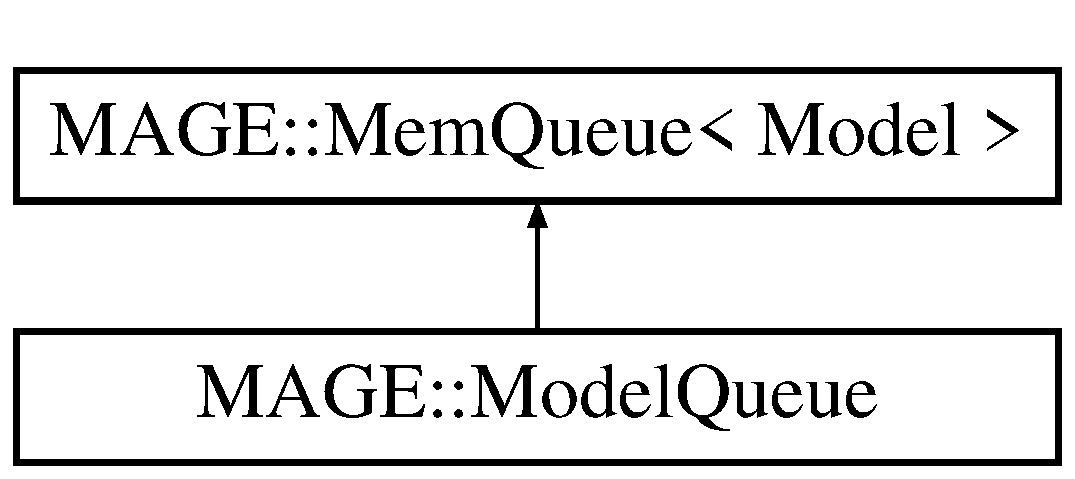
\includegraphics[height=2.000000cm]{class_m_a_g_e_1_1_model_queue}
\end{center}
\end{figure}
\subsection*{Public Member Functions}
\begin{DoxyCompactItemize}
\item 
\hypertarget{class_m_a_g_e_1_1_model_queue_a03f786d7dc7e7adad25216f8ec83752d}{{\bfseries Model\-Queue} (unsigned int queue\-Len)}\label{class_m_a_g_e_1_1_model_queue_a03f786d7dc7e7adad25216f8ec83752d}

\item 
\hypertarget{class_m_a_g_e_1_1_model_queue_ab1f2f92109e6fca56b51be0ead9b105d}{\hyperlink{class_m_a_g_e_1_1_model_queue_memory}{Model\-Queue\-Memory} $\ast$ {\bfseries get\-Model\-Queue\-Memory} (void)}\label{class_m_a_g_e_1_1_model_queue_ab1f2f92109e6fca56b51be0ead9b105d}

\item 
\hypertarget{class_m_a_g_e_1_1_model_queue_a566cc6d3e8f6e50a54da65f185592629}{void {\bfseries print\-Queue} (void)}\label{class_m_a_g_e_1_1_model_queue_a566cc6d3e8f6e50a54da65f185592629}

\item 
\hypertarget{class_m_a_g_e_1_1_model_queue_a6592defce9e72de3cfc266ae5e52e86d}{void {\bfseries generate} (\hyperlink{class_m_a_g_e_1_1_frame_queue}{Frame\-Queue} $\ast$frame\-Queue, unsigned int backup=n\-Of\-Backup)}\label{class_m_a_g_e_1_1_model_queue_a6592defce9e72de3cfc266ae5e52e86d}

\item 
\hypertarget{class_m_a_g_e_1_1_model_queue_a6c76b6ddff10f8caa21fc454325d3b77}{void {\bfseries optimize\-Parameters} (\hyperlink{class_m_a_g_e_1_1_engine}{M\-A\-G\-E\-::\-Engine} $\ast$engine, unsigned int backup=n\-Of\-Backup, unsigned int lookup=n\-Of\-Lookup)}\label{class_m_a_g_e_1_1_model_queue_a6c76b6ddff10f8caa21fc454325d3b77}

\end{DoxyCompactItemize}
\subsection*{Protected Attributes}
\begin{DoxyCompactItemize}
\item 
\hypertarget{class_m_a_g_e_1_1_model_queue_a15ff44566b9c488e977e2fd8cf11a85b}{\hyperlink{struct_m_a_g_e_1_1_frame}{Frame} $\ast$ {\bfseries frame}}\label{class_m_a_g_e_1_1_model_queue_a15ff44566b9c488e977e2fd8cf11a85b}

\item 
\hypertarget{class_m_a_g_e_1_1_model_queue_a8ce20b001dec594aeb232d0bab3adc6f}{unsigned int {\bfseries head}}\label{class_m_a_g_e_1_1_model_queue_a8ce20b001dec594aeb232d0bab3adc6f}

\item 
\hypertarget{class_m_a_g_e_1_1_model_queue_aac94662cccf3527e70879cc3f58c2ece}{\hyperlink{class_m_a_g_e_1_1_model_queue_memory}{Model\-Queue\-Memory} {\bfseries model\-Queue\-Memory}}\label{class_m_a_g_e_1_1_model_queue_aac94662cccf3527e70879cc3f58c2ece}

\end{DoxyCompactItemize}


The documentation for this class was generated from the following files\-:\begin{DoxyCompactItemize}
\item 
/\-Users/\-Maipn/\-Documents/my\-Libs/\-M\-A\-G\-E/magelib-\/2.\-00/src/\hyperlink{_model_queue_8h}{Model\-Queue.\-h}\item 
/\-Users/\-Maipn/\-Documents/my\-Libs/\-M\-A\-G\-E/magelib-\/2.\-00/src/\hyperlink{_model_queue_8cpp}{Model\-Queue.\-cpp}\end{DoxyCompactItemize}

\hypertarget{class_m_a_g_e_1_1_model_queue_memory}{\section{M\-A\-G\-E\-:\-:Model\-Queue\-Memory Class Reference}
\label{class_m_a_g_e_1_1_model_queue_memory}\index{M\-A\-G\-E\-::\-Model\-Queue\-Memory@{M\-A\-G\-E\-::\-Model\-Queue\-Memory}}
}
\subsection*{Public Attributes}
\begin{DoxyCompactItemize}
\item 
\hypertarget{class_m_a_g_e_1_1_model_queue_memory_a6831d4cdf1472693fc85f4d3c53ea7f4}{double $\ast$$\ast$$\ast$ {\bfseries mean}}\label{class_m_a_g_e_1_1_model_queue_memory_a6831d4cdf1472693fc85f4d3c53ea7f4}

\item 
\hypertarget{class_m_a_g_e_1_1_model_queue_memory_a636545600f4ee5360b7d9782c9042744}{double $\ast$$\ast$$\ast$ {\bfseries ivar}}\label{class_m_a_g_e_1_1_model_queue_memory_a636545600f4ee5360b7d9782c9042744}

\item 
\hypertarget{class_m_a_g_e_1_1_model_queue_memory_ad80de821c46d9cf83e0659cb3042bf3e}{double $\ast$$\ast$ {\bfseries gv\-\_\-mean}}\label{class_m_a_g_e_1_1_model_queue_memory_ad80de821c46d9cf83e0659cb3042bf3e}

\item 
\hypertarget{class_m_a_g_e_1_1_model_queue_memory_a1d4e17199ea97e1b4a11c7d20e7151f0}{double $\ast$$\ast$ {\bfseries gv\-\_\-vari}}\label{class_m_a_g_e_1_1_model_queue_memory_a1d4e17199ea97e1b4a11c7d20e7151f0}

\item 
\hypertarget{class_m_a_g_e_1_1_model_queue_memory_a3ef2b07a2bec7fac84e5adb6ac1ca249}{int $\ast$$\ast$ {\bfseries gv\-\_\-switch}}\label{class_m_a_g_e_1_1_model_queue_memory_a3ef2b07a2bec7fac84e5adb6ac1ca249}

\item 
\hypertarget{class_m_a_g_e_1_1_model_queue_memory_a9e55a05bc4a9545bfd7af6238843a6e9}{double $\ast$$\ast$ {\bfseries g}}\label{class_m_a_g_e_1_1_model_queue_memory_a9e55a05bc4a9545bfd7af6238843a6e9}

\item 
\hypertarget{class_m_a_g_e_1_1_model_queue_memory_ae7bad2f0e36ec2ca981f4516d2ee98eb}{double $\ast$$\ast$ {\bfseries wum}}\label{class_m_a_g_e_1_1_model_queue_memory_ae7bad2f0e36ec2ca981f4516d2ee98eb}

\item 
\hypertarget{class_m_a_g_e_1_1_model_queue_memory_ae4956587c224f47c013fbade1181716e}{double $\ast$$\ast$$\ast$ {\bfseries wuw}}\label{class_m_a_g_e_1_1_model_queue_memory_ae4956587c224f47c013fbade1181716e}

\item 
\hypertarget{class_m_a_g_e_1_1_model_queue_memory_aebc11b875893cb9f893042acda3654d0}{double $\ast$$\ast$$\ast$ {\bfseries par}}\label{class_m_a_g_e_1_1_model_queue_memory_aebc11b875893cb9f893042acda3654d0}

\item 
\hypertarget{class_m_a_g_e_1_1_model_queue_memory_a109bd7570f9690fcc3662381042e7b05}{int $\ast$ {\bfseries voiced\-\_\-unvoiced}}\label{class_m_a_g_e_1_1_model_queue_memory_a109bd7570f9690fcc3662381042e7b05}

\end{DoxyCompactItemize}


The documentation for this class was generated from the following files\-:\begin{DoxyCompactItemize}
\item 
/\-Users/\-Maipn/\-Documents/my\-Libs/\-M\-A\-G\-E/magelib-\/2.\-00/src/\hyperlink{_model_queue_8h}{Model\-Queue.\-h}\item 
/\-Users/\-Maipn/\-Documents/my\-Libs/\-M\-A\-G\-E/magelib-\/2.\-00/src/\hyperlink{_model_queue_8cpp}{Model\-Queue.\-cpp}\end{DoxyCompactItemize}

\hypertarget{struct_m_a_g_e_1_1_m_s_distribution}{\section{M\-A\-G\-E\-:\-:M\-S\-Distribution Struct Reference}
\label{struct_m_a_g_e_1_1_m_s_distribution}\index{M\-A\-G\-E\-::\-M\-S\-Distribution@{M\-A\-G\-E\-::\-M\-S\-Distribution}}
}
Inheritance diagram for M\-A\-G\-E\-:\-:M\-S\-Distribution\-:\begin{figure}[H]
\begin{center}
\leavevmode
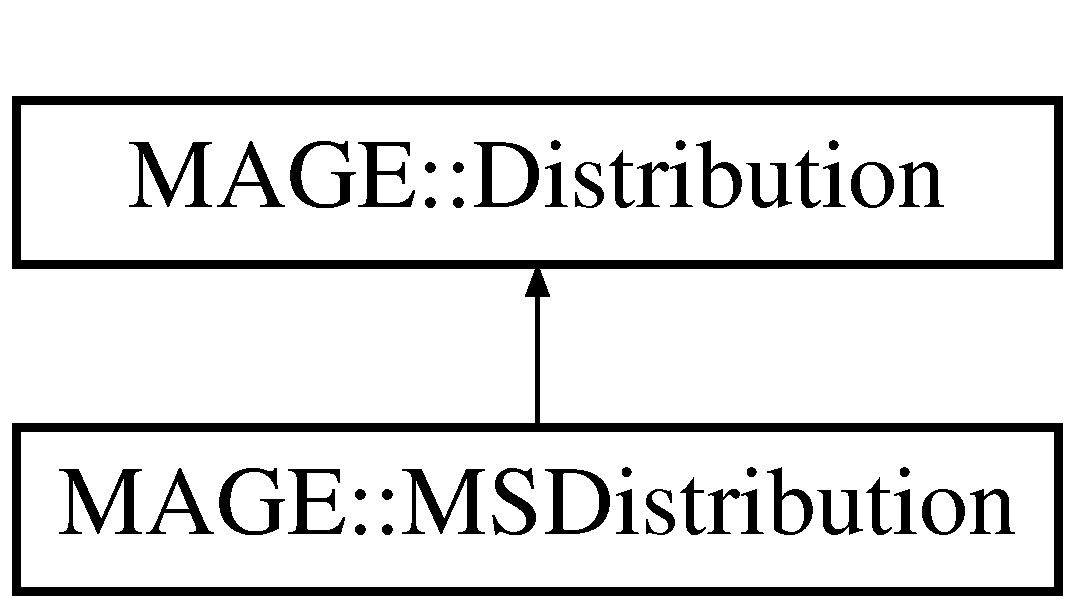
\includegraphics[height=2.000000cm]{struct_m_a_g_e_1_1_m_s_distribution}
\end{center}
\end{figure}
\subsection*{Public Attributes}
\begin{DoxyCompactItemize}
\item 
\hypertarget{struct_m_a_g_e_1_1_m_s_distribution_a0ed9157691205923f9555223b473387a}{double {\bfseries msd\-Flag}}\label{struct_m_a_g_e_1_1_m_s_distribution_a0ed9157691205923f9555223b473387a}

\end{DoxyCompactItemize}


The documentation for this struct was generated from the following file\-:\begin{DoxyCompactItemize}
\item 
/\-Users/\-Maipn/\-Documents/my\-Libs/\-M\-A\-G\-E/magelib-\/2.\-00/src/M\-S\-Distribution.\-h\end{DoxyCompactItemize}

\hypertarget{struct_m_a_g_e_1_1_state}{\section{M\-A\-G\-E\-:\-:State Struct Reference}
\label{struct_m_a_g_e_1_1_state}\index{M\-A\-G\-E\-::\-State@{M\-A\-G\-E\-::\-State}}
}


Definition of the H\-M\-Ms.  




{\ttfamily \#include $<$State.\-h$>$}

\subsection*{Public Attributes}
\begin{DoxyCompactItemize}
\item 
\hypertarget{struct_m_a_g_e_1_1_state_a374a7cb32876f8190f7ee541283f969a}{int \hyperlink{struct_m_a_g_e_1_1_state_a374a7cb32876f8190f7ee541283f969a}{duration}}\label{struct_m_a_g_e_1_1_state_a374a7cb32876f8190f7ee541283f969a}

\begin{DoxyCompactList}\small\item\em It contains the duration of every state of a given H\-M\-M. \end{DoxyCompactList}\item 
\hypertarget{struct_m_a_g_e_1_1_state_af71881812290585c3ea318251c0bb3f5}{bool \hyperlink{struct_m_a_g_e_1_1_state_af71881812290585c3ea318251c0bb3f5}{mgc\-\_\-gv\-\_\-switch}}\label{struct_m_a_g_e_1_1_state_af71881812290585c3ea318251c0bb3f5}

\begin{DoxyCompactList}\small\item\em It contains the global variance flag of the spectral stream for every state of a given H\-M\-M. \end{DoxyCompactList}\item 
\hypertarget{struct_m_a_g_e_1_1_state_a77240283e31e92076c73ecc0f9dbc34f}{bool \hyperlink{struct_m_a_g_e_1_1_state_a77240283e31e92076c73ecc0f9dbc34f}{lf0\-\_\-gv\-\_\-switch}}\label{struct_m_a_g_e_1_1_state_a77240283e31e92076c73ecc0f9dbc34f}

\begin{DoxyCompactList}\small\item\em It contains the global variance flag of the fundamental frequency stream for every state of a given H\-M\-M. \end{DoxyCompactList}\item 
\hypertarget{struct_m_a_g_e_1_1_state_a174dfed9ae24aff59d3f69d0733478e5}{bool \hyperlink{struct_m_a_g_e_1_1_state_a174dfed9ae24aff59d3f69d0733478e5}{lpf\-\_\-gv\-\_\-switch}}\label{struct_m_a_g_e_1_1_state_a174dfed9ae24aff59d3f69d0733478e5}

\begin{DoxyCompactList}\small\item\em It contains the global variance flag of the low-\/pass filtering stream for every state of a given H\-M\-M. \end{DoxyCompactList}\item 
\hypertarget{struct_m_a_g_e_1_1_state_a1a8511f007e662b79fc204e4cb3261a4}{\hyperlink{struct_m_a_g_e_1_1_distribution}{Distribution} \hyperlink{struct_m_a_g_e_1_1_state_a1a8511f007e662b79fc204e4cb3261a4}{mgc} \mbox{[}n\-Of\-Ders $\ast$n\-Of\-M\-G\-Cs\mbox{]}}\label{struct_m_a_g_e_1_1_state_a1a8511f007e662b79fc204e4cb3261a4}

\begin{DoxyCompactList}\small\item\em It contains the gaussian distribution (including static and dynamic features) of the spectral stream for every state of a given H\-M\-M. \end{DoxyCompactList}\item 
\hypertarget{struct_m_a_g_e_1_1_state_a5e97786bd0abad3f676aab2e4238bd58}{\hyperlink{struct_m_a_g_e_1_1_m_s_distribution}{M\-S\-Distribution} \hyperlink{struct_m_a_g_e_1_1_state_a5e97786bd0abad3f676aab2e4238bd58}{lf0} \mbox{[}n\-Of\-Ders $\ast$n\-Of\-L\-F0s\mbox{]}}\label{struct_m_a_g_e_1_1_state_a5e97786bd0abad3f676aab2e4238bd58}

\begin{DoxyCompactList}\small\item\em It contains the gaussian distribution (including static and dynamic features) of the fundamental frequency stream for every state of a given H\-M\-M. \end{DoxyCompactList}\item 
\hypertarget{struct_m_a_g_e_1_1_state_a6d3ea7b615c59e014d82ebf67ae2766d}{\hyperlink{struct_m_a_g_e_1_1_distribution}{Distribution} \hyperlink{struct_m_a_g_e_1_1_state_a6d3ea7b615c59e014d82ebf67ae2766d}{lpf} \mbox{[}n\-Of\-Ders $\ast$n\-Of\-L\-P\-Fs\mbox{]}}\label{struct_m_a_g_e_1_1_state_a6d3ea7b615c59e014d82ebf67ae2766d}

\begin{DoxyCompactList}\small\item\em It contains the gaussian distribution (including static and dynamic features) of the low-\/pass filtering stream for every state of a given H\-M\-M. \end{DoxyCompactList}\item 
\hypertarget{struct_m_a_g_e_1_1_state_a69a8e57098ea4126782a671d42485f82}{\hyperlink{struct_m_a_g_e_1_1_distribution}{Distribution} \hyperlink{struct_m_a_g_e_1_1_state_a69a8e57098ea4126782a671d42485f82}{gv\-\_\-mgc} \mbox{[}n\-Of\-Ders $\ast$n\-Of\-M\-G\-Cs\mbox{]}}\label{struct_m_a_g_e_1_1_state_a69a8e57098ea4126782a671d42485f82}

\begin{DoxyCompactList}\small\item\em It contains the gaussian distribution (including static and dynamic features) of the global variance of the spectral stream for every state of a given H\-M\-M. \end{DoxyCompactList}\item 
\hypertarget{struct_m_a_g_e_1_1_state_a3d3ecc2eaccfe03e5b30b2919eeb3df2}{\hyperlink{struct_m_a_g_e_1_1_distribution}{Distribution} \hyperlink{struct_m_a_g_e_1_1_state_a3d3ecc2eaccfe03e5b30b2919eeb3df2}{gv\-\_\-lf0} \mbox{[}n\-Of\-Ders $\ast$n\-Of\-L\-F0s\mbox{]}}\label{struct_m_a_g_e_1_1_state_a3d3ecc2eaccfe03e5b30b2919eeb3df2}

\begin{DoxyCompactList}\small\item\em It contains the gaussian distribution (including static and dynamic features) of the global variance of the fundamental frequency stream for every state of a given H\-M\-M. \end{DoxyCompactList}\item 
\hypertarget{struct_m_a_g_e_1_1_state_a849ff0368b589c4e298340450952a39b}{\hyperlink{struct_m_a_g_e_1_1_distribution}{Distribution} \hyperlink{struct_m_a_g_e_1_1_state_a849ff0368b589c4e298340450952a39b}{gv\-\_\-lpf} \mbox{[}n\-Of\-Ders $\ast$n\-Of\-L\-P\-Fs\mbox{]}}\label{struct_m_a_g_e_1_1_state_a849ff0368b589c4e298340450952a39b}

\begin{DoxyCompactList}\small\item\em It contains the gaussian distribution (including static and dynamic features) of the global variance of the low-\/pass filtering stream for every state of a given H\-M\-M. \end{DoxyCompactList}\end{DoxyCompactItemize}


\subsection{Detailed Description}
Definition of the H\-M\-Ms. 

This struct is used to define every state of the H\-M\-Ms used. Here it contains the duration and distributions used in every state of H\-M\-M.

\begin{DoxyAuthor}{Authors}
Maria Astrinaki, Alexis Moinet, Geoffrey Wilfart, Nicolas d'Alessandro, Thierry Dutoit
\end{DoxyAuthor}
\begin{DoxyVersion}{Version}
2.\-00 beta 
\end{DoxyVersion}
\begin{DoxyDate}{Date}
2011 -\/ 2012 
\end{DoxyDate}
\begin{DoxyCopyright}{Copyright}
Numediart Institute for New Media Art ( www.\-numediart.\-org ) \par
 Acapela Group ( www.\-acapela-\/group.\-com ) \par
 G\-N\-U Public License (see the licence in the file). 
\end{DoxyCopyright}


The documentation for this struct was generated from the following file\-:\begin{DoxyCompactItemize}
\item 
/\-Users/\-Maipn/\-Documents/my\-Libs/\-M\-A\-G\-E/magelib-\/2.\-00/src/State.\-h\end{DoxyCompactItemize}

\hypertarget{class_m_a_g_e_1_1_vocoder}{\section{M\-A\-G\-E\-:\-:Vocoder Class Reference}
\label{class_m_a_g_e_1_1_vocoder}\index{M\-A\-G\-E\-::\-Vocoder@{M\-A\-G\-E\-::\-Vocoder}}
}
\subsection*{Public Member Functions}
\begin{DoxyCompactItemize}
\item 
\hypertarget{class_m_a_g_e_1_1_vocoder_a0c949814cc5263ae226c23fb5ca7abf4}{{\bfseries Vocoder} (int am=(n\-Of\-M\-G\-Cs-\/1), double aalpha=default\-Alpha, int afprd=default\-Frame\-Rate, int aiprd=default\-Interp\-Frame\-Rate, int astage=default\-Gamma, int apd=default\-Pade\-Order, bool angain=false)}\label{class_m_a_g_e_1_1_vocoder_a0c949814cc5263ae226c23fb5ca7abf4}

\item 
\hypertarget{class_m_a_g_e_1_1_vocoder_aa6fcee8597d4c652f069e329ac115e42}{{\bfseries Vocoder} (const \hyperlink{class_m_a_g_e_1_1_vocoder}{Vocoder} \&orig)}\label{class_m_a_g_e_1_1_vocoder_aa6fcee8597d4c652f069e329ac115e42}

\item 
\hypertarget{class_m_a_g_e_1_1_vocoder_af5b257b55f3200e733a96af8b8e1013f}{double {\bfseries get\-Alpha} (void)}\label{class_m_a_g_e_1_1_vocoder_af5b257b55f3200e733a96af8b8e1013f}

\item 
\hypertarget{class_m_a_g_e_1_1_vocoder_a2e3e6b7d223c8e253901a30709b39100}{double {\bfseries get\-Pitch} (void)}\label{class_m_a_g_e_1_1_vocoder_a2e3e6b7d223c8e253901a30709b39100}

\item 
\hypertarget{class_m_a_g_e_1_1_vocoder_a76b9cc7b27f27760b8f6d4c2f14cd2ed}{double {\bfseries get\-Period} (void)}\label{class_m_a_g_e_1_1_vocoder_a76b9cc7b27f27760b8f6d4c2f14cd2ed}

\item 
\hypertarget{class_m_a_g_e_1_1_vocoder_a5f5bb1141cc727462434116b9dd24e42}{double {\bfseries get\-Volume} (void)}\label{class_m_a_g_e_1_1_vocoder_a5f5bb1141cc727462434116b9dd24e42}

\item 
\hypertarget{class_m_a_g_e_1_1_vocoder_a9d4b3e4f17d2a710eb29c18acfd2db09}{double {\bfseries get\-Pade\-Order} (void)}\label{class_m_a_g_e_1_1_vocoder_a9d4b3e4f17d2a710eb29c18acfd2db09}

\item 
\hypertarget{class_m_a_g_e_1_1_vocoder_ac0707389d3fcb19a1acc4e44ef5b2d94}{int {\bfseries get\-Action} (void)}\label{class_m_a_g_e_1_1_vocoder_ac0707389d3fcb19a1acc4e44ef5b2d94}

\item 
\hypertarget{class_m_a_g_e_1_1_vocoder_aa69d3116f7989880455766230d8af06c}{double {\bfseries get\-Gamma} (void)}\label{class_m_a_g_e_1_1_vocoder_aa69d3116f7989880455766230d8af06c}

\item 
\hypertarget{class_m_a_g_e_1_1_vocoder_a638ebd059ae6e38500f9bf0b62ffde79}{void {\bfseries set\-Alpha} (double aalpha)}\label{class_m_a_g_e_1_1_vocoder_a638ebd059ae6e38500f9bf0b62ffde79}

\item 
\hypertarget{class_m_a_g_e_1_1_vocoder_af7f2886e18a5ca7929a1031b86c1cf4b}{void {\bfseries set\-Gamma} (double agamma)}\label{class_m_a_g_e_1_1_vocoder_af7f2886e18a5ca7929a1031b86c1cf4b}

\item 
\hypertarget{class_m_a_g_e_1_1_vocoder_abe8aa23071fe0b6ba424a4f0105b3788}{void {\bfseries set\-Volume} (double avolume)}\label{class_m_a_g_e_1_1_vocoder_abe8aa23071fe0b6ba424a4f0105b3788}

\item 
\hypertarget{class_m_a_g_e_1_1_vocoder_a67cdc9e3f2f2561782944b6702fff7d1}{void {\bfseries set\-Pade\-Order} (double apd)}\label{class_m_a_g_e_1_1_vocoder_a67cdc9e3f2f2561782944b6702fff7d1}

\item 
\hypertarget{class_m_a_g_e_1_1_vocoder_a56823e2f6437744f5d2ceb2ec973b3f2}{void {\bfseries set\-Voiced} (bool force\-Voiced)}\label{class_m_a_g_e_1_1_vocoder_a56823e2f6437744f5d2ceb2ec973b3f2}

\item 
void \hyperlink{class_m_a_g_e_1_1_vocoder_ad0010897fe2f1b7ff08ff765b2c315b9}{set\-Pitch} (double pitch, int action, bool force\-Voiced=false)
\item 
void \hyperlink{class_m_a_g_e_1_1_vocoder_a090b14af5e7371412ebee3829808f2de}{push} (\hyperlink{struct_m_a_g_e_1_1_frame}{Frame} \&frame, bool ignore\-Voicing=false)
\item 
void \hyperlink{class_m_a_g_e_1_1_vocoder_a7fc53d29d82c2b6d8a4ff01650b9b4dd}{push} (\hyperlink{struct_m_a_g_e_1_1_frame}{Frame} $\ast$frame, bool ignore\-Voicing=false)
\item 
void \hyperlink{class_m_a_g_e_1_1_vocoder_aa219489f0b80f526dd97f19587b35239}{reset} (void)
\item 
bool \hyperlink{class_m_a_g_e_1_1_vocoder_af71ab9d9790777fb336354d1360b5c46}{ready} (void)
\item 
double \hyperlink{class_m_a_g_e_1_1_vocoder_a1ce94efa74a2b8f2391ddaf9443e60d7}{pop} (void)
\item 
\hypertarget{class_m_a_g_e_1_1_vocoder_a6082303317d5ce9424fc880a0e5b76c3}{bool {\bfseries is\-Voiced} (void)}\label{class_m_a_g_e_1_1_vocoder_a6082303317d5ce9424fc880a0e5b76c3}

\end{DoxyCompactItemize}
\subsection*{Protected Attributes}
\begin{DoxyCompactItemize}
\item 
\hypertarget{class_m_a_g_e_1_1_vocoder_a407749e074c4e722099af615da63684f}{double {\bfseries alpha}}\label{class_m_a_g_e_1_1_vocoder_a407749e074c4e722099af615da63684f}

\item 
\hypertarget{class_m_a_g_e_1_1_vocoder_a8fdaf7429b1457c2ec70cbc4080ca7a9}{double {\bfseries gamma}}\label{class_m_a_g_e_1_1_vocoder_a8fdaf7429b1457c2ec70cbc4080ca7a9}

\item 
\hypertarget{class_m_a_g_e_1_1_vocoder_a9433e206e040793167b2bb12dff07430}{double {\bfseries f0}}\label{class_m_a_g_e_1_1_vocoder_a9433e206e040793167b2bb12dff07430}

\item 
\hypertarget{class_m_a_g_e_1_1_vocoder_a2989b96b629bc07f2a1b09f01b6fa1fd}{double {\bfseries t0}}\label{class_m_a_g_e_1_1_vocoder_a2989b96b629bc07f2a1b09f01b6fa1fd}

\item 
\hypertarget{class_m_a_g_e_1_1_vocoder_a5ad040b2ba593e638a29c015c8a8212a}{bool {\bfseries voiced}}\label{class_m_a_g_e_1_1_vocoder_a5ad040b2ba593e638a29c015c8a8212a}

\item 
\hypertarget{class_m_a_g_e_1_1_vocoder_a5c141fafcec68091378466e7bdc5b1d7}{int {\bfseries action}}\label{class_m_a_g_e_1_1_vocoder_a5c141fafcec68091378466e7bdc5b1d7}

\end{DoxyCompactItemize}


\subsection{Member Function Documentation}
\hypertarget{class_m_a_g_e_1_1_vocoder_a1ce94efa74a2b8f2391ddaf9443e60d7}{\index{M\-A\-G\-E\-::\-Vocoder@{M\-A\-G\-E\-::\-Vocoder}!pop@{pop}}
\index{pop@{pop}!MAGE::Vocoder@{M\-A\-G\-E\-::\-Vocoder}}
\subsubsection[{pop}]{\setlength{\rightskip}{0pt plus 5cm}double M\-A\-G\-E\-::\-Vocoder\-::pop (
\begin{DoxyParamCaption}
\item[{void}]{}
\end{DoxyParamCaption}
)}}\label{class_m_a_g_e_1_1_vocoder_a1ce94efa74a2b8f2391ddaf9443e60d7}
\begin{DoxyReturn}{Returns}
one sample from the vocoder given current mgc and lf0 
\end{DoxyReturn}
\hypertarget{class_m_a_g_e_1_1_vocoder_a090b14af5e7371412ebee3829808f2de}{\index{M\-A\-G\-E\-::\-Vocoder@{M\-A\-G\-E\-::\-Vocoder}!push@{push}}
\index{push@{push}!MAGE::Vocoder@{M\-A\-G\-E\-::\-Vocoder}}
\subsubsection[{push}]{\setlength{\rightskip}{0pt plus 5cm}void M\-A\-G\-E\-::\-Vocoder\-::push (
\begin{DoxyParamCaption}
\item[{{\bf Frame} \&}]{frame, }
\item[{bool}]{ignore\-Voicing = {\ttfamily false}}
\end{DoxyParamCaption}
)}}\label{class_m_a_g_e_1_1_vocoder_a090b14af5e7371412ebee3829808f2de}

\begin{DoxyParams}{Parameters}
{\em frame} & an instance of class \hyperlink{struct_m_a_g_e_1_1_frame}{Frame} \\
\hline
{\em ignore\-Voicing} & if true, ignore frame.\-voiced information and use latest known information \\
\hline
\end{DoxyParams}
\hypertarget{class_m_a_g_e_1_1_vocoder_a7fc53d29d82c2b6d8a4ff01650b9b4dd}{\index{M\-A\-G\-E\-::\-Vocoder@{M\-A\-G\-E\-::\-Vocoder}!push@{push}}
\index{push@{push}!MAGE::Vocoder@{M\-A\-G\-E\-::\-Vocoder}}
\subsubsection[{push}]{\setlength{\rightskip}{0pt plus 5cm}void M\-A\-G\-E\-::\-Vocoder\-::push (
\begin{DoxyParamCaption}
\item[{{\bf Frame} $\ast$}]{frame, }
\item[{bool}]{ignore\-Voicing = {\ttfamily false}}
\end{DoxyParamCaption}
)}}\label{class_m_a_g_e_1_1_vocoder_a7fc53d29d82c2b6d8a4ff01650b9b4dd}

\begin{DoxyParams}{Parameters}
{\em frame} & a pointer to an instance of class \hyperlink{struct_m_a_g_e_1_1_frame}{Frame} \\
\hline
{\em ignore\-Voicing} & if true, ignore frame-\/$>$voiced information and use latest known information \\
\hline
\end{DoxyParams}
\hypertarget{class_m_a_g_e_1_1_vocoder_af71ab9d9790777fb336354d1360b5c46}{\index{M\-A\-G\-E\-::\-Vocoder@{M\-A\-G\-E\-::\-Vocoder}!ready@{ready}}
\index{ready@{ready}!MAGE::Vocoder@{M\-A\-G\-E\-::\-Vocoder}}
\subsubsection[{ready}]{\setlength{\rightskip}{0pt plus 5cm}bool M\-A\-G\-E\-::\-Vocoder\-::ready (
\begin{DoxyParamCaption}
\item[{void}]{}
\end{DoxyParamCaption}
)}}\label{class_m_a_g_e_1_1_vocoder_af71ab9d9790777fb336354d1360b5c46}
\begin{DoxyReturn}{Returns}
true if at least one frame has been pushed, false otherwise 
\end{DoxyReturn}
\hypertarget{class_m_a_g_e_1_1_vocoder_aa219489f0b80f526dd97f19587b35239}{\index{M\-A\-G\-E\-::\-Vocoder@{M\-A\-G\-E\-::\-Vocoder}!reset@{reset}}
\index{reset@{reset}!MAGE::Vocoder@{M\-A\-G\-E\-::\-Vocoder}}
\subsubsection[{reset}]{\setlength{\rightskip}{0pt plus 5cm}void M\-A\-G\-E\-::\-Vocoder\-::reset (
\begin{DoxyParamCaption}
\item[{void}]{}
\end{DoxyParamCaption}
)}}\label{class_m_a_g_e_1_1_vocoder_aa219489f0b80f526dd97f19587b35239}
Set the internal members of \hyperlink{class_m_a_g_e_1_1_vocoder}{Vocoder} to the contructor values. To be used in case the vocoder becomes irremediably unstable \hypertarget{class_m_a_g_e_1_1_vocoder_ad0010897fe2f1b7ff08ff765b2c315b9}{\index{M\-A\-G\-E\-::\-Vocoder@{M\-A\-G\-E\-::\-Vocoder}!set\-Pitch@{set\-Pitch}}
\index{set\-Pitch@{set\-Pitch}!MAGE::Vocoder@{M\-A\-G\-E\-::\-Vocoder}}
\subsubsection[{set\-Pitch}]{\setlength{\rightskip}{0pt plus 5cm}void M\-A\-G\-E\-::\-Vocoder\-::set\-Pitch (
\begin{DoxyParamCaption}
\item[{double}]{pitch, }
\item[{int}]{action, }
\item[{bool}]{force\-Voiced = {\ttfamily false}}
\end{DoxyParamCaption}
)}}\label{class_m_a_g_e_1_1_vocoder_ad0010897fe2f1b7ff08ff765b2c315b9}
This function forces the value of the pitch used by the vocoder instead of the one in frame.\-f0. Note that this will get overwritten at the next push( frame ). Therefore it is needed to call \hyperlink{class_m_a_g_e_1_1_vocoder_ad0010897fe2f1b7ff08ff765b2c315b9}{set\-Pitch()}after every \hyperlink{class_m_a_g_e_1_1_vocoder_a090b14af5e7371412ebee3829808f2de}{push()}. Another solution is to call push( frame,true )which explicitely tells push to ignore voicing information.


\begin{DoxyParams}{Parameters}
{\em pitch} & pitch value in Hz \\
\hline
{\em force\-Voiced} & in case the current frame is unvoiced, you can force it to become voiced with the given pitch otherwise it would ignore the pitch set until next frame \\
\hline
\end{DoxyParams}


The documentation for this class was generated from the following files\-:\begin{DoxyCompactItemize}
\item 
/\-Users/\-Maipn/\-Documents/my\-Libs/\-M\-A\-G\-E/magelib-\/2.\-00/src/\hyperlink{_vocoder_8h}{Vocoder.\-h}\item 
/\-Users/\-Maipn/\-Documents/my\-Libs/\-M\-A\-G\-E/magelib-\/2.\-00/src/\hyperlink{_vocoder_8cpp}{Vocoder.\-cpp}\end{DoxyCompactItemize}

\chapter{File Documentation}
\hypertarget{_constants_8h}{\section{/\-Users/\-Maipn/\-Documents/my\-Libs/\-M\-A\-G\-E/magelib-\/2.00/src/\-Constants.h File Reference}
\label{_constants_8h}\index{/\-Users/\-Maipn/\-Documents/my\-Libs/\-M\-A\-G\-E/magelib-\/2.\-00/src/\-Constants.\-h@{/\-Users/\-Maipn/\-Documents/my\-Libs/\-M\-A\-G\-E/magelib-\/2.\-00/src/\-Constants.\-h}}
}
\subsection*{Variables}
\begin{DoxyCompactItemize}
\item 
\hypertarget{namespace_m_a_g_e_a51faac58888055285b9bea607226e673}{const unsigned int {\bfseries M\-A\-G\-E\-::n\-Of\-Ders} = 3}\label{namespace_m_a_g_e_a51faac58888055285b9bea607226e673}

\item 
\hypertarget{namespace_m_a_g_e_a052a7a46d76c95ee2a25c90c7dd172e1}{const unsigned int {\bfseries M\-A\-G\-E\-::n\-Of\-M\-G\-Cs} = 35}\label{namespace_m_a_g_e_a052a7a46d76c95ee2a25c90c7dd172e1}

\item 
\hypertarget{namespace_m_a_g_e_a75c4bcc4f8ec1af6be6b1b6af89d9af5}{const unsigned int {\bfseries M\-A\-G\-E\-::n\-Of\-L\-F0s} = 1}\label{namespace_m_a_g_e_a75c4bcc4f8ec1af6be6b1b6af89d9af5}

\item 
\hypertarget{namespace_m_a_g_e_a975bdb463a4319fa817dab74f3e5f919}{const unsigned int {\bfseries M\-A\-G\-E\-::n\-Of\-L\-P\-Fs} = 31}\label{namespace_m_a_g_e_a975bdb463a4319fa817dab74f3e5f919}

\item 
\hypertarget{namespace_m_a_g_e_a1601229625b4bb57090b276109638323}{const unsigned int {\bfseries M\-A\-G\-E\-::n\-Of\-States} = 5}\label{namespace_m_a_g_e_a1601229625b4bb57090b276109638323}

\item 
\hypertarget{namespace_m_a_g_e_a5cab4d4a31028ec7d684077a782508d5}{const unsigned int {\bfseries M\-A\-G\-E\-::n\-Of\-Streams} = 3}\label{namespace_m_a_g_e_a5cab4d4a31028ec7d684077a782508d5}

\item 
\hypertarget{namespace_m_a_g_e_aa05ddefa96a94e42421eebea57141c6c}{const unsigned int {\bfseries M\-A\-G\-E\-::n\-Of\-Lookup} = 1}\label{namespace_m_a_g_e_aa05ddefa96a94e42421eebea57141c6c}

\item 
\hypertarget{namespace_m_a_g_e_afeaa9334040c794c816b9d0dec4045c2}{const unsigned int {\bfseries M\-A\-G\-E\-::n\-Of\-Backup} = 2}\label{namespace_m_a_g_e_afeaa9334040c794c816b9d0dec4045c2}

\item 
\hypertarget{namespace_m_a_g_e_ab940fabf4b498878ac92f4bacf7a0dbc}{const int {\bfseries M\-A\-G\-E\-::max\-Window\-Width} = 50}\label{namespace_m_a_g_e_ab940fabf4b498878ac92f4bacf7a0dbc}

\item 
\hypertarget{namespace_m_a_g_e_ad4a58c876332c54ba8b05b80cf82d00d}{const int {\bfseries M\-A\-G\-E\-::max\-Num\-Of\-Frames} = 512}\label{namespace_m_a_g_e_ad4a58c876332c54ba8b05b80cf82d00d}

\item 
\hypertarget{namespace_m_a_g_e_a0f62945e9c0cf6ecc76a2b181497556c}{const int {\bfseries M\-A\-G\-E\-::max\-Label\-Queue\-Len} = 512}\label{namespace_m_a_g_e_a0f62945e9c0cf6ecc76a2b181497556c}

\item 
\hypertarget{namespace_m_a_g_e_a1039e56e904d9d67f056bb9e4277b0b5}{const int {\bfseries M\-A\-G\-E\-::max\-Frame\-Queue\-Len} = 200}\label{namespace_m_a_g_e_a1039e56e904d9d67f056bb9e4277b0b5}

\item 
\hypertarget{namespace_m_a_g_e_adef8aabcbe7798af46e9763d5a6e4628}{const int {\bfseries M\-A\-G\-E\-::max\-Model\-Queue\-Len} = n\-Of\-Lookup + n\-Of\-Backup + 2}\label{namespace_m_a_g_e_adef8aabcbe7798af46e9763d5a6e4628}

\item 
\hypertarget{namespace_m_a_g_e_ab2bf5e717d3e772cdef44df8bd6557ad}{const double {\bfseries M\-A\-G\-E\-::default\-Alpha} = 0.\-55}\label{namespace_m_a_g_e_ab2bf5e717d3e772cdef44df8bd6557ad}

\item 
\hypertarget{namespace_m_a_g_e_a1f02bdc93d4ba82b88cd94ea5748059b}{const int {\bfseries M\-A\-G\-E\-::default\-Frame\-Rate} = 240}\label{namespace_m_a_g_e_a1f02bdc93d4ba82b88cd94ea5748059b}

\item 
\hypertarget{namespace_m_a_g_e_adbbdf48e539c84536079ea02ae1cb1d3}{const int {\bfseries M\-A\-G\-E\-::default\-Interp\-Frame\-Rate} = 1}\label{namespace_m_a_g_e_adbbdf48e539c84536079ea02ae1cb1d3}

\item 
\hypertarget{namespace_m_a_g_e_aaf66bc71efbd694a01ccf3121c3cc610}{const int {\bfseries M\-A\-G\-E\-::default\-Sampling\-Rate} = 48000}\label{namespace_m_a_g_e_aaf66bc71efbd694a01ccf3121c3cc610}

\item 
\hypertarget{namespace_m_a_g_e_a5f40bad0e2700f9d7eec355420209cb4}{const int {\bfseries M\-A\-G\-E\-::default\-Pade\-Order} = 5}\label{namespace_m_a_g_e_a5f40bad0e2700f9d7eec355420209cb4}

\item 
\hypertarget{namespace_m_a_g_e_a9af0a3b9dc76d8b2e39f10fc8cc10ec7}{const int {\bfseries M\-A\-G\-E\-::default\-Gamma} = 0}\label{namespace_m_a_g_e_a9af0a3b9dc76d8b2e39f10fc8cc10ec7}

\item 
\hypertarget{namespace_m_a_g_e_a05a3181ab06fffff791f99bf9df6dcee}{const int {\bfseries M\-A\-G\-E\-::default\-Volume} = 1}\label{namespace_m_a_g_e_a05a3181ab06fffff791f99bf9df6dcee}

\item 
\hypertarget{namespace_m_a_g_e_afe3d6b516bf2ddd0cce309b1b35effc7}{const int {\bfseries M\-A\-G\-E\-::mgc\-Stream\-Index} = 0}\label{namespace_m_a_g_e_afe3d6b516bf2ddd0cce309b1b35effc7}

\item 
\hypertarget{namespace_m_a_g_e_ae1590c9e012c9d9c614e0e17b71fead7}{const int {\bfseries M\-A\-G\-E\-::lf0\-Stream\-Index} = 1}\label{namespace_m_a_g_e_ae1590c9e012c9d9c614e0e17b71fead7}

\item 
\hypertarget{namespace_m_a_g_e_a862dc97415a1e8ab8959240d0c38567d}{const int {\bfseries M\-A\-G\-E\-::lpf\-Stream\-Index} = 2}\label{namespace_m_a_g_e_a862dc97415a1e8ab8959240d0c38567d}

\item 
\hypertarget{namespace_m_a_g_e_a94dc1d2aee01ea03c5616ab896f023d3}{const int {\bfseries M\-A\-G\-E\-::dur\-Stream\-Index} = 3}\label{namespace_m_a_g_e_a94dc1d2aee01ea03c5616ab896f023d3}

\item 
\hypertarget{namespace_m_a_g_e_ae448024a2434ab426b6eb2864ca4d6a0}{const int {\bfseries M\-A\-G\-E\-::mgc\-Len} = n\-Of\-Ders $\ast$ n\-Of\-M\-G\-Cs}\label{namespace_m_a_g_e_ae448024a2434ab426b6eb2864ca4d6a0}

\item 
\hypertarget{namespace_m_a_g_e_aa93924432bf812ff05dab21f1ffbaf32}{const int {\bfseries M\-A\-G\-E\-::lf0\-Len} = n\-Of\-Ders $\ast$ n\-Of\-L\-F0s}\label{namespace_m_a_g_e_aa93924432bf812ff05dab21f1ffbaf32}

\item 
\hypertarget{namespace_m_a_g_e_ac44f5816340536d7c3350dc9ff56e559}{const int {\bfseries M\-A\-G\-E\-::lpf\-Len} = n\-Of\-Ders $\ast$ n\-Of\-L\-P\-Fs}\label{namespace_m_a_g_e_ac44f5816340536d7c3350dc9ff56e559}

\item 
\hypertarget{namespace_m_a_g_e_adff3e7a6c9e0bd6c78982e29f946b131}{const int {\bfseries M\-A\-G\-E\-::noaction} = -\/1}\label{namespace_m_a_g_e_adff3e7a6c9e0bd6c78982e29f946b131}

\item 
\hypertarget{namespace_m_a_g_e_aff9d55e1160243060a2eff3f3ee0b1d6}{const int {\bfseries M\-A\-G\-E\-::overwrite} = 0}\label{namespace_m_a_g_e_aff9d55e1160243060a2eff3f3ee0b1d6}

\item 
\hypertarget{namespace_m_a_g_e_a8a38b5e1998068ddd8c6037925561945}{const int {\bfseries M\-A\-G\-E\-::shift} = 1}\label{namespace_m_a_g_e_a8a38b5e1998068ddd8c6037925561945}

\item 
\hypertarget{namespace_m_a_g_e_a6f86b724735cda5a8243392b24cdb3ef}{const int {\bfseries M\-A\-G\-E\-::scale} = 2}\label{namespace_m_a_g_e_a6f86b724735cda5a8243392b24cdb3ef}

\item 
\hypertarget{namespace_m_a_g_e_a6cac226dc53fdcfe78b5478568d15ba8}{const int {\bfseries M\-A\-G\-E\-::synthetic} = 3}\label{namespace_m_a_g_e_a6cac226dc53fdcfe78b5478568d15ba8}

\item 
\hypertarget{namespace_m_a_g_e_acf59391d7f0ea3cbe5cea815bdc8a92f}{const int {\bfseries M\-A\-G\-E\-::max\-Num\-Of\-Arguments} = 100}\label{namespace_m_a_g_e_acf59391d7f0ea3cbe5cea815bdc8a92f}

\item 
\hypertarget{namespace_m_a_g_e_aecaa791f74be49fa20a279fc68eeadff}{const int {\bfseries M\-A\-G\-E\-::max\-Str\-Len} = 1024}\label{namespace_m_a_g_e_aecaa791f74be49fa20a279fc68eeadff}

\item 
\hypertarget{namespace_m_a_g_e_a0b2bdf6bd33e8418547f3d520e3778bc}{const double {\bfseries M\-A\-G\-E\-::default\-Interpolation\-Weight} = 1}\label{namespace_m_a_g_e_a0b2bdf6bd33e8418547f3d520e3778bc}

\end{DoxyCompactItemize}


\subsection{Detailed Description}
\begin{DoxyAuthor}{Author}
Maria Astrinaki, Alexis Moinet, Geoffrey Wilfart, Nicolas d'Alessandro, Thierry Dutoit 
\end{DoxyAuthor}

\hypertarget{_frame_8h}{\section{/\-Users/\-Maipn/\-Documents/my\-Libs/\-M\-A\-G\-E/magelib-\/2.00/src/\-Frame.h File Reference}
\label{_frame_8h}\index{/\-Users/\-Maipn/\-Documents/my\-Libs/\-M\-A\-G\-E/magelib-\/2.\-00/src/\-Frame.\-h@{/\-Users/\-Maipn/\-Documents/my\-Libs/\-M\-A\-G\-E/magelib-\/2.\-00/src/\-Frame.\-h}}
}


Synthesis frame class.  


{\ttfamily \#include \char`\"{}Constants.\-h\char`\"{}}\\*
\subsection*{Classes}
\begin{DoxyCompactItemize}
\item 
struct \hyperlink{struct_m_a_g_e_1_1_frame}{M\-A\-G\-E\-::\-Frame}
\end{DoxyCompactItemize}


\subsection{Detailed Description}
Synthesis frame class. \begin{DoxyAuthor}{Author}
Maria Astrinaki, Alexis Moinet, Geoffrey Wilfart, Nicolas d'Alessandro, Thierry Dutoit 
\end{DoxyAuthor}

\hypertarget{_frame_queue_8cpp}{\section{/\-Users/\-Maipn/\-Documents/my\-Libs/\-M\-A\-G\-E/magelib-\/2.00/src/\-Frame\-Queue.cpp File Reference}
\label{_frame_queue_8cpp}\index{/\-Users/\-Maipn/\-Documents/my\-Libs/\-M\-A\-G\-E/magelib-\/2.\-00/src/\-Frame\-Queue.\-cpp@{/\-Users/\-Maipn/\-Documents/my\-Libs/\-M\-A\-G\-E/magelib-\/2.\-00/src/\-Frame\-Queue.\-cpp}}
}


Frame ringbuffer\-: used to exchange speech parameters with the synthesis thread.  


{\ttfamily \#include \char`\"{}Frame\-Queue.\-h\char`\"{}}\\*


\subsection{Detailed Description}
Frame ringbuffer\-: used to exchange speech parameters with the synthesis thread. \begin{DoxyAuthor}{Author}
Maria Astrinaki, Alexis Moinet, Geoffrey Wilfart, Nicolas d'Alessandro, Thierry Dutoit 
\end{DoxyAuthor}

\hypertarget{_frame_queue_8h}{\section{/\-Users/\-Maipn/\-Documents/my\-Libs/\-M\-A\-G\-E/magelib-\/2.00/src/\-Frame\-Queue.h File Reference}
\label{_frame_queue_8h}\index{/\-Users/\-Maipn/\-Documents/my\-Libs/\-M\-A\-G\-E/magelib-\/2.\-00/src/\-Frame\-Queue.\-h@{/\-Users/\-Maipn/\-Documents/my\-Libs/\-M\-A\-G\-E/magelib-\/2.\-00/src/\-Frame\-Queue.\-h}}
}


Frame ringbuffer\-: used to exchange speech parameters with the synthesis thread.  


{\ttfamily \#include \char`\"{}Mem\-Queue.\-h\char`\"{}}\\*
{\ttfamily \#include \char`\"{}Frame.\-h\char`\"{}}\\*
\subsection*{Classes}
\begin{DoxyCompactItemize}
\item 
class \hyperlink{class_m_a_g_e_1_1_frame_queue}{M\-A\-G\-E\-::\-Frame\-Queue}
\end{DoxyCompactItemize}


\subsection{Detailed Description}
Frame ringbuffer\-: used to exchange speech parameters with the synthesis thread. \begin{DoxyAuthor}{Author}
Maria Astrinaki, Alexis Moinet, Geoffrey Wilfart, Nicolas d'Alessandro, Thierry Dutoit 
\end{DoxyAuthor}

\hypertarget{hts_8cpp}{\section{/\-Users/\-Maipn/\-Documents/my\-Libs/\-M\-A\-G\-E/magelib-\/2.00/src/hts.cpp File Reference}
\label{hts_8cpp}\index{/\-Users/\-Maipn/\-Documents/my\-Libs/\-M\-A\-G\-E/magelib-\/2.\-00/src/hts.\-cpp@{/\-Users/\-Maipn/\-Documents/my\-Libs/\-M\-A\-G\-E/magelib-\/2.\-00/src/hts.\-cpp}}
}
{\ttfamily \#include \char`\"{}hts.\-h\char`\"{}}\\*
\subsection*{Functions}
\begin{DoxyCompactItemize}
\item 
\hypertarget{hts_8cpp_a40185ea52d16cecaafae70740e90af29}{void {\bfseries Usage} (void)}\label{hts_8cpp_a40185ea52d16cecaafae70740e90af29}

\item 
\hypertarget{hts_8cpp_ade080b2b3a230abbc162dbc840fe7df9}{void {\bfseries Error} (const int error, char $\ast$message,...)}\label{hts_8cpp_ade080b2b3a230abbc162dbc840fe7df9}

\item 
\hypertarget{hts_8cpp_a134f211ab996b0a1a00909eacec6a1a2}{int {\bfseries Get\-Num\-Interp} (int argc, char $\ast$$\ast$argv\-\_\-search)}\label{hts_8cpp_a134f211ab996b0a1a00909eacec6a1a2}

\item 
\hypertarget{hts_8cpp_ad96dba606b0178a13fc3211e8475c244}{bool {\bfseries isdigit\-\_\-string} (char $\ast$str)}\label{hts_8cpp_ad96dba606b0178a13fc3211e8475c244}

\item 
\hypertarget{hts_8cpp_a2502432c0d6cb36622bc5619dc35f37d}{double {\bfseries m\-H\-T\-S\-\_\-set\-\_\-duration} (int $\ast$duration, double $\ast$mean, double $\ast$vari, int size, double frame\-\_\-length)}\label{hts_8cpp_a2502432c0d6cb36622bc5619dc35f37d}

\item 
\hypertarget{hts_8cpp_a5f7fbda6fa2e87eaadd4024e5066eb1f}{double {\bfseries H\-T\-S\-\_\-finv} (const double x)}\label{hts_8cpp_a5f7fbda6fa2e87eaadd4024e5066eb1f}

\item 
\hypertarget{hts_8cpp_a8c1275605ff331b268d6387d4fd39dd9}{void {\bfseries H\-T\-S\-\_\-\-P\-Stream\-\_\-mlpg} (H\-T\-S\-\_\-\-P\-Stream $\ast$pst)}\label{hts_8cpp_a8c1275605ff331b268d6387d4fd39dd9}

\item 
\hypertarget{hts_8cpp_a164912f376f89a9c5d08669ad6e8ccb5}{void {\bfseries H\-T\-S\-\_\-\-P\-Stream\-\_\-calc\-\_\-wuw\-\_\-and\-\_\-wum} (H\-T\-S\-\_\-\-P\-Stream $\ast$pst, const int m)}\label{hts_8cpp_a164912f376f89a9c5d08669ad6e8ccb5}

\item 
\hypertarget{hts_8cpp_a870b4fa1b40ad11c8031a0dd5d47e61c}{void {\bfseries H\-T\-S\-\_\-\-P\-Stream\-\_\-ldl\-\_\-factorization} (H\-T\-S\-\_\-\-P\-Stream $\ast$pst)}\label{hts_8cpp_a870b4fa1b40ad11c8031a0dd5d47e61c}

\item 
\hypertarget{hts_8cpp_ae407a56aad8ff102e20cfbe08cbdf97b}{void {\bfseries H\-T\-S\-\_\-\-P\-Stream\-\_\-forward\-\_\-substitution} (H\-T\-S\-\_\-\-P\-Stream $\ast$pst)}\label{hts_8cpp_ae407a56aad8ff102e20cfbe08cbdf97b}

\item 
\hypertarget{hts_8cpp_ac49a7bc2eab2cbdec93a2e98e861880d}{void {\bfseries H\-T\-S\-\_\-\-P\-Stream\-\_\-backward\-\_\-substitution} (H\-T\-S\-\_\-\-P\-Stream $\ast$pst, const int m)}\label{hts_8cpp_ac49a7bc2eab2cbdec93a2e98e861880d}

\item 
\hypertarget{hts_8cpp_ad1e0140e378e294f736da44e17229a17}{void {\bfseries H\-T\-S\-\_\-\-P\-Stream\-\_\-gv\-\_\-parmgen} (H\-T\-S\-\_\-\-P\-Stream $\ast$pst, const int m)}\label{hts_8cpp_ad1e0140e378e294f736da44e17229a17}

\item 
\hypertarget{hts_8cpp_a153db6ffa6ddb40290297ec974df09a0}{void {\bfseries H\-T\-S\-\_\-\-P\-Stream\-\_\-conv\-\_\-gv} (H\-T\-S\-\_\-\-P\-Stream $\ast$pst, const int m)}\label{hts_8cpp_a153db6ffa6ddb40290297ec974df09a0}

\item 
\hypertarget{hts_8cpp_ab6f03b58c851c2a9cb99c7db11426c88}{double {\bfseries H\-T\-S\-\_\-\-P\-Stream\-\_\-calc\-\_\-derivative} (H\-T\-S\-\_\-\-P\-Stream $\ast$pst, const int m)}\label{hts_8cpp_ab6f03b58c851c2a9cb99c7db11426c88}

\item 
\hypertarget{hts_8cpp_a0454f4485d31e93f6cd02a3035f45daf}{void {\bfseries H\-T\-S\-\_\-\-P\-Stream\-\_\-calc\-\_\-gv} (H\-T\-S\-\_\-\-P\-Stream $\ast$pst, const int m, double $\ast$mean, double $\ast$vari)}\label{hts_8cpp_a0454f4485d31e93f6cd02a3035f45daf}

\end{DoxyCompactItemize}


\subsection{Detailed Description}
\begin{DoxyAuthor}{Author}
Maria Astrinaki, Alexis Moinet, Geoffrey Wilfart, Nicolas d'Alessandro, Thierry Dutoit 
\end{DoxyAuthor}

\hypertarget{hts_8h}{\section{/\-Users/\-Maipn/\-Documents/my\-Libs/\-M\-A\-G\-E/magelib-\/2.00/src/hts.h File Reference}
\label{hts_8h}\index{/\-Users/\-Maipn/\-Documents/my\-Libs/\-M\-A\-G\-E/magelib-\/2.\-00/src/hts.\-h@{/\-Users/\-Maipn/\-Documents/my\-Libs/\-M\-A\-G\-E/magelib-\/2.\-00/src/hts.\-h}}
}
{\ttfamily \#include \char`\"{}Math\-Functions.\-h\char`\"{}}\\*
{\ttfamily \#include \char`\"{}H\-T\-S\-\_\-engine.\-h\char`\"{}}\\*
{\ttfamily \#include \char`\"{}H\-T\-S\-\_\-hidden.\-h\char`\"{}}\\*
{\ttfamily \#include $<$string$>$}\\*
{\ttfamily \#include $<$stdarg.\-h$>$}\\*
{\ttfamily \#include $<$cstdlib$>$}\\*
\subsection*{Classes}
\begin{DoxyCompactItemize}
\item 
class \hyperlink{class_m_a_g_e_1_1_engine}{M\-A\-G\-E\-::\-Engine}
\end{DoxyCompactItemize}
\subsection*{Functions}
\begin{DoxyCompactItemize}
\item 
\hypertarget{hts_8h_a40185ea52d16cecaafae70740e90af29}{void {\bfseries Usage} (void)}\label{hts_8h_a40185ea52d16cecaafae70740e90af29}

\item 
\hypertarget{hts_8h_ade080b2b3a230abbc162dbc840fe7df9}{void {\bfseries Error} (const int error, char $\ast$message,...)}\label{hts_8h_ade080b2b3a230abbc162dbc840fe7df9}

\item 
\hypertarget{hts_8h_a134f211ab996b0a1a00909eacec6a1a2}{int {\bfseries Get\-Num\-Interp} (int argc, char $\ast$$\ast$argv\-\_\-search)}\label{hts_8h_a134f211ab996b0a1a00909eacec6a1a2}

\item 
\hypertarget{hts_8h_ad96dba606b0178a13fc3211e8475c244}{bool {\bfseries isdigit\-\_\-string} (char $\ast$str)}\label{hts_8h_ad96dba606b0178a13fc3211e8475c244}

\item 
\hypertarget{hts_8h_a2502432c0d6cb36622bc5619dc35f37d}{double {\bfseries m\-H\-T\-S\-\_\-set\-\_\-duration} (int $\ast$duration, double $\ast$mean, double $\ast$vari, int size, double frame\-\_\-length)}\label{hts_8h_a2502432c0d6cb36622bc5619dc35f37d}

\item 
\hypertarget{hts_8h_a5f7fbda6fa2e87eaadd4024e5066eb1f}{double {\bfseries H\-T\-S\-\_\-finv} (const double x)}\label{hts_8h_a5f7fbda6fa2e87eaadd4024e5066eb1f}

\item 
\hypertarget{hts_8h_a8c1275605ff331b268d6387d4fd39dd9}{void {\bfseries H\-T\-S\-\_\-\-P\-Stream\-\_\-mlpg} (H\-T\-S\-\_\-\-P\-Stream $\ast$pst)}\label{hts_8h_a8c1275605ff331b268d6387d4fd39dd9}

\item 
\hypertarget{hts_8h_a164912f376f89a9c5d08669ad6e8ccb5}{void {\bfseries H\-T\-S\-\_\-\-P\-Stream\-\_\-calc\-\_\-wuw\-\_\-and\-\_\-wum} (H\-T\-S\-\_\-\-P\-Stream $\ast$pst, const int m)}\label{hts_8h_a164912f376f89a9c5d08669ad6e8ccb5}

\item 
\hypertarget{hts_8h_a870b4fa1b40ad11c8031a0dd5d47e61c}{void {\bfseries H\-T\-S\-\_\-\-P\-Stream\-\_\-ldl\-\_\-factorization} (H\-T\-S\-\_\-\-P\-Stream $\ast$pst)}\label{hts_8h_a870b4fa1b40ad11c8031a0dd5d47e61c}

\item 
\hypertarget{hts_8h_ae407a56aad8ff102e20cfbe08cbdf97b}{void {\bfseries H\-T\-S\-\_\-\-P\-Stream\-\_\-forward\-\_\-substitution} (H\-T\-S\-\_\-\-P\-Stream $\ast$pst)}\label{hts_8h_ae407a56aad8ff102e20cfbe08cbdf97b}

\item 
\hypertarget{hts_8h_ac49a7bc2eab2cbdec93a2e98e861880d}{void {\bfseries H\-T\-S\-\_\-\-P\-Stream\-\_\-backward\-\_\-substitution} (H\-T\-S\-\_\-\-P\-Stream $\ast$pst, const int m)}\label{hts_8h_ac49a7bc2eab2cbdec93a2e98e861880d}

\item 
\hypertarget{hts_8h_ad1e0140e378e294f736da44e17229a17}{void {\bfseries H\-T\-S\-\_\-\-P\-Stream\-\_\-gv\-\_\-parmgen} (H\-T\-S\-\_\-\-P\-Stream $\ast$pst, const int m)}\label{hts_8h_ad1e0140e378e294f736da44e17229a17}

\item 
\hypertarget{hts_8h_a153db6ffa6ddb40290297ec974df09a0}{void {\bfseries H\-T\-S\-\_\-\-P\-Stream\-\_\-conv\-\_\-gv} (H\-T\-S\-\_\-\-P\-Stream $\ast$pst, const int m)}\label{hts_8h_a153db6ffa6ddb40290297ec974df09a0}

\item 
\hypertarget{hts_8h_ab6f03b58c851c2a9cb99c7db11426c88}{double {\bfseries H\-T\-S\-\_\-\-P\-Stream\-\_\-calc\-\_\-derivative} (H\-T\-S\-\_\-\-P\-Stream $\ast$pst, const int m)}\label{hts_8h_ab6f03b58c851c2a9cb99c7db11426c88}

\item 
\hypertarget{hts_8h_a0454f4485d31e93f6cd02a3035f45daf}{void {\bfseries H\-T\-S\-\_\-\-P\-Stream\-\_\-calc\-\_\-gv} (H\-T\-S\-\_\-\-P\-Stream $\ast$pst, const int m, double $\ast$mean, double $\ast$vari)}\label{hts_8h_a0454f4485d31e93f6cd02a3035f45daf}

\end{DoxyCompactItemize}


\subsection{Detailed Description}
\begin{DoxyAuthor}{Author}
Maria Astrinaki, Alexis Moinet, Geoffrey Wilfart, Nicolas d'Alessandro, Thierry Dutoit 
\end{DoxyAuthor}

\hypertarget{_label_8cpp}{\section{/\-Users/\-Maipn/\-Documents/my\-Libs/\-M\-A\-G\-E/magelib-\/2.00/src/\-Label.cpp File Reference}
\label{_label_8cpp}\index{/\-Users/\-Maipn/\-Documents/my\-Libs/\-M\-A\-G\-E/magelib-\/2.\-00/src/\-Label.\-cpp@{/\-Users/\-Maipn/\-Documents/my\-Libs/\-M\-A\-G\-E/magelib-\/2.\-00/src/\-Label.\-cpp}}
}


Label class\-: store the label string + time tags and either duration is forced.  


{\ttfamily \#include \char`\"{}Label.\-h\char`\"{}}\\*


\subsection{Detailed Description}
Label class\-: store the label string + time tags and either duration is forced. \begin{DoxyAuthor}{Author}
Maria Astrinaki, Alexis Moinet, Geoffrey Wilfart, Nicolas d'Alessandro, Thierry Dutoit 
\end{DoxyAuthor}

\hypertarget{_label_8h}{\section{/\-Users/\-Maipn/\-Documents/my\-Libs/\-M\-A\-G\-E/magelib-\/2.00/src/\-Label.h File Reference}
\label{_label_8h}\index{/\-Users/\-Maipn/\-Documents/my\-Libs/\-M\-A\-G\-E/magelib-\/2.\-00/src/\-Label.\-h@{/\-Users/\-Maipn/\-Documents/my\-Libs/\-M\-A\-G\-E/magelib-\/2.\-00/src/\-Label.\-h}}
}


Label class\-: store the label string + time tags and either duration is forced.  


{\ttfamily \#include $<$string$>$}\\*
{\ttfamily \#include $<$cstring$>$}\\*
{\ttfamily \#include $<$sstream$>$}\\*
{\ttfamily \#include \char`\"{}hts.\-h\char`\"{}}\\*
{\ttfamily \#include \char`\"{}Constants.\-h\char`\"{}}\\*
\subsection*{Classes}
\begin{DoxyCompactItemize}
\item 
class \hyperlink{class_m_a_g_e_1_1_label_memory}{M\-A\-G\-E\-::\-Label\-Memory}
\item 
class \hyperlink{class_m_a_g_e_1_1_label}{M\-A\-G\-E\-::\-Label}
\end{DoxyCompactItemize}


\subsection{Detailed Description}
Label class\-: store the label string + time tags and either duration is forced. \begin{DoxyAuthor}{Author}
Maria Astrinaki, Alexis Moinet, Geoffrey Wilfart, Nicolas d'Alessandro, Thierry Dutoit 
\end{DoxyAuthor}

\hypertarget{_label_queue_8cpp}{\section{/\-Users/\-Maipn/\-Documents/my\-Libs/\-M\-A\-G\-E/magelib-\/2.00/src/\-Label\-Queue.cpp File Reference}
\label{_label_queue_8cpp}\index{/\-Users/\-Maipn/\-Documents/my\-Libs/\-M\-A\-G\-E/magelib-\/2.\-00/src/\-Label\-Queue.\-cpp@{/\-Users/\-Maipn/\-Documents/my\-Libs/\-M\-A\-G\-E/magelib-\/2.\-00/src/\-Label\-Queue.\-cpp}}
}


Label queue class\-: used to exchange the labels between the different threads; we could not inherint from Mem\-Queue because Label is not a P\-O\-D type -\/$>$ memory issues.  


{\ttfamily \#include \char`\"{}Label\-Queue.\-h\char`\"{}}\\*


\subsection{Detailed Description}
Label queue class\-: used to exchange the labels between the different threads; we could not inherint from Mem\-Queue because Label is not a P\-O\-D type -\/$>$ memory issues. \begin{DoxyAuthor}{Author}
Maria Astrinaki, Alexis Moinet, Geoffrey Wilfart, Nicolas d'Alessandro, Thierry Dutoit 
\end{DoxyAuthor}

\hypertarget{_label_queue_8h}{\section{/\-Users/\-Maipn/\-Documents/my\-Libs/\-M\-A\-G\-E/magelib-\/2.00/src/\-Label\-Queue.h File Reference}
\label{_label_queue_8h}\index{/\-Users/\-Maipn/\-Documents/my\-Libs/\-M\-A\-G\-E/magelib-\/2.\-00/src/\-Label\-Queue.\-h@{/\-Users/\-Maipn/\-Documents/my\-Libs/\-M\-A\-G\-E/magelib-\/2.\-00/src/\-Label\-Queue.\-h}}
}


Label queue class\-: used to exchange the labels between the different threads; we could not inherint from Mem\-Queue because Label is not a P\-O\-D type -\/$>$ memory issues.  


{\ttfamily \#include $<$vector$>$}\\*
{\ttfamily \#include \char`\"{}Label.\-h\char`\"{}}\\*
{\ttfamily \#include \char`\"{}pa\-\_\-memorybarrier.\-h\char`\"{}}\\*
\subsection*{Classes}
\begin{DoxyCompactItemize}
\item 
class \hyperlink{class_m_a_g_e_1_1_label_queue}{M\-A\-G\-E\-::\-Label\-Queue}
\end{DoxyCompactItemize}


\subsection{Detailed Description}
Label queue class\-: used to exchange the labels between the different threads; we could not inherint from Mem\-Queue because Label is not a P\-O\-D type -\/$>$ memory issues. \begin{DoxyAuthor}{Author}
Maria Astrinaki, Alexis Moinet, Geoffrey Wilfart, Nicolas d'Alessandro, Thierry Dutoit 
\end{DoxyAuthor}

\hypertarget{mage_8cpp}{\section{/\-Users/\-Maipn/\-Documents/my\-Libs/\-M\-A\-G\-E/magelib-\/2.00/src/mage.cpp File Reference}
\label{mage_8cpp}\index{/\-Users/\-Maipn/\-Documents/my\-Libs/\-M\-A\-G\-E/magelib-\/2.\-00/src/mage.\-cpp@{/\-Users/\-Maipn/\-Documents/my\-Libs/\-M\-A\-G\-E/magelib-\/2.\-00/src/mage.\-cpp}}
}
{\ttfamily \#include \char`\"{}mage.\-h\char`\"{}}\\*


\subsection{Detailed Description}
\begin{DoxyAuthor}{Author}
Maria Astrinaki, Alexis Moinet, Geoffrey Wilfart, Nicolas d'Alessandro, Thierry Dutoit 
\end{DoxyAuthor}

\hypertarget{mage_8h}{\section{/\-Users/\-Maipn/\-Documents/my\-Libs/\-M\-A\-G\-E/magelib-\/2.00/src/mage.h File Reference}
\label{mage_8h}\index{/\-Users/\-Maipn/\-Documents/my\-Libs/\-M\-A\-G\-E/magelib-\/2.\-00/src/mage.\-h@{/\-Users/\-Maipn/\-Documents/my\-Libs/\-M\-A\-G\-E/magelib-\/2.\-00/src/mage.\-h}}
}
{\ttfamily \#include $<$fstream$>$}\\*
{\ttfamily \#include $<$map$>$}\\*
{\ttfamily \#include \char`\"{}Constants.\-h\char`\"{}}\\*
{\ttfamily \#include \char`\"{}Math\-Functions.\-h\char`\"{}}\\*
{\ttfamily \#include \char`\"{}Frame.\-h\char`\"{}}\\*
{\ttfamily \#include \char`\"{}Label.\-h\char`\"{}}\\*
{\ttfamily \#include \char`\"{}Vocoder.\-h\char`\"{}}\\*
{\ttfamily \#include \char`\"{}State.\-h\char`\"{}}\\*
{\ttfamily \#include \char`\"{}Model.\-h\char`\"{}}\\*
{\ttfamily \#include \char`\"{}Distribution.\-h\char`\"{}}\\*
{\ttfamily \#include \char`\"{}M\-S\-Distribution.\-h\char`\"{}}\\*
{\ttfamily \#include \char`\"{}Mem\-Queue.\-h\char`\"{}}\\*
{\ttfamily \#include \char`\"{}Label\-Queue.\-h\char`\"{}}\\*
{\ttfamily \#include \char`\"{}Model\-Queue.\-h\char`\"{}}\\*
{\ttfamily \#include \char`\"{}Frame\-Queue.\-h\char`\"{}}\\*
\subsection*{Classes}
\begin{DoxyCompactItemize}
\item 
class \hyperlink{class_m_a_g_e_1_1_mage}{M\-A\-G\-E\-::\-Mage}
\end{DoxyCompactItemize}


\subsection{Detailed Description}
\begin{DoxyAuthor}{Author}
Maria Astrinaki, Alexis Moinet, Geoffrey Wilfart, Nicolas d'Alessandro, Thierry Dutoit 
\end{DoxyAuthor}

\hypertarget{_math_functions_8cpp}{\section{/\-Users/\-Maipn/\-Documents/my\-Libs/\-M\-A\-G\-E/magelib-\/2.00/src/\-Math\-Functions.cpp File Reference}
\label{_math_functions_8cpp}\index{/\-Users/\-Maipn/\-Documents/my\-Libs/\-M\-A\-G\-E/magelib-\/2.\-00/src/\-Math\-Functions.\-cpp@{/\-Users/\-Maipn/\-Documents/my\-Libs/\-M\-A\-G\-E/magelib-\/2.\-00/src/\-Math\-Functions.\-cpp}}
}
{\ttfamily \#include \char`\"{}Math\-Functions.\-h\char`\"{}}\\*


\subsection{Detailed Description}
\begin{DoxyAuthor}{Author}
Maria Astrinaki, Alexis Moinet, Geoffrey Wilfart, Nicolas d'Alessandro, Thierry Dutoit 
\end{DoxyAuthor}

\hypertarget{_math_functions_8h}{\section{/\-Users/\-Maipn/\-Documents/my\-Libs/\-M\-A\-G\-E/magelib-\/2.00/src/\-Math\-Functions.h File Reference}
\label{_math_functions_8h}\index{/\-Users/\-Maipn/\-Documents/my\-Libs/\-M\-A\-G\-E/magelib-\/2.\-00/src/\-Math\-Functions.\-h@{/\-Users/\-Maipn/\-Documents/my\-Libs/\-M\-A\-G\-E/magelib-\/2.\-00/src/\-Math\-Functions.\-h}}
}
{\ttfamily \#include $<$cstdlib$>$}\\*
{\ttfamily \#include $<$cmath$>$}\\*
\subsection*{Functions}
\begin{DoxyCompactItemize}
\item 
\hypertarget{namespace_m_a_g_e_a1bed5a930aea388098142aa3ff874789}{float {\bfseries M\-A\-G\-E\-::\-Max} (float a, float b)}\label{namespace_m_a_g_e_a1bed5a930aea388098142aa3ff874789}

\item 
\hypertarget{namespace_m_a_g_e_a2f1c180ea5a765fe2ab5b2c4778d466d}{float {\bfseries M\-A\-G\-E\-::\-Min} (float a, float b)}\label{namespace_m_a_g_e_a2f1c180ea5a765fe2ab5b2c4778d466d}

\item 
\hypertarget{namespace_m_a_g_e_a6f1b1461b20a31ddc1ec34750b1f4004}{float {\bfseries M\-A\-G\-E\-::\-Random} (float x, float y)}\label{namespace_m_a_g_e_a6f1b1461b20a31ddc1ec34750b1f4004}

\end{DoxyCompactItemize}


\subsection{Detailed Description}
\begin{DoxyAuthor}{Author}
Maria Astrinaki, Alexis Moinet, Geoffrey Wilfart, Nicolas d'Alessandro, Thierry Dutoit 
\end{DoxyAuthor}

\hypertarget{_mem_queue_8h}{\section{/\-Users/\-Maipn/\-Documents/my\-Libs/\-M\-A\-G\-E/magelib-\/2.00/src/\-Mem\-Queue.h File Reference}
\label{_mem_queue_8h}\index{/\-Users/\-Maipn/\-Documents/my\-Libs/\-M\-A\-G\-E/magelib-\/2.\-00/src/\-Mem\-Queue.\-h@{/\-Users/\-Maipn/\-Documents/my\-Libs/\-M\-A\-G\-E/magelib-\/2.\-00/src/\-Mem\-Queue.\-h}}
}


Memory-\/efficient lock-\/free ringbuffer\-: push and template P\-O\-D data with memcpy() and inform on the state of the buffer.  


{\ttfamily \#include \char`\"{}pa\-\_\-memorybarrier.\-h\char`\"{}}\\*
{\ttfamily \#include $<$cstdlib$>$}\\*
{\ttfamily \#include $<$cstring$>$}\\*
{\ttfamily \#include $<$cstdio$>$}\\*
{\ttfamily \#include $<$unistd.\-h$>$}\\*
\subsection*{Classes}
\begin{DoxyCompactItemize}
\item 
class \hyperlink{class_m_a_g_e_1_1_mem_queue}{M\-A\-G\-E\-::\-Mem\-Queue$<$ Item $>$}
\end{DoxyCompactItemize}


\subsection{Detailed Description}
Memory-\/efficient lock-\/free ringbuffer\-: push and template P\-O\-D data with memcpy() and inform on the state of the buffer. \begin{DoxyAuthor}{Author}
Maria Astrinaki, Alexis Moinet, Geoffrey Wilfart, Nicolas d'Alessandro, Thierry Dutoit 
\end{DoxyAuthor}

\hypertarget{_model_8cpp}{\section{/\-Users/\-Maipn/\-Documents/my\-Libs/\-M\-A\-G\-E/magelib-\/2.00/src/\-Model.cpp File Reference}
\label{_model_8cpp}\index{/\-Users/\-Maipn/\-Documents/my\-Libs/\-M\-A\-G\-E/magelib-\/2.\-00/src/\-Model.\-cpp@{/\-Users/\-Maipn/\-Documents/my\-Libs/\-M\-A\-G\-E/magelib-\/2.\-00/src/\-Model.\-cpp}}
}
{\ttfamily \#include \char`\"{}Model.\-h\char`\"{}}\\*


\subsection{Detailed Description}
\begin{DoxyAuthor}{Author}
Maria Astrinaki, Alexis Moinet, Geoffrey Wilfart, Nicolas d'Alessandro, Thierry Dutoit 
\end{DoxyAuthor}

\hypertarget{_model_8h}{\section{/\-Users/\-Maipn/\-Documents/my\-Libs/\-M\-A\-G\-E/magelib-\/2.00/src/\-Model.h File Reference}
\label{_model_8h}\index{/\-Users/\-Maipn/\-Documents/my\-Libs/\-M\-A\-G\-E/magelib-\/2.\-00/src/\-Model.\-h@{/\-Users/\-Maipn/\-Documents/my\-Libs/\-M\-A\-G\-E/magelib-\/2.\-00/src/\-Model.\-h}}
}


H\-M\-M class\-: a bunch of states.  


{\ttfamily \#include \char`\"{}Constants.\-h\char`\"{}}\\*
{\ttfamily \#include \char`\"{}State.\-h\char`\"{}}\\*
{\ttfamily \#include \char`\"{}Label.\-h\char`\"{}}\\*
{\ttfamily \#include \char`\"{}hts.\-h\char`\"{}}\\*
{\ttfamily \#include $<$vector$>$}\\*
{\ttfamily \#include $<$cstring$>$}\\*
\subsection*{Classes}
\begin{DoxyCompactItemize}
\item 
class \hyperlink{class_m_a_g_e_1_1_model_memory}{M\-A\-G\-E\-::\-Model\-Memory}
\item 
class \hyperlink{class_m_a_g_e_1_1_model}{M\-A\-G\-E\-::\-Model}
\end{DoxyCompactItemize}


\subsection{Detailed Description}
H\-M\-M class\-: a bunch of states. \begin{DoxyAuthor}{Author}
Maria Astrinaki, Alexis Moinet, Geoffrey Wilfart, Nicolas d'Alessandro, Thierry Dutoit 
\end{DoxyAuthor}

\hypertarget{_model_queue_8cpp}{\section{/\-Users/\-Maipn/\-Documents/my\-Libs/\-M\-A\-G\-E/magelib-\/2.00/src/\-Model\-Queue.cpp File Reference}
\label{_model_queue_8cpp}\index{/\-Users/\-Maipn/\-Documents/my\-Libs/\-M\-A\-G\-E/magelib-\/2.\-00/src/\-Model\-Queue.\-cpp@{/\-Users/\-Maipn/\-Documents/my\-Libs/\-M\-A\-G\-E/magelib-\/2.\-00/src/\-Model\-Queue.\-cpp}}
}


Model ringbuffer\-: used to store statistical models + special generate()function that takes a lookup window and generates oldest-\/label frames.  


{\ttfamily \#include \char`\"{}Model\-Queue.\-h\char`\"{}}\\*


\subsection{Detailed Description}
Model ringbuffer\-: used to store statistical models + special generate()function that takes a lookup window and generates oldest-\/label frames. \begin{DoxyAuthor}{Author}
Maria Astrinaki, Alexis Moinet, Geoffrey Wilfart, Nicolas d'Alessandro, Thierry Dutoit 
\end{DoxyAuthor}

\hypertarget{_model_queue_8h}{\section{/\-Users/\-Maipn/\-Documents/my\-Libs/\-M\-A\-G\-E/magelib-\/2.00/src/\-Model\-Queue.h File Reference}
\label{_model_queue_8h}\index{/\-Users/\-Maipn/\-Documents/my\-Libs/\-M\-A\-G\-E/magelib-\/2.\-00/src/\-Model\-Queue.\-h@{/\-Users/\-Maipn/\-Documents/my\-Libs/\-M\-A\-G\-E/magelib-\/2.\-00/src/\-Model\-Queue.\-h}}
}


Model ringbuffer\-: used to store statistical models + special generate()function that takes a lookup window and generates oldest-\/label frames.  


{\ttfamily \#include \char`\"{}Mem\-Queue.\-h\char`\"{}}\\*
{\ttfamily \#include \char`\"{}Model.\-h\char`\"{}}\\*
{\ttfamily \#include \char`\"{}Frame\-Queue.\-h\char`\"{}}\\*
{\ttfamily \#include \char`\"{}Frame.\-h\char`\"{}}\\*
{\ttfamily \#include \char`\"{}Math\-Functions.\-h\char`\"{}}\\*
\subsection*{Classes}
\begin{DoxyCompactItemize}
\item 
class \hyperlink{class_m_a_g_e_1_1_model_queue_memory}{M\-A\-G\-E\-::\-Model\-Queue\-Memory}
\item 
class \hyperlink{class_m_a_g_e_1_1_model_queue}{M\-A\-G\-E\-::\-Model\-Queue}
\end{DoxyCompactItemize}


\subsection{Detailed Description}
Model ringbuffer\-: used to store statistical models + special generate()function that takes a lookup window and generates oldest-\/label frames. \begin{DoxyAuthor}{Author}
Maria Astrinaki, Alexis Moinet, Geoffrey Wilfart, Nicolas d'Alessandro, Thierry Dutoit 
\end{DoxyAuthor}

\hypertarget{_vocoder_8cpp}{\section{/\-Users/\-Maipn/\-Documents/my\-Libs/\-M\-A\-G\-E/magelib-\/2.00/src/\-Vocoder.cpp File Reference}
\label{_vocoder_8cpp}\index{/\-Users/\-Maipn/\-Documents/my\-Libs/\-M\-A\-G\-E/magelib-\/2.\-00/src/\-Vocoder.\-cpp@{/\-Users/\-Maipn/\-Documents/my\-Libs/\-M\-A\-G\-E/magelib-\/2.\-00/src/\-Vocoder.\-cpp}}
}
{\ttfamily \#include \char`\"{}Vocoder.\-h\char`\"{}}\\*


\subsection{Detailed Description}
\begin{DoxyAuthor}{Author}
Maria Astrinaki, Alexis Moinet, Geoffrey Wilfart, Nicolas d'Alessandro, Thierry Dutoit
\end{DoxyAuthor}
Most of these functions come from S\-P\-T\-K, which is distributed under a Modified B\-S\-D License. See \href{http://sp-tk.sourceforge.net/}{\tt http\-://sp-\/tk.\-sourceforge.\-net/} for details 
\hypertarget{_vocoder_8h}{\section{/\-Users/\-Maipn/\-Documents/my\-Libs/\-M\-A\-G\-E/magelib-\/2.00/src/\-Vocoder.h File Reference}
\label{_vocoder_8h}\index{/\-Users/\-Maipn/\-Documents/my\-Libs/\-M\-A\-G\-E/magelib-\/2.\-00/src/\-Vocoder.\-h@{/\-Users/\-Maipn/\-Documents/my\-Libs/\-M\-A\-G\-E/magelib-\/2.\-00/src/\-Vocoder.\-h}}
}
{\ttfamily \#include $<$cstdio$>$}\\*
{\ttfamily \#include \char`\"{}Constants.\-h\char`\"{}}\\*
{\ttfamily \#include \char`\"{}Frame.\-h\char`\"{}}\\*
{\ttfamily \#include \char`\"{}Math\-Functions.\-h\char`\"{}}\\*
\subsection*{Classes}
\begin{DoxyCompactItemize}
\item 
class \hyperlink{class_m_a_g_e_1_1_vocoder}{M\-A\-G\-E\-::\-Vocoder}
\end{DoxyCompactItemize}


\subsection{Detailed Description}
\begin{DoxyAuthor}{Author}
Maria Astrinaki, Alexis Moinet, Geoffrey Wilfart, Nicolas d'Alessandro, Thierry Dutoit
\end{DoxyAuthor}
Most of these functions come from S\-P\-T\-K, which is distributed under a Modified B\-S\-D License. See \href{http://sp-tk.sourceforge.net/}{\tt http\-://sp-\/tk.\-sourceforge.\-net/} for details 
\addcontentsline{toc}{part}{Index}
\printindex
\end{document}
